\documentclass[12pt,english]{article}

\renewcommand{\baselinestretch}{2} 
\usepackage{lmodern}
\renewcommand{\sfdefault}{lmss}
\renewcommand{\ttdefault}{lmtt}
\usepackage{afterpage}
\usepackage{lscape}
\usepackage{abstract, lipsum}
\usepackage{bbm}
%\usepackage{tgbonum}
\usepackage[T1]{fontenc}
\usepackage[latin9,utf8]{inputenc}
\usepackage{geometry}
\geometry{verbose,tmargin=2.25cm,bmargin=2.25cm,lmargin=2.25cm,rmargin=2.25cm}
%\usepackage{color}
\usepackage{array}
\usepackage{float}
\usepackage{booktabs}
\usepackage{xcolor,psfrag,graphicx}
\usepackage[hidelinks,colorlinks=true,linkcolor=blue,citecolor=blue]{hyperref}
\usepackage{epstopdf}
\usepackage{pdfpages}
\usepackage{pdflscape}
\usepackage{amsmath}
\usepackage{amssymb}
\usepackage{setspace}
\usepackage{verbatim}
\usepackage{dirtytalk}
\usepackage[hang, flushmargin,bottom]{footmisc}
%\usepackage[hidelinks]
%,{hyperref},colorlinks=true, linkcolor=blue, urlcolor=Blue4, citecolor=blue
\usepackage{footnotebackref}
\PassOptionsToPackage{normalem}{ulem}
\usepackage{ulem}
\usepackage{xcolor}
\usepackage{tikz}
\usepackage{float}
\usepackage{mathtools}
\usepackage{setspace}
\usepackage{threeparttable}
\usepackage{microtype}
\usepackage{multirow}
\usepackage{caption}
\usepackage{subcaption}
\usepackage[export]{adjustbox}
\usepackage{tabularx}
\usepackage{comment}
\usepackage{threeparttable}
\usepackage{tkz-euclide}
\usetikzlibrary{intersections}

\tikzstyle{RectObject}=[rectangle,fill=white,draw,line width=0.5mm]
\tikzstyle{line}=[draw]
\tikzstyle{arrow}=[draw, -latex] 
\usetikzlibrary{shapes, fit, arrows, snakes, shadows, backgrounds, positioning}

%\hypersetup{
%    colorlinks,
%    linkcolor={blue!25!black},
%    citecolor={blue!25!black},
%    urlcolor={blue!25!black}
%}
\doublespacing



\usepackage{natbib}
\bibliographystyle{aer}

%\usepackage[authordate,doi=false,url=false,numbermonth=false,isbn=false,natbib,backend=biber,maxbibnames=10,uniquename=false,uniquelist=false]{biblatex-chicago}
%\renewcommand*{\nameyeardelim}{\addcomma\addspace}
%\bibliography{references.bib}

%\usepackage[round,comma,authoryear]{biblatex}
%\bibliographystyle{plainnat}
% \bibliographystyle{chicago}
%\bibliographystyle{apa}
%\bibliographystyle{abbrvnat}

\newcommand{\lyxdot}{.}

\newcommand{\localtextbulletone}{\textcolor{gray}{\raisebox{.45ex}{\rule{.6ex}{.6ex}}}}
\renewcommand{\labelitemi}{\localtextbulletone}

% \usepackage{babel}
%\setcounter{MaxMatrixCols}{10}


\makeatletter
\providecommand{\tabularnewline}{\\}
\newtheorem{theorem}{Theorem}
\newtheorem{assumption}{Assumption}
\newtheorem{acknowledgement}[theorem]{Acknowledgement}
\newtheorem{algorithm}[theorem]{Algorithm}
\newtheorem{axiom}[theorem]{Axiom}
\newtheorem{case}[theorem]{Case}
\newtheorem{claim}[theorem]{Claim}
\newtheorem{conclusion}[theorem]{Conclusion}
\newtheorem{condition}[theorem]{Condition}
\newtheorem{conjecture}[theorem]{Conjecture}
\newtheorem{corollary}[theorem]{Corollary}
\newtheorem{criterion}[theorem]{Criterion}
\newtheorem{definition}[theorem]{Definition}
\newtheorem{example}[theorem]{Example}
\newtheorem{exercise}[theorem]{Exercise}
\newtheorem{lemma}[theorem]{Lemma}
\newtheorem{notation}[theorem]{Notation}
\newtheorem{problem}[theorem]{Problem}
\newtheorem{proposition}[theorem]{Proposition}
\newtheorem{remark}[theorem]{Remark}
\newtheorem{solution}[theorem]{Solution}
\newtheorem{summary}[theorem]{Summary}
\usepackage{graphicx}
\usepackage[export]{adjustbox}
\usepackage{pdflscape}
\usepackage{booktabs}
%\usepackage{subfig}
\usepackage{caption}
\usepackage{subcaption}
\usepackage{graphicx}
\usepackage{epstopdf}
\usepackage{tikz}
%\usepackage{tkz-euclide}
\usetikzlibrary{intersections}
%\usepackage[capposition=top]{floatrow}
%\usepackage{hyperref}
%\hypersetup{colorlinks = true, linkcolor = blue, citecolor = blue}  
\usepackage{etoolbox}

\newcommand{\subscript}[1]{\ensuremath{_{\textrm{#1}}}}

\usepackage{pdfpages}
\usepackage{mathpazo}
\usepackage{tabularx}

\usepackage[disable]{todonotes}

% Replace for the following line if want to print notes in the margin...
%\usepackage[colorinlistoftodos]{todonotes}

\makeatother


\begin{document}

\begin{singlespace}
\title{\textbf{\Large {CREDIT CARDS AND RETAIL FIRMS: 
} \\ {HISTORICAL EVIDENCE FROM THE UNITED STATES} \thanks{{\footnotesize{}This version: \today. I thank Amit Seru, Greg Buchak, Arvind Krishnamurthy, Stephen Haber, Christopher Tonetti, Sarah Anderson, Susan Cherry, Antonio Coppola, Jos\'e Ignacio Cuesta, Mohammad Davoodalhosseini (discussant), Liran Einav, Benjamin H\'ebert, Kim P. Huynh, Claudia Robles-Garcia, Lulu Wang, Chenzi Xu, Oliver Xie, Christine Zulehner (discussant), and Jeffrey Zweibel, as well as two anonymous referees, for various assistance, comments, and advice. I thank seminar participants for useful comments at the InterFinance Online Seminar, the SEC Division of Economic Risk Analysis, the Cherry Blossom Financial Institute, the Bank of Canada, the Financial Services Innovation Lab at the Georgia Institute of Technology, the Virtual Household Finance Seminar, and the Economics of Payments XIII Conference at the Oesterreichische Nationalbank. I thank the GSB LEAD fund and SIEPR for financial support, and Hitech Digital Solutions and Sarah Anderson for data collection and auditing. All code and public data for this project are available at \url{https://github.com/josephhall5959/consumer-finance}. %I thank my wife Sarah Anderson for moral support and research assistance detailed in Appendix \ref{sec:construction}. %This paper is dedicated to J.W. Hall's Steak and Seafood Inn at 2284 Brodhead Rd, Aliquippa, PA. 
}}
}}


\author{% 
\normalsize Joseph P. Hall\thanks{%
   Georgia Institute of Technology. {Email: \tt jhall390@gatech.edu}. Address: 800 W Peachtree St NW, Atlanta, GA 30308. Phone: +1 (781) 715-5862 }
      }


\date{}
\maketitle
%\vspace{-0.5cm}

\centering 
%\textbf{Job Market Paper}

%\vspace{2cm}


\end{singlespace}



%===================================
\begin{comment}


TO DO LIST:

Does the title just become "The Effect of Credit Card Networks on Retailers' Costs and Competition"

Sections go 
Abstract (not a section)
Introduction (not a section) 
Remember, the first sentence should state the research question 
Literature: 
-> "Is this good for consumers" is already a rich literature with a lot of behavioral work being brought to bear 
-> "Do the networks compete with each other" is covered elsewhere, mostly from the assumption the networks are just means to an end, not using a fundamentally different technology 
-> "Do consumer credit cards relieve entrepreneurs' funding constraints" is covered elsewhere, this is different and I can difference it out 
1. Historical Context 
2. Documenting the Rise of Card Networks
-> Evidence that store credit is loss leader for product, not vice versa (as in autos) 
3. Theoretical Framework 
Change in profits = change in markups + change in sales (in logs)

4. Effect of Bank Cards on Firms 
a. Difference-in-Difference Methodology (defend the assumptions)
b. Effcts on Store Lending, Profits, and Markups 
5. Conclusion 

Appendices 
A. Data Cleaning 
B. US Telephone Directory Data Collection 
C. Summary Statistics 
D. Robustness Checks 
E. Proofs


\end{comment}
%===================================


\vspace{-0.25cm}

\begin{abstract}
\begin{singlespace} \vspace{-0.3cm}
\noindent 
Before 1970, almost all short-term consumer credit in the United States was extended by merchants, but now is extended by banks in the form of credit cards. I document this change in the Survey of Consumer Finances (from the household side) and Quarterly Financial Reports (from the firm side). To evaluate the effects of this change on merchants, I start with a simple decomposition to show that the total effect on profits depends on both reductions in cost and changes in markups. I argue markups may change if interoperable bank cards make merchants better substitutes. I estimate these changes using a natural experiment which exogenously accelerated bank credit card use relative to store credit card use: the 1978 \emph{Marquette} decision. Usury (maximum interest rate) regulation effectively ended nationwide, differently affecting states based on pre-existing regulation of revolving short-term consumer debt. I estimate that a 20\% decrease in merchant lending increased net entry (my preferred proxy for merchant profits) by about 4\%, more so for small firms. I build a new microdata panel of retail establishments with new data on bank credit card acceptance constructed from archival Yellow Pages. I use a flexible model where both costs and substitutability between merchants can be affected by credit cards and fit it to the data. To my knowledge this is the first attempt to decompose retail demand into product taste and payment-method taste; I find payment networks are a real but second-order driver of where consumers shop, with lower costs the dominant channel. I present evidence that cost-reduction is created through banks' lower labor costs and superior risk-bearing capacity versus firms. %249 words 

\end{singlespace}

\vspace{0.25cm}

\begin{singlespace}
\noindent \textbf{JEL:} N12, N22, G21, G28, G51, L81, D22

\end{singlespace}
\end{abstract}
\vfill{}
\thispagestyle{empty}
\AtBeginEnvironment{quote}{\par\singlespacing\small}

\section{Introduction}\label{sec:intro}

\begin{quote}
    ``It was the smaller merchants who first came around... The man almost kissed my feet... His accounts receivable were dragging him under... \newline
    The bank would guarantee him payment--within days instead of months--and would take over the role of collecting from the customers... [while] taking a 6 percent cut.'' \newline 
    -Bank of America salesman, 1958 (\cite{nocera_piece_2013})
\end{quote}

\begin{quote}
    ``The telephone rings almost every day, with bankers trying to talk us into changing our policy [of not allowing  bank cards]. Our answer is always no, but admittedly we're in a better position than most retailers to resist the pressure.'' \newline 
    -J.C. Penney manager, 1971\footnote{J.C. Penney would become the first major US retailer to accept Visa or Mastercard in 1979.} (\cite{hyman_borrow_2012})
\end{quote}

Why have bank credit cards become the dominant form of retail payment in the United States? In particular, did this transition benefit firms? More broadly, when does a new technology that unbundles part of the work that firms do (in this case, supplying credit) benefit firms? This paper addresses these questions through the lens of the historical experience of the growth of bank credit cards in the United States. Before 1970, almost all consumer credit in the United States was extended by merchants directly to consumers, both with magnetic cards and more simple recordkeeping systems. Merchants incurred expenses screening customers for creditworthiness and collecting their receivables. Large retailers viewed these activities as a competitive advantage and a core part of their business, as large automakers today still do (\cite{benetton_credit_2022}). Today, large bank credit card networks are nearly universally accepted by all merchants in the United States. Developing countries continue to rely heavily on merchant credit in the absence of deep financial sectors, further motivating the study of the United States' experience. 

This paper estimates the causal effect of an exogenous bank credit card supply increase on outcomes for retail firms, and provides a theoretical framework to decompose changes in profits into changes in markups and changes in costs, where markups summarize the competitive price-setting game between firms. In particular, the net effect of firms' adoption of new credit technology on industry profits can be decomposed into two forces. Firstly, bank credit may be much cheaper to administer than store credit. To the extent that the resulting surplus is not perfectly captured by banks (as swipe fees charged to merchants) nor consumers (as lower prices), retail firms benefit from this mechanism. Secondly, bank credit cards may remove interoperability frictions associated with store-specific credit cards which tie consumers to specific stores. This intensifies competition between firms, lowering their markups and reducing their profits. %In equilibrium, this can hurt all firms even while each adopts voluntarily \'a la the ``Prisoner's Dilemma''. -- Make this point with citations to Rochet and Tirole, Edelman and Wright, and Wang 

I examine the responses of firm outcomes including lending to customers, profitability, entry, exit, and sales to distinguish these two mechanisms, and find much stronger support for cost-reduction than interoperability. This implies that bank card payment network growth (specifically, in the United States from 1978 to 1983) should be considered a true technological improvement, rather than a transfer from the retail sector to the financial sector. At the most basic level, a bank can extend credit more cheaply than the collection of stores the customer shops at because the bank needs only to screen the customer once, and send one single monthly bill, rather than repeating these activities across all stores. At a more nuanced level, a bank has a large balance sheet and a diverse portfolio of assets that can absorb losses from credit card lending due to adverse economic shocks, while a retailer who experiences a negative local economic shock will face unpaid receivables and declining revenue simultaneously, implying a high price of risk for the retailer. 

My identification strategy relies on the unexpected Supreme Court ruling \emph{Marquette} in 1978, which affected states differently based on their pre-existing regulation. The Supreme Court ruled that banks may lend across state lines at the usury (maximum legal interest rate) cap of the banks' headquartered state, \emph{not} the state of residence of the borrower. As discussed in \cite{zinman_impact_2003}, \cite{chatterji_entrepreneurial_2012}, and \cite{herkenhoff_who_2020}, \cite{nocera_piece_2013}, and \cite{hyman_borrow_2012}, this created a national credit card market at uncapped interest rates nationwide, which was especially impactful in the context of high inflation at the time, which often exceeded state usury limits. Thus, states with \emph{ex-ante} tight usury limits experienced unexpectedly greater growth in bank credit card access relative to states with lax limits. I assume that high- and low-limit states would have progressed on parallel trends absent \emph{Marquette} and defend this assumption in Section \ref{subsec:validity}. 

To evaluate the effects of bank credit card systems on firms' profits, I construct a novel microdata panel of retailers down the local establishment level by combining firm-level accounting variables from Compustat with Dun \& Bradstreet's establishment-level sales data. I then supplement this panel with new hand-collected data on firm acceptance of bank credit cards built using publicly available city directory scans from the US Telephone Directories Yellow Pages collection hosted by the Library of Congress. Using this new panel data, I document several new facts. Firstly, the growth of bank credit card usage spurred by \emph{Marquette} corresponded to a 20\% decline in firms' balance sheet receivables, indicating that bank credit was being substituted for store credit. Secondly, I find aggregate positive effects on firm profitability using two measures of economic profits: net entry and accounting profits. The superior data coverage and revealed-preference nature of net entry leads me to prefer it as a measure of true economic profits, and I find a robust positive effect of about 4\% on net entry in the clothing retail sector, which I also show for the first time was the dominant use case for both store and bank credit cards in the 1970s. Finally, to tease apart how credit card acceptance and usage affects the dynamics of competition between retailers, I compare the sales growth rates of firms across states which differ by credit card growth (instrumented by pre-\emph{Marquette} regulation), and the triple difference by whether firms were already early-adopters of bank credit cards. %I find that early-adopters modestly suffered in sales from the entry of new bank card adopters into their payment networks, suggesting an increase in competitive pressure, but that they survived longer -- this combination of results is consistent with a dominant cost-reduction channel.  

A final contribution of this paper is the data itself. The establishment-level record of bank credit card acceptance I build is, to my knowledge, the first of its kind, and it is the visible tip of a much larger digitization effort that I release as a public good. Working from the U.S.\ Telephone Directories collection of the Library of Congress---a freely available archive of historical Yellow Pages---I assemble a machine-readable corpus of 168 phonebooks spanning five states, 44 cities, and the years 1950--1978, comprising roughly 2.1 million business listings together with their page locations and Yellow Pages category headings. From the dedicated ``Credit Card'' sections of these directories I hand-transcribe 510 merchant-year records of bank card acceptance and link them to establishment sales in Dun \& Bradstreet. The transcriptions and the underlying corpus---with full documentation and the code that processes them---are archived publicly so that other researchers can replicate, extend, or repurpose them for questions well beyond the scope of this paper. To the best of my knowledge no comparable panel of mid-century local commercial activity has previously been available in machine-readable form. Appendix \ref{sec:construction} documents the corpus and its construction in detail.

I use these estimates as inputs into a calibrated structural model to separately identify the effects of lower costs and increased competition on the bank card network. I model credit card networks as a dimension of product differentiation between firms, which can also directly affect their cost. Specifically, I use a nested logit model (\cite{atalay_scalable_2023}) where the nests are the different payment networks. This model gives a convenient interpretable microfoundation of how credit card networks can change ``product differentiation'': firms which accept a common payment method are ``nested'' -- in this model, ``nested'' means that the utility that the two firms provide consumers is correlated. Two ``nested'' firms must therefore compete over a common segment of consumers and lower their markups. I argue that this model provides a useful specialization and microfoundation of the general framework put forth in Section \ref{sec:model}.

I use simulated method of moments to match the observed responses of merchants to \emph{Marquette} against the theoretical responses in the model to a change in the usage of bank cards from the consumer side matching the empirical response. To my knowledge, this is the first paper to attempt to decompose consumer preferences over retailers into a component due to the products and services a store offers and a component due to the payment methods it accepts. I estimate that there is a modest but economically meaningful effect of bank credit card networks on competition causing compressed markups, but that this effect is overwhelmed (in the sense that firm profits increase) by lower cost. I estimate the cost reduction to be about 3.9\% of marginal cost for accepting firms, comparable to the 4.5\% increase in labor productivity in the retail sector caused by barcode scanners as estimated by \cite{basker_raising_2012}. I further decompose the effect of \emph{Marquette} into price and cost using the estimated model. I find that the replacement of store credit by bank credit cards due to \emph{Marquette} reduced the average cost in the aggregate retail industry by 80bp, and further reduced markups by 5bp, for a total price reduction to consumers of 85bp.

Previous economic literature analyzing merchant credit, which I use to mean integration of sales and consumer credit supply within a single firm, has largely focused on settings such as auto lending, where vertical integration of production, sales, and financing  is common (\cite{adams_liquidity_2009}, \cite{benetton_credit_2022}, \cite{banner_competition_1958}).  One key question economists have sought to answer is the causes and consequences of this vertical integration, and various explanations have been proposed including price discrimination (\cite{brennan_vendor_1988}), flexibility to respond to financial shocks by adjusting screening criteria (\cite{benetton_credit_2022}), asymmetric information (\cite{stroebel_asymmetric_2016}), and Coase commitment (\cite{murfin_who_2019}). I propose and evaluate another mechanism, which is that bundling credit with sales is a way for firms to capture a consumer base, with the corollary that interoperable credit cards will reduce markups. I compare this effect to that of the bank simply having superior technology for screening, collections, and risk management, finding the latter to be quantiatively more important for explaining the data. 

One reason why this is an interesting setting, and different from other markets, is that high merchant acceptance of bank's cards does not imply that merchants are better off from the existence of the bank's network. Merchants complain fiercely about paying high fees to bank credit card networks, but feel coerced into accepting them because exclusion from the network will hurt their sales. Bank networks rebut these accusations by claiming to reduce merchant's costs, which is corroborated by historical accounts and time series trends. One reason why this is important is because if networks primarily gain acceptance by reallocating demand between merchants, then merchants' interests as a bloc will be unaligned with those of banks and consumers. If it is a efficiency improvement neutral with respect to competition, however, then all parties' interests are aligned with respect to the question of whether to move from a store-funded to a bank-funded consumer credit system. 

I also contribute to a large literature on the economic effects of consumer financial regulation, including the CARD act (\cite{agarwal_regulating_2015}, \cite{nelson_private_2017}) and interest rate caps (\cite{cuesta_price_2021}, \cite{maimbo_interest_2014}, \cite{glaeser_neither_1998}, \cite{chatterji_entrepreneurial_2012}, \cite{zinman_impact_2003}, \cite{knittel_price_2003}), the latter being one of the most popular forms of economic regulation around the world, and indeed throughout human history. I find a novel positive consequence of deregulated interstate banking -- the offloading of consumer credit from small merchant's balance sheets onto those of national banks.\footnote{There may  of course be other consequences of this change from a macroprudential standpoint -- see \cite{beck_big_2010} and \cite{chong_effects_1991}, \cite{del_negro_aggregate_nodate}, and \cite{nakamura_fiscal_2014} for macroeconomic frameworks for studying financial integration, a topic beyond the scope of this paper.} 

This paper speaks directly to contemporary policy debates over the regulation of interchange fees---the fees that merchants pay to banks for processing credit card transactions. Recent policy proposals in the United States (the Credit Card Competition Act) and regulations in the European Union and United Kingdom have sought to cap interchange fees on the grounds that they represent excessive rents extracted from merchants. My findings suggest that this framing may be incomplete: the historical evidence shows that credit card networks fundamentally changed the cost structure of retail by substituting expensive in-house credit operations with bank-provided credit infrastructure. Understanding this historical transition is crucial for evaluating whether modern interchange fees represent a rent or a payment for genuine cost savings, as emphasized by \cite{wang_regulating_2023}.

This paper is also related to the large and growing literature on the industrial organization of payments including \cite{rochet_platform_2003}, \cite{edelman_price_2015}, \cite{wang_regulating_2023}, \cite{brunnermeier_mobile_2023}, \cite{agarwal_real_2020}, \cite{huynh_equilibrium_2022}, \cite{arango_consumer_2015}, \cite{evans_paying_2004}. These models typically seek to explain, e.g., the structure and levels of network fees to each side of a multi-sided market in terms of price elasticities. My model is agnostic to the forces determining network fees, and takes as given the outcome of the network game bargaining process, resulting in a cost savings term inclusive of merchant fees paid to the network. These models typically assume that the network is a middleman who garners excessive use of the network through the differentiated fee structure leading to deadweight loss. I take a more reduced-form, aggregate perspective to quantitatively compare such frictions to the benefits of technological improvement in the credit card market, finding the latter to be first order. My decomposition of demand is also distinct from the consumer payment-instrument-choice literature (\cite{koulayev_explaining_2016}, \cite{arango_consumer_2015}), which models how a consumer pays \emph{conditional} on a purchase, and from two-sided-network models (\cite{rochet_platform_2003}, \cite{huynh_equilibrium_2022}) that characterize merchant acceptance and network fees: my structural exercise instead decomposes preference over \emph{retailers} into a product-taste component and a payment-method-acceptance component. The closest decompositions appear in the recent ``buy now, pay later'' literature---\cite{berg_economics_2025} model BNPL as bundling a sale with a subsidized loan to price-discriminate across consumers, and \cite{aidala_understanding_2025} decompose demand for the \emph{features} of a BNPL contract---but both decompose demand for a financing product rather than preference over the stores themselves.

At an even higher level, this paper relates to literature on credit expansions including \cite{beck_finance_2008}, \cite{beck_big_2010},  \cite{kroszner_regulation_2014}, \cite{jayaratne_entry_1998}, \cite{kroszner_what_1999}, \cite{chong_effects_1991}, \cite{schularick_credit_2012}, \cite{mian_what_2014}, \cite{mian_how_2020}, \cite{julia_fonseca_how_nodate}, \cite{herkenhoff_impact_2021}, and \cite{muller_credit_2023}. Credit expansions are typically viewed with macroprudential suspicion as a tradeoff between economic growth and risk of recession. My contribution is to evaluate the source and technology of credit supply, rather than the one-dimensional tradeoff of more vs less credit. I argue that credit products offered by specialized and diversified banks offer a superior technology, in terms of cost, to store credit, and are a win-win for firms and consumers. 

This paper is organized as follows. Section \ref{sec:trends} documents the aggregate trend of the replacement of store credit with bank credit cards. Section \ref{sec:model} presents a theoretical framework to deliver a decomposition of profits into a markup term and a cost reduction term. In particular, this framework is scale-free, nests any model of price-setting conduct, and does not require detailed product market data which is not feasible to collect or analyze at the scale of the aggregate retail sector. A main takeaway is that intensified competition due to interoperability harms merchants, whereas cost reductions help them. Section \ref{sec:empirical-strategy} describes the empirical strategy by which I identify a causal effect of bank credit card supply on retail firms' credit supply and real outcome, and provides justification for the validity of my identifying assumption of parallel trends. Section \ref{sec:substitution} presents the results of difference-in-difference analyses estimating the degree of substitution between bank-funded and store-funded credit, finding a large crowd-out effect. Section \ref{sec:profits} conducts a battery of empirical tests pitting the two distinct mechanisms of cost reduction and interoperability against each other and, taken as a whole, find strong evidence for cost-reduction and evidence that interoperability is a second-order rather than first-order concern. I conclude in Section \ref{sec:conclusion}. 

\section{Historical Context}\label{sec:history}

Anecdotal evidence from historians suggests that large retail businesses fought against the widespread use of bank credit cards due to fear that interoperability would harm their ability to capture customers. Sears initially did not accept the Bank Americard, as it would cannibalise their own credit card business -- they "saw the bank's entry into the credit card business as a form of poaching" (\cite{nocera_piece_2013}). Large retailers especially staunchly resisted accepting bank credit cards. In 1971, the head of J.C. Penney said that \say{the telephone rings almost every day, with bankers trying to talk us into changing our policy [of not allowing  bank cards]. Our answer is always no, but admittedly we're in a better position than most retailers to resist the pressure.} (\cite{hyman_borrow_2012}) But while legacy retailers defended their positions by leveraging their advantage in providing credit, widespread bank card access among consumers, untethered by retailers, enabled new entrants such as Walmart to compete on prices using leaner business models. Anecdotally, ``[Walmart founder] Sam  Walton had stores and merchandise, but he did not have the capital or expertise to offer credit. The store's low prices reflected the larger lack of service. No free gift wrapping. No complimentary delivery. No money-losing charge accounts. Thought the credit practices didn't win customers, the prices did.'' \cite{hyman_debtor_2012} These pieces of historical evidence encapsulate the economic forces of networks that I explore in this model: lower costs, but also less ability to capture consumers by excluding competitors from their lending products.

My main analysis focuses on the effect of the deregulation of inter-state lending on the credit supply of retail firms and their subsequent outcomes. According to historical sources, the first-order effect of this deregulation was to allow banks headquartered in states with friendly regulation to lend nationwide, crucially, unencumbered by usury regulation. Laws controlling the rate of interest on loans ("usury rates") are some of the oldest most commonly found forms of economic regulation around the world, by both governments and religous authorities (\cite{glaeser_neither_1998}). As of 1975, every state except New Hampshire limited the interest that could be charged on personal lending, including credit cards, often below the prevailing rate of inflation (\cite{walter_cost_1998}). As a result, bank credit card lending was a small, unprofitable market. 

In 1978, Marquette Bank in Minnesota sued the First National Bank of Omaha, alleging that the interest rate of 18\% charged on the Omaha bank's credit cards violated Minnesota's usury limit of 12\%, as the First National Bank of Omaha was soliciting credit card applications in Minnesota. The Supreme Court, in a unanimous decision, ruled that since residents of Minnesota could legally go to Nebraska and borrow there, residents of Minnesota "should not be penalized for the convenience of modern mail", in the words of Justice William Brennan (See, e.g, \cite{hyman_borrow_2012}). Bankers, and state legislatures, quickly realized that it was open season for a regulatory race to the bottom. By 1983, 14 states had removed their usury limit. Citibank had moved their formal incorporation to South Dakota, Bank of America to Delaware, and banks mailed high-interest credit cards to millions of households nationwide. This created a natural experiment: a patchwork of heterogeneously-regulated states abruptly became one national market. In particular, states with restrictive usury laws ex-ante saw a very large change in allowable interest rates and credit supply, relative to states with less restrictive pre-existing regulation.

%Need a short section (2 paragraphs) on the physical technology which enabled this to grow 

\section{Documenting the Transition}\label{sec:trends}

This study is the first, to my knowledge, to quantitatively document the transition in consumer credit supply in the United States from merchant lending to bank lending. Since the earliest Survey of Consumer Finance which inquired about revolving credit in 1949, Americans have borrowed from stores to finance even non-durable purchases. In 1949, 35\% of households used store charge accounts, 57\% of whom carried a balance between months, i.e. used it as a revolving credit line. The average revolving balance was \$58, which at the time, and for that population, was a significant amount of money: nearly 10\% of median annual income. In 1958, banks began to enter the revolving credit market, starting with Bank of America, which at the time was restricted by interstate banking law to operate only in California. Bank of America issued 50,000 credit cards to residents of Fresno, California, while simultaneously canvassing local businesses to ensure broad acceptance of the cards among merchants. 


\begin{figure}[!ht]
    \caption{Credit Card Spending on Bank vs. Store Cards, 1970-2019}\label{fig:bank_store}
     \begin{center}
         
     \begin{subfigure}[b]{0.45\textwidth}
         \centering
         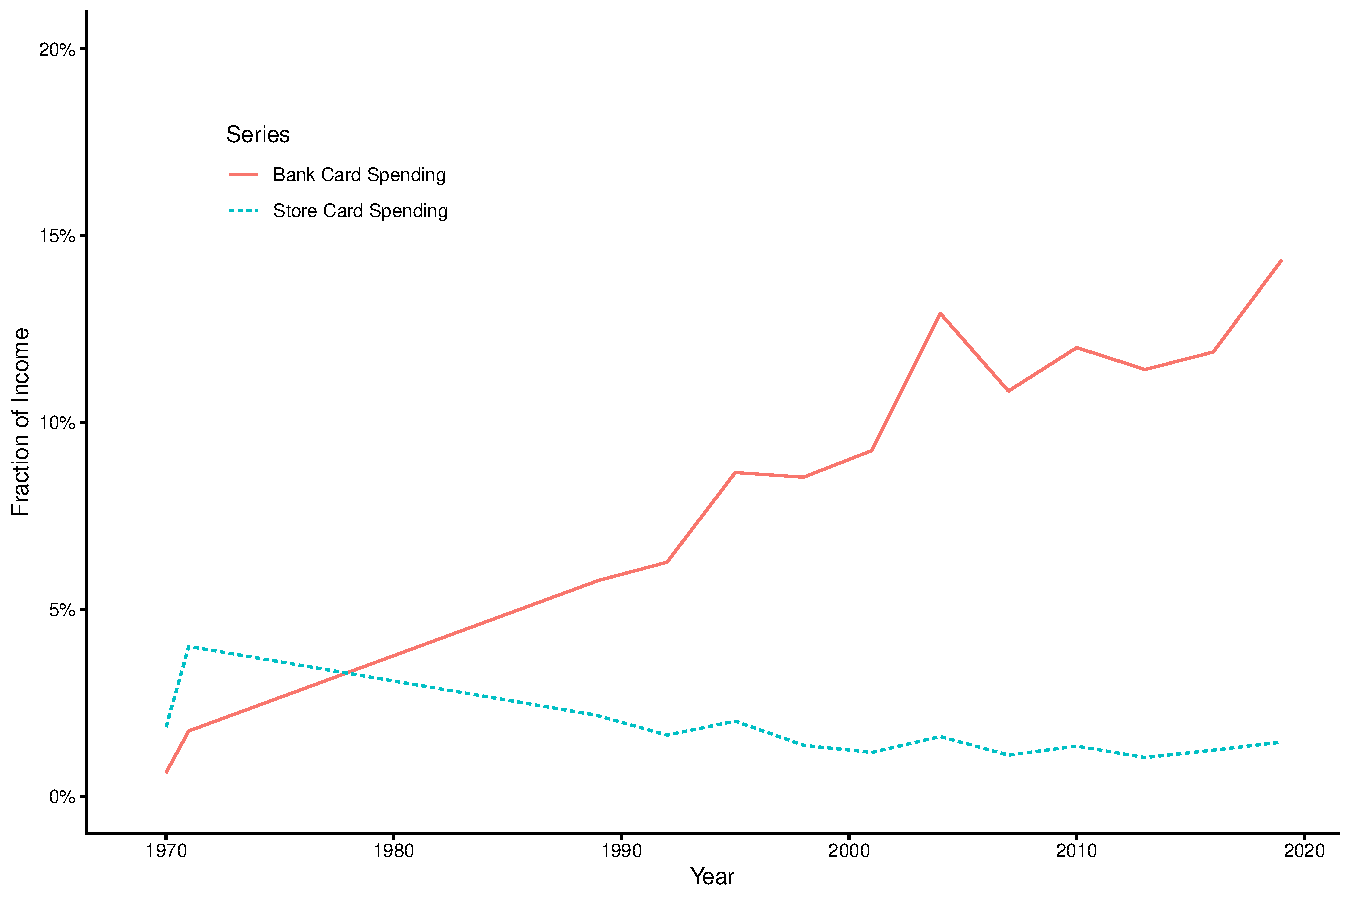
\includegraphics[width=\textwidth]{../Output/Figures/spending_levels.pdf}
     \end{subfigure}
     \hfill
     \begin{subfigure}[b]{0.45\textwidth}
         \centering
         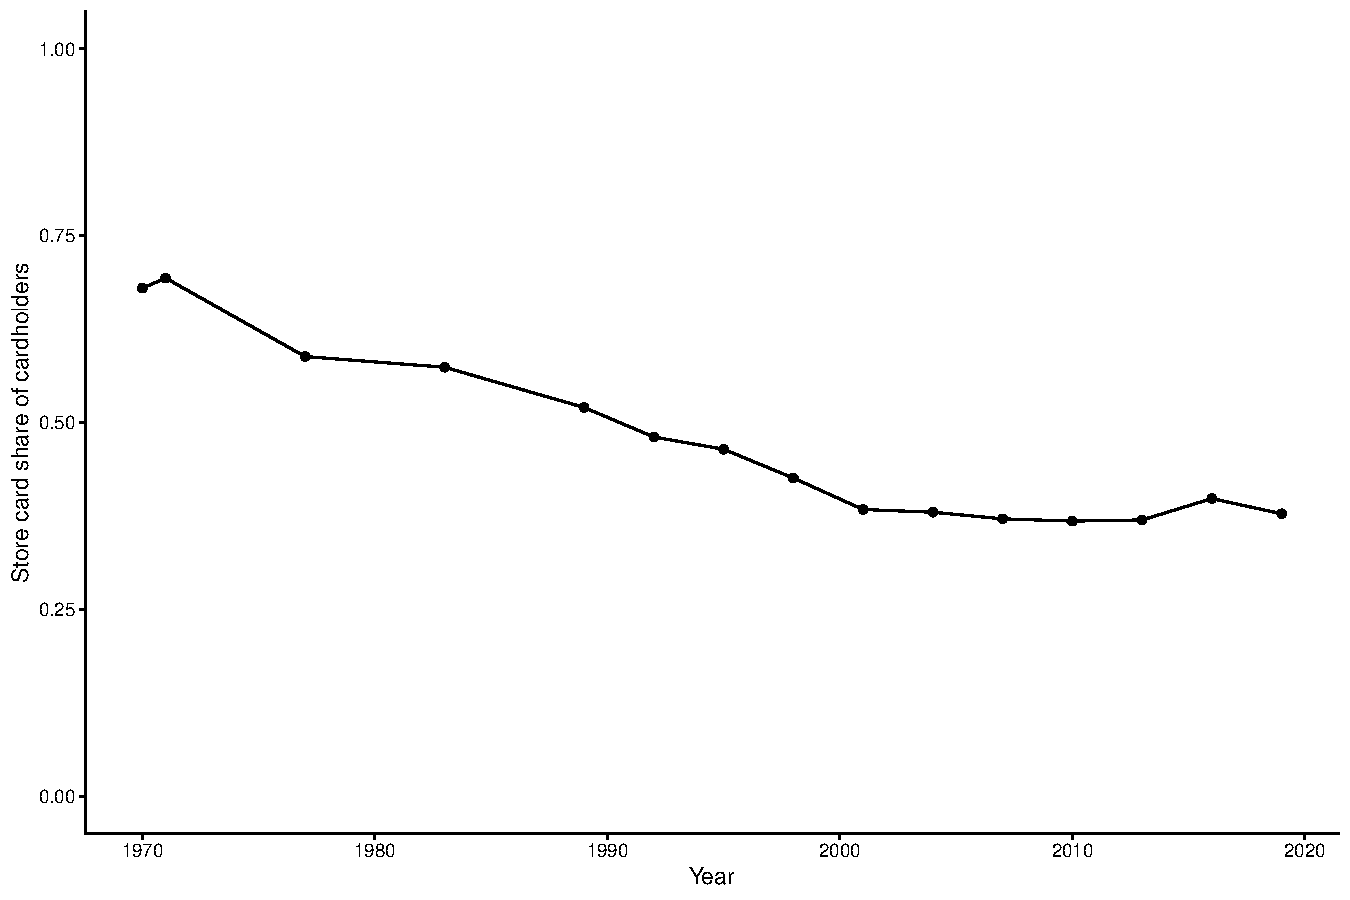
\includegraphics[width=\textwidth]{../Output/Figures/store_fraction.pdf}
     \end{subfigure}
     \newline 
          \end{center}
     \noindent \small \uline{Notes:} The figure shows the change in composition of credit card supply since 1970 (the first year in which the SCF inquired about credit cards) normalized by nominal income. ``Store Cards'' are cards that are only usable at specific stores, i.e. non-interoperable. Interoperable cards with store-specific branding are bank cards. Averages are weighted by SCF sample weights.
\end{figure}

Figure \ref{fig:bank_store} shows the changing composition of consumers' revolving credit over time. As can be seen the relative amount of credit card spending financed by stores (as opposed to banks\footnote{Following the SCF, I use "banks" to include all financial institutions, not necessarily those with ``banking licenses'' per se}), has been steadily declining since 1970. From 1970-1971, nearly 75\% of total credit card spending was on store credit cards -- as of 2019, that figure is less than 10\%. Bank credit cards proceeded to proliferate throughout the 1960s, and in 1970 the SCF added questions about credit cards to the survey for the first time, prefacing the question with ``There is a lot of talk about credit cards these days.'' Since the SCF tracks store credit borrowing in terms of balances, but credit cards in terms of spending amounts, I take the most conservative possible approach and only compare store credit card spending to bank credit card spending starting in 1970; the fraction of credit extended by stores early in the sample would be higher if I were to additionally attempt to estimate the flow of spending using store credit. 

The transition from store to bank consumer credit also shows up on the aggregate balance sheet of the retail sector. The Census publishes quarterly financial reports based on all firms nationwide with over \$50 million in assets, which has tracked receivables in a consistent way since 1980. Figure \ref{fig:receivables} shows the average quarterly ratio of outstanding receivables against quarterly revenue. In ``Retail Trade'', which are firms who sell directly to consumers, the fraction of receivables to revenue has fallen from 30\% to just over 10\% by the mid-2000s. To show that this is plausibly due to the proliferation of bank credit cards among consumers, and not a general intermediation of receivables in the economy, I plot the same series for the ``Wholesale Trade'' industry which operates with similar economics to retail trade, but sells to firms rather than directly to consumers -- this series is relatively flat at nearly 40\%.\footnote{Note that while the bulk of the decline in the time series of retail lending nationwide occurs from 1990 to 2005, this paper studies a cross-sectional change in retail lending occurring around 1977 to 1986 as described in Section \ref{sec:empirical-strategy} which I argue is causally identified. I therefore stress that the interpretation of the causal evidence is about a \emph{relative} decrease in store credit borrowing in states where bank credit cards expanded faster, at a time when, nationwide, store credit was still a large and growing industry.}

\begin{figure}[!ht]
 \caption{Receivables for Retail and Wholesale Firms}\label{fig:receivables}
 %\vspace{-0.25cm}
 \begin{center}
  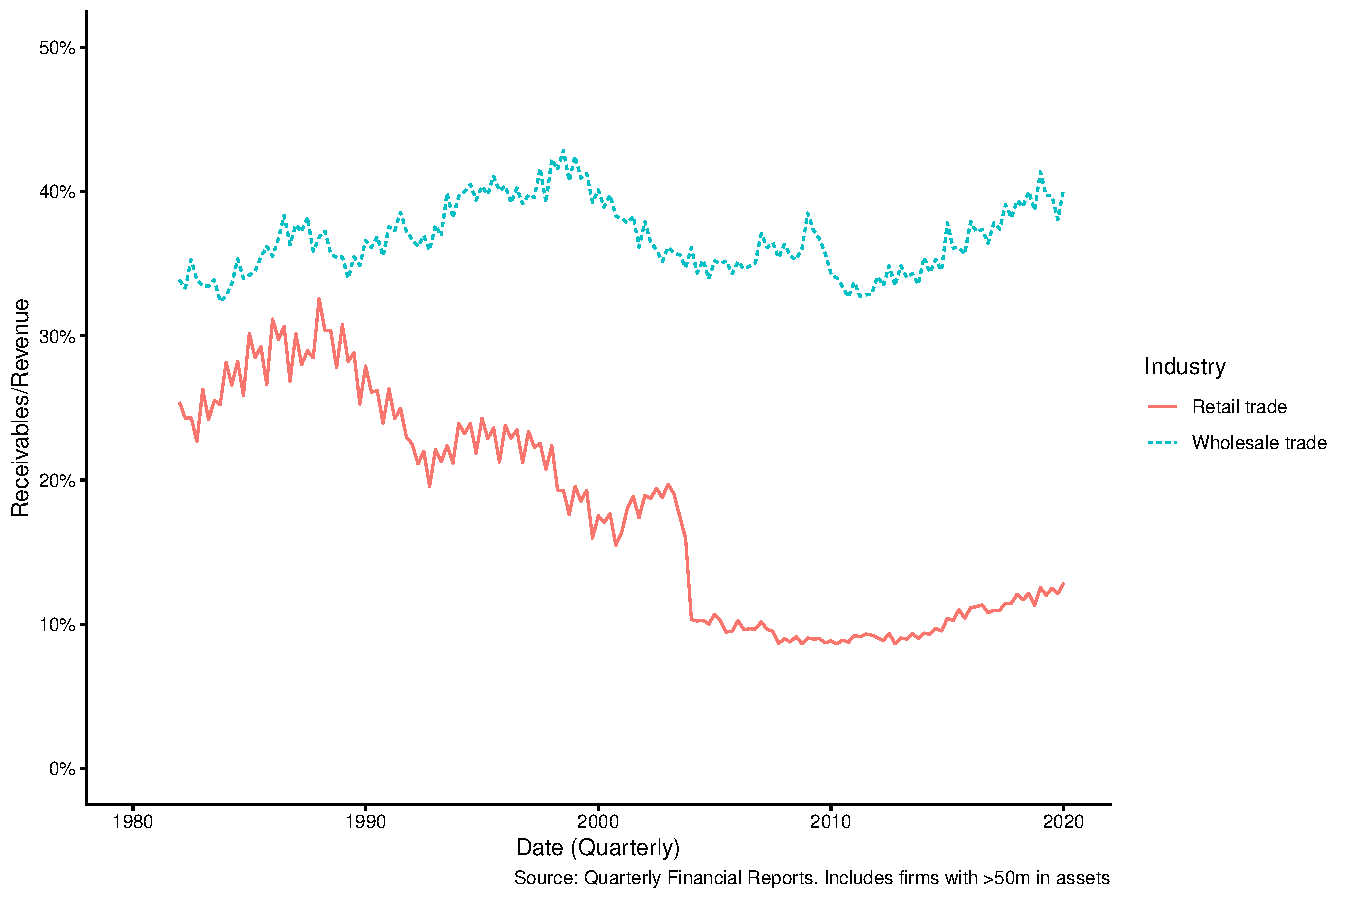
\includegraphics[width=.9\textwidth]{../Output/Figures/receivables.pdf}
  \end{center}
  %\noindent \small \uline{Notes:}  
\end{figure}

Historical sources also emphasize the importance of the high labor costs of store credit; the merchant interviewed in \cite{nocera_piece_2013} had three full-time employees dedicated to invoicing. The transition away from store credit does in fact show up in the aggregate wage bill of the retail sector -- Figure \ref{fig:backoffice_retail} uses census data broken down by wage and industry to show the dramatic decline of two occupations which supported the administration and collection of retail firms' receivables: bookkeepers and bill collectors. Retail firms once spent 4\% of their wage bill on workers in these two job roles which has declined by a factor of more than 10. While a decline has also been observed in the Wholesale industry of about 63\% since 1960, the decline over that same time period in the retail sector has been more pronounced at 78\%. 

\begin{figure}[!htp]
 \caption{}\label{fig:backoffice_retail}
 %\vspace{-0.25cm}
 \begin{center}
  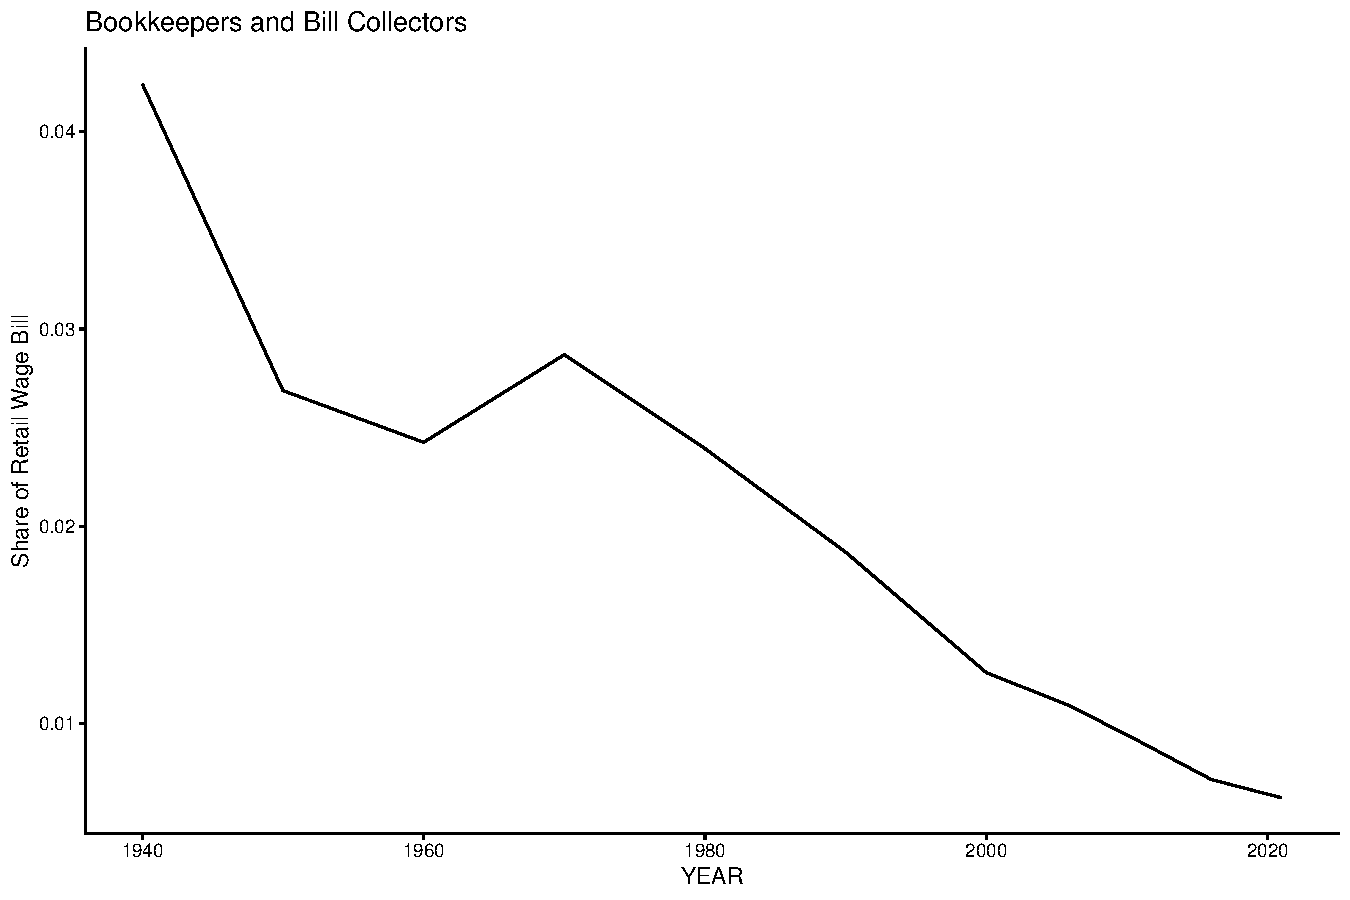
\includegraphics[width=.9\textwidth]{../Output/Figures/backoffice_retail.pdf}
  \end{center}
  \noindent \small \uline{Notes:} In each year, the denominator is the sum of wages of employees whose industry of employment (1950-standardized codes: IND1950 in IPUMS) is between 636 and 699 (retail trade). The numerator is the sum of wages of such employees whose occupation (1950-standardized codes: OCC1950 in IPUMS) is 320 or 321 (bookkeepers and bill collectors). \newline 
\end{figure}
%\vspace{-0.5cm}

I conclude this section by considering the international cross-section of countries by composition of consumer credit. This is important because other countries may wish to learn from the experience of the United States when considering the regulation of consumer finance in their own countries. Using the World Bank Findex (See Appendix \ref{sec:data} for details), I create Figure \ref{fig:international} which shows the distribution of countries by credit card ownership and store credit access with selected annotations. The United States is at the right tail of credit card usage with credit card ownership being more than 4x higher than store credit usage. Many prominent developing countries have much higher rates of store credit borrowing and almost all have much lower usage of credit cards. Therefore, while it may not be the case in the United States today that the cost and risk to businesses of issuing store credit to their customers is first-order, as bank credit cards have come to dominate in the equilibrium which exists in the United States today, the findings herein may be of importance for developing economies weighing the costs and benefits of expanding the consumer credit supply of banks. While Figure \ref{fig:international} does not show an unconditional negative correlation between store credit and bank credit card borrowing as one might expect, this is due to large cross-sectional differences across countries in overall financial development and consumer credit demand. No causal claims can be made from this exercise, but it is instructive to know that the levels of credit card ownership across countries vary from 0 to 80\%, and store credit usage from 0 to 45\%, and that countries exist at all four extremes (high/high, high/low, etc.). 

\begin{figure}[!htp]
 \caption{Credit Cards and Store Credit Internationally, 2011-2017}\label{fig:international}
 \vspace{-0.25cm}
 \begin{center}
  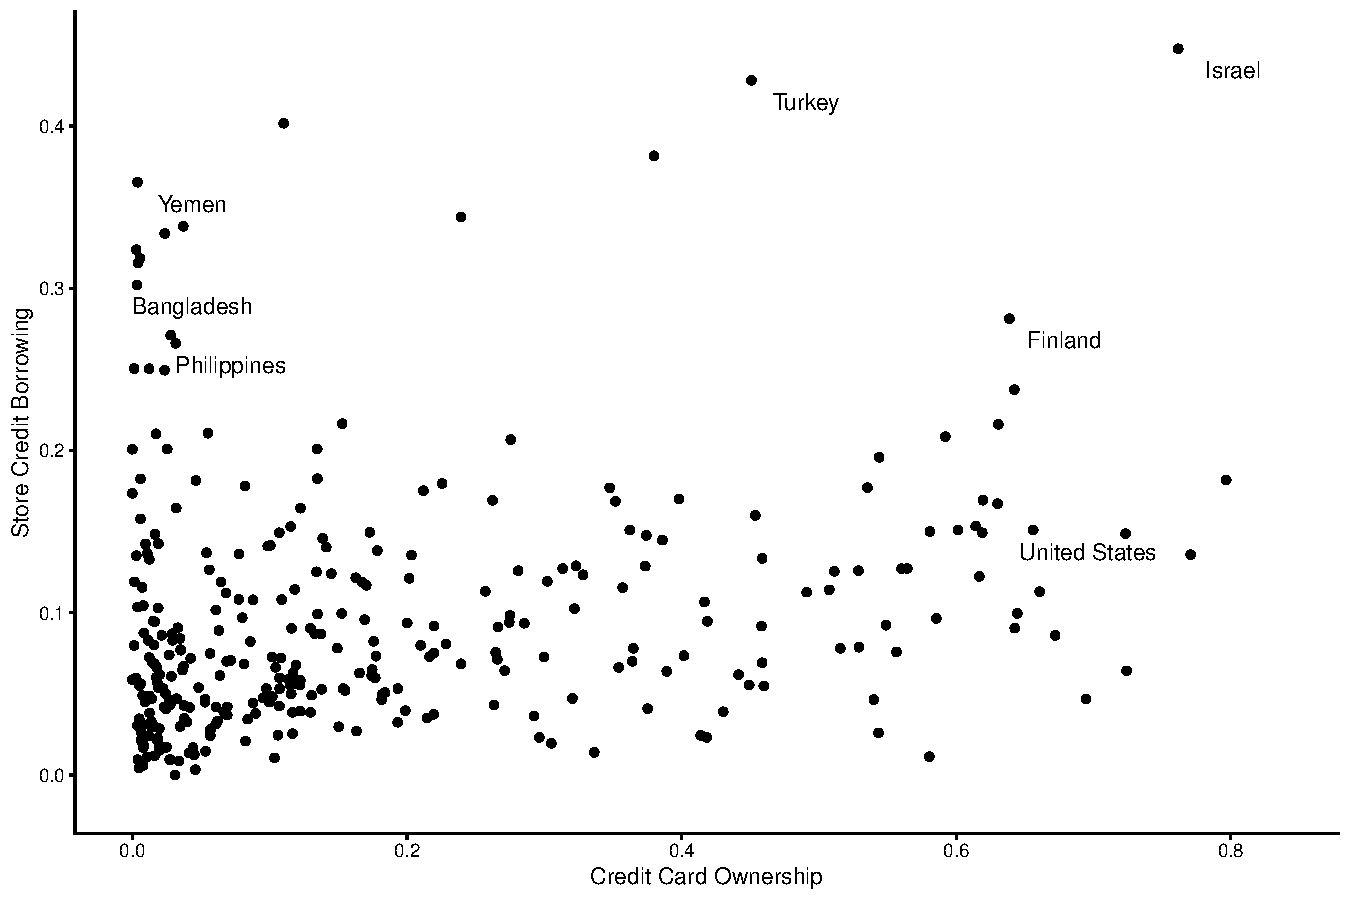
\includegraphics[width=.9\textwidth]{../Output/Figures/international.pdf}
  \end{center}
  \noindent \small \uline{Notes:} The figure shows the distribution of countries by (a) credit card ownership rates and (b) store credit usage rates, using the most recent available year for each country from the World Bank Global Findex (\cite{global_findex_2021}). The red dashed line marks the United States' position in each distribution.
\end{figure}

\section{Theoretical Framework}\label{sec:model}

In this section I give a decomposition based on accounting identities to pose the question precisely and sharpen the measurement exercise. In particular, I decompose the change in firm profits into a term due to changes in costs, and a term due to changes in markups. The main theoretical result is that any change in the aggregate profits of the retail industry can be decomposed into a change in markups and a change in costs, appropriately scaled. 

Estimating changes in marginal costs and markups separately is challenging, especially in the absence of per-unit price data. I therefore consider the problem in a very general way, without assumptions on the functional form of demand. The model only considers aggregate revenues ($P\times Q$) and aggregate costs ($C\times Q$), a highly attractive feature when working with data aggregated at the level of firms and industries, rather than product-level data with detailed product characteristics and prices with strong assumptions about the patterns of substitution between a large number of products at the scale of the entire retail sector. %Cite Matray, Klenow 

Instead of assuming a specific model of rebates and preferences across payment methods, (as in, e.g., \cite{rochet_platform_2003}, \cite{edelman_price_2015} and  \cite{wang_regulating_2023}) I assume that the introduction of new payment technology moves from one equilibrium denoted by $t$ to a new equilibrium denoted by $t+1$ where the levels of costs and competition (markups) are allowed to vary arbitrarily. Retailers' marginal cost, denoted $C_t$, is defined as the net cost of serving a customer inclusive of all direct costs of goods, labor costs associated with credit administration (screening, billing, collections), default losses from unpaid receivables, and any processing fees paid to payment networks (interchange or merchant discount fees). This ``all-in'' definition of cost is appropriate because it captures the full resource cost that a retailer must bear to complete a credit-financed transaction. $C_t$ is therefore net of all fees and risks, and and the outcome of strategic interactions and price-setting behavior between firms is summarised by the percentage markup $\mu_t \equiv \frac{P_t - C_t}{C_t}$. While the model in this section is general and does not assume any specific price-setting behavior of firms, I present a specialization of this model in Section \ref{sec:structural} which assumes that firms optimally choose $\mu$ in order to maximize profits, and that $\mu$ is a function of how differentiated firms are. Credit card networks may change this differentiation, e.g. by allowing customers to substitute between firms more easily if both accept a common payment method. $\mu_t$ should be thought of as a measure of how substitutable firms are -- if they are perfect substitutes, $\mu$ is close to 0. If they are differentiated, $\mu$ is greater than 0.

This fixes ideas and clearly defines the quantities that must be estimated in Section \ref{sec:profits}. While the evidence in Section \ref{sec:substitution} is clear that bank cards outcompeted store cards, it is not clear whether this transition benefitted or harmed firms in the retail industry. The two-sided market literature (see, e.g., \cite{rochet_platform_2003}, \cite{bourguignon_card_2014}, and \cite{wang_regulating_2023}) emphasizes that a credit card network need not benefit merchants (the less price-elastic side of the market) even when all merchants choose to join voluntarily, due to the negative externality imposed by one firm on another when it joins the network and steals business from its neighbor. The model presented herein will formalize this intuition in a very general way and suggest specific predictions which can be taken to the data to determine which of these two major effects, interoperability or cost-reduction, dominates. 

\subsection{Decomposition}

%Log-concave demand (Why do we need this again?) 
Let the marginal cost of a retailer be $C_t$. Define $\mu$ to be the markup above marginal cost such that $P_t = \left(1+\mu_t\right)C_t$. ``Financial technology'' may arbitrarily change $C_t$ and $\mu_t$, e.g. by interoperability of credit cards reducing consumer frictions to substituting between merchants. $Q(P)$ is an arbitrary demand function assumed to be constant over time. The following accounting identity holds, firm-by-firm and in the aggregate: 

\begin{comment}
This equation is false: 
    $$\underbrace{\frac{\left(P_{t+1}-C_{t+1}\right)Q_{t+1} - \left(P_{t}-C_{t}\right)Q_{t}}{P_t Q_t}}_{\Delta\mathrm{Profits}} = \underbrace{\left(\mu_{t+1} - \mu_t\right)}_{\Delta\mathrm{Markups}} \times \underbrace{\frac{P_{t+1} Q_{t+1} - P_t Q_t}{P_t Q_t}}_{\Delta\mathrm{Revenue}}$$ 
\end{comment}


\begin{equation}\label{eq:decomposition}
    \underbrace{\frac{\left(P_{t+1}-C_{t+1}\right)Q_{t+1} - \left(P_{t}-C_{t}\right)Q_{t}}{P_t Q_t}}_{\Delta\mathrm{Profit\,rate}} = \underbrace{\mu_{t+1}}_{\mathrm{New\,markup}} \times \underbrace{\frac{P_{t+1} Q_{t+1}}{P_t Q_t}}_{\Delta \mathrm{Revenue}} - \underbrace{\mu_t}_\mathrm{Old\,markup}   
\end{equation}

%Linearize this to show the condition that delta mu > mu delta R 

Let $\Delta\mu$, $\Delta C$, and $\Delta \mathrm{Revenue}$ represent the changes in $\mu$, $C$, and $PQ$ respectively; $\Delta\mu = \mu_{t+1} - \mu_t$, $\Delta C = \frac{C_{t+1}}{C_t} - 1$, and $\Delta \mathrm{Revenue} = \frac{P_{t+1}Q_{t+1}}{P_tQ_t} - 1$. Then linearizing Equation \ref{eq:decomposition} to a first-order approximation around $\Delta \mathrm{Revenue} = 0$ and $\Delta \mu = 0$ gives the following decomposition of profit changes into markup and revenue changes: 

\begin{equation}\label{eq:decomposition2}
    \Delta \mathrm{Profit\,rate} \approx \mu_{t} \Delta \mathrm{Revenue} + \Delta \mu  
\end{equation}

In order to decompose this further into explicit changes in cost, let the market equilibrium elasticity of demand be $\sigma$ such that $\frac{\partial Q}{ \partial P} \frac{P}{Q} = -\sigma < 0$. Crucially, I make no assumption about the relationship between the market-level elasticity of aggregate demand $\sigma$ and the price-setting behavior of any one firm which is summarized by the markup $\mu$. Then I can rewrite the change in revenue in terms of change in cost, obtaining:

\begin{equation}\label{eq:decomposition3}
    \Delta \mathrm{Profit\,rate} \approx - \left(\sigma-1\right) \mu_t  \Delta C + \Delta \mu 
\end{equation}

This holds firm-by-firm as well as in the aggregate. The main insight from this decomposition is that when a technology changes both markups and costs, the effect on profits is a horse race between the two. Holding markups fixed, the only other variable in the model that can exist to explain a profit increase is therefore a cost decrease. Crucially, this decomposition implies that the change in revenue can be interpreted separately from the change in markups without any product-level information on unit prices and quantities. This decomposition is useful because the changes in dollar profits, dollar revenues and dollar accounting costs can be measured without needing to take a stand on substitution patterns between an extremely large variety of goods on the scale of the entire retail sector. Therefore every term in this composition can be directly calculated from accounting data for firms where it is available. Dollar profits can also be proxied for by net entry (which is exactly true in, e.g., \cite{hopenhayn_entry_1992} and \cite{melitz_impact_2003}) when accounting data is not available, as I do in Section \ref{subsec:net_entry}. 

%This model does not nest platform fee models such as those cited only because retailers' costs are deadweight loss, whereas in network models they are frequently rebated to customers or networks. Indeed, this well describes the U.S. system of network interchange but not that of the U.K. and E.U., where interchange is regulated to much lower levels. Before 1986, however, credit card cash rewards for consumers did not exist (\cite{turner_credit_2012}), so this model well describes this setting. 

A limitation of this very general framework is that without any assumptions imposed on the demand function, it does not imply any particular quantitative mapping from a change in costs to a change in revenues. Backing out a quantitative estimate of costs requires further assumptions, an exercise which I perform in Section \ref{sec:structural}, estimating a cost reduction of 3.9\%.

%Furthermore, without explicitly modeling the entry and exit process, there is no quantitative mapping from an increase in profits to an increase in net entry. Therefore it is not possible in this framework to quantitatively map my estimate of a 4\% increase in net entry (my preferred sufficient statistic for economic profits) to a specific value of $\Delta \mathrm{Profits}$. It compares reasonably to, e.g.,  \cite{basker_raising_2012}, who finds that retail barcode scanners, a comparably significant retail technology innovation, increased labor productivity by 4.5\%. Another limitation is that without assuming any specific micro mechanism underlying consumers' and merchant's choices to join credit card networks and set prices, the model cannot make micro predictions about two-sided network fees in the spirit of \cite{rochet_platform_2003}. 

%What would CES demand imply here?

%This is like exactly equivalent to something Hsieh Klenow wrote, map it 

\section{Empirical Strategy}\label{sec:empirical-strategy}

%Describe how your data maps to the model 

\subsection{The Unexpected Deregulation of Usury Limits}

To estimate the effect of lending technology on store profits and store markups requires an instrument that satisfies an exclusion restriction, namely that it not affect store profits or markups by any channel other than via its effects on lending technology. I do this by examining a narrow regulatory shock which only affected the supply of consumer credit cards, not other forms of credit, was not anticipated, and was a shock to the cross section of entire markets, in this case states. As discussed in Section \ref{sec:trends}, the \emph{Marquette} decision by the US Supreme Court in 1978 provides such an ideal shock. 

 \cite{zinman_impact_2003} shows that previously-strict states saw a 4pp increase in credit card holding relative to previously-lax states between 1977 and 1983. Following \cite{zinman_impact_2003}, I define states as \say{treated} if the 1977 usury rate limit was less than 18\%, which was the most common prevailing usury rate limit at the time. ``Treated'' states are therefore Arkansas, Connecticut, Hawaii, Minnesota, New Jersey, Oregon, Pennsylvania, South Dakota, and Washington. I extend this work by showing the downstream consequences of credit card access on real economic variables in the resulting equilibrium.

It is important to clarify that my analysis uses the 1978 \emph{Marquette} Supreme Court decision as the exogenous shock, not subsequent state-level deregulation decisions. The usury rate in 1977 ($r_{77}$) defines treatment intensity, and the shock is the Supreme Court ruling that effectively made these limits non-binding for national banks operating across state lines. The subsequent voluntary removal of usury limits by state legislatures (e.g., 14 states by 1983) is an endogenous response to competitive pressure and is therefore not used as a source of identification. I choose not to exploit variation in other state-level regulations, such as restrictions on intra- or inter-state branching which were gradually removed by states generally throughout the 1980s. The objective of this paper is to narrowly identify the causal effect of consumer credit cards, separately from business lending and other forms of household lending such as mortgage and auto debt. Previous studies from  \cite{jayaratne_entry_1998} and \cite{mian_how_2020} have exploited the pattern of state-level deregulation of intra-state and inter-state branching restrictions to examine the macroeconomic effect of greater credit supply for households and businesses alike. I complement this literature by narrowly identifying the causal effects of one type of credit (household credit cards), rather than the macroeconomic effect of credit supply broadly. It is also important to note that state-level deregulation actions are frequently endogenous responses of legislators to industry pressure. 

\subsection{Relevance of Usury Limits}

The most common usury rate in 1977 was 18\%. The most direct evidence that this constraint was binding is that credit card interest rates in 1977 displayed extreme bunching at this limit, as shown by Figure \ref{fig:bunching}. Bunching is also observed at 12\% and 15\%, two other salient usury limits. By 1983, almost no bunching at the extremely strict 12\% and 15\% limits is observed whatsoever, and a significant mass of credit cards appear above the now-irrelevant 18\% cap. Bunching continues to be observed at 18\%, which \cite{knittel_price_2003} argue is due to collusion at this focal point, but is clearly no longer a binding cap, broadly. It is important to note that even if usury rates do not bind in equilibrium, their existence in the presence of uncertain inflation can still reduce credit supply.

\begin{figure}[!ht]
   \caption{Changes in bunching at usury rates}
        \label{fig:bunching}
     \begin{center}
         
     \begin{subfigure}[b]{0.45\textwidth}
         \centering
         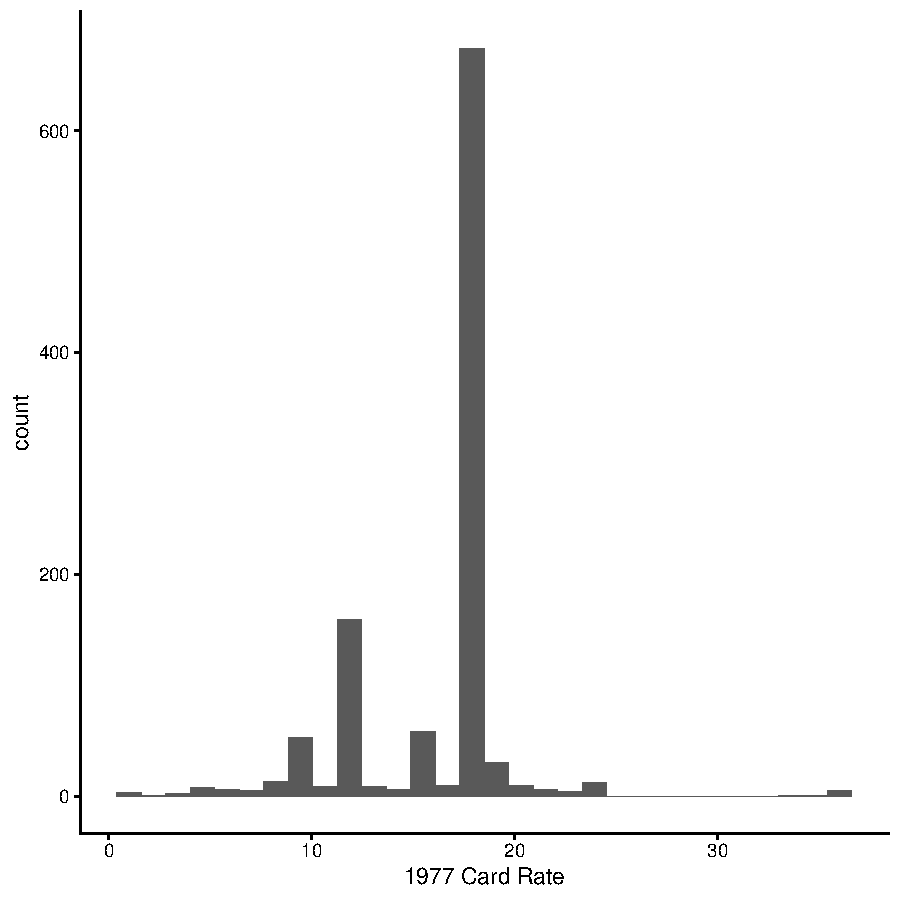
\includegraphics[width=\textwidth]{../Output/Figures/bunching.pdf}
     \end{subfigure}
     \hfill
     \begin{subfigure}[b]{0.45\textwidth}
         \centering
         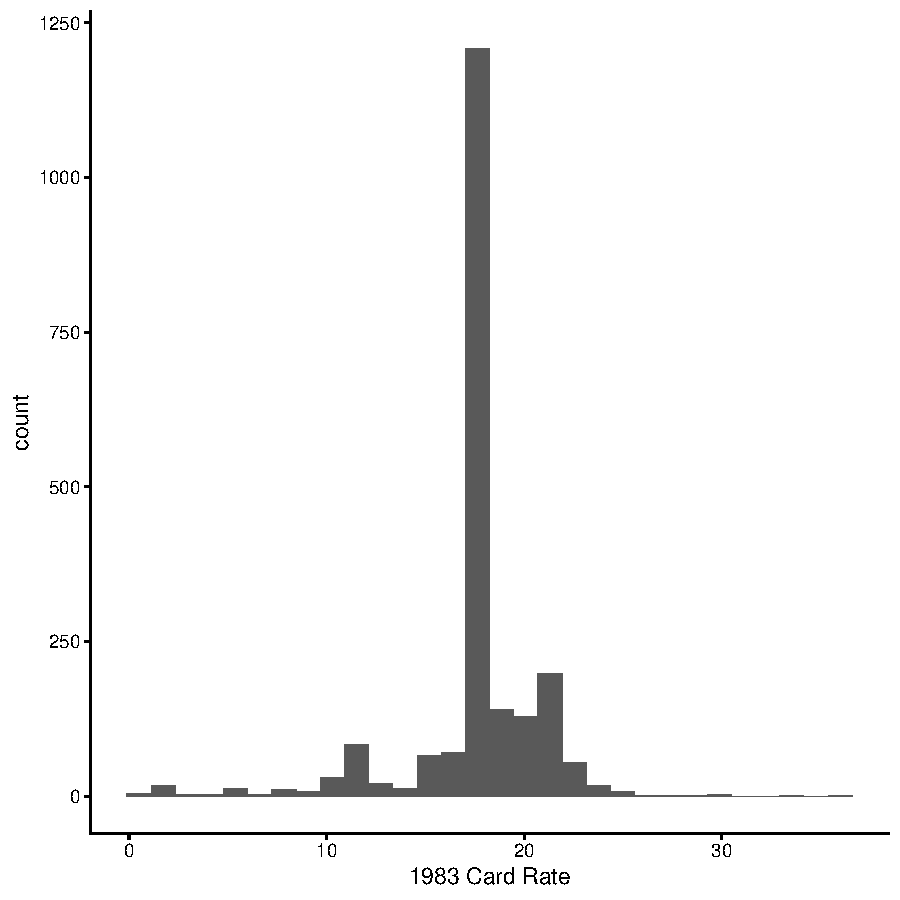
\includegraphics[width=\textwidth]{../Output/Figures/bunching_83.pdf}
     \end{subfigure}
     \newline 
          \end{center}
     \noindent \small \uline{Notes:} The figure shows the empirical distribution of bank credit card interest rates in the 1977 and 1983 Surveys of Consumer Finance. Since state-level identifiers are not available in 1977, only the nationwide distributions are shown. The most popular usury rates in 1977 were 12\%, 15\%, and 18\%. Usury rates were effectively abolished nationwide in 1978. 
\end{figure}

Usury regulation was especially potent due to the prevalence of inflation at the time. In the U.S. today, personal loan interest rate ceilings are often set at 36\%. In the  1970s and 80s, inflation and the federal funds rate reached as high as 17\%, higher than the usury rate in any of the states I consider \say{treated}. Figure \ref{fig:usury_ts} shows the time series of state average usury rates, compared to the rate of inflation and federal funds. I am therefore highly confident that the effect of \emph{Marquette} to deregulate these usury limits was material.

One might ask, then, why bank credit cards did not proliferate in the 1960s, when inflation was much lower. To a first order, the answer is that they did, but from a baseline of zero and facing significant inertia associated with the implementation of any new technology. Bank credit cards were indeed first introduced in the low-inflation environment of 1958-1959 in California and New York, and grew to the point of generating regulatory suspicion by 1969.\footnote{See ``Chase Bank Lists Credit Plan Gain'' (1959) and ``Law to Curb Unsought Credit Cards Foreseen'' (1969), Appendix \ref{sec:newspapers}} But their growth was hampered by the technological challenge of controlling fraud and authorizing large purchases in real-time. Indeed, it was not until 1971 that the first bank digital information system was able to connect bank branches to make lending decisions in real time.\footnote{Birmingham Trust National Bank: https://www.abandonedalabama.com/birmingham-trust-national-bank/} 

\begin{figure}[!ht]
 \caption{Usury Rates and Inflation, 1970-1990}\label{fig:usury_ts}
 \vspace{-0.25cm}
 \begin{center}
  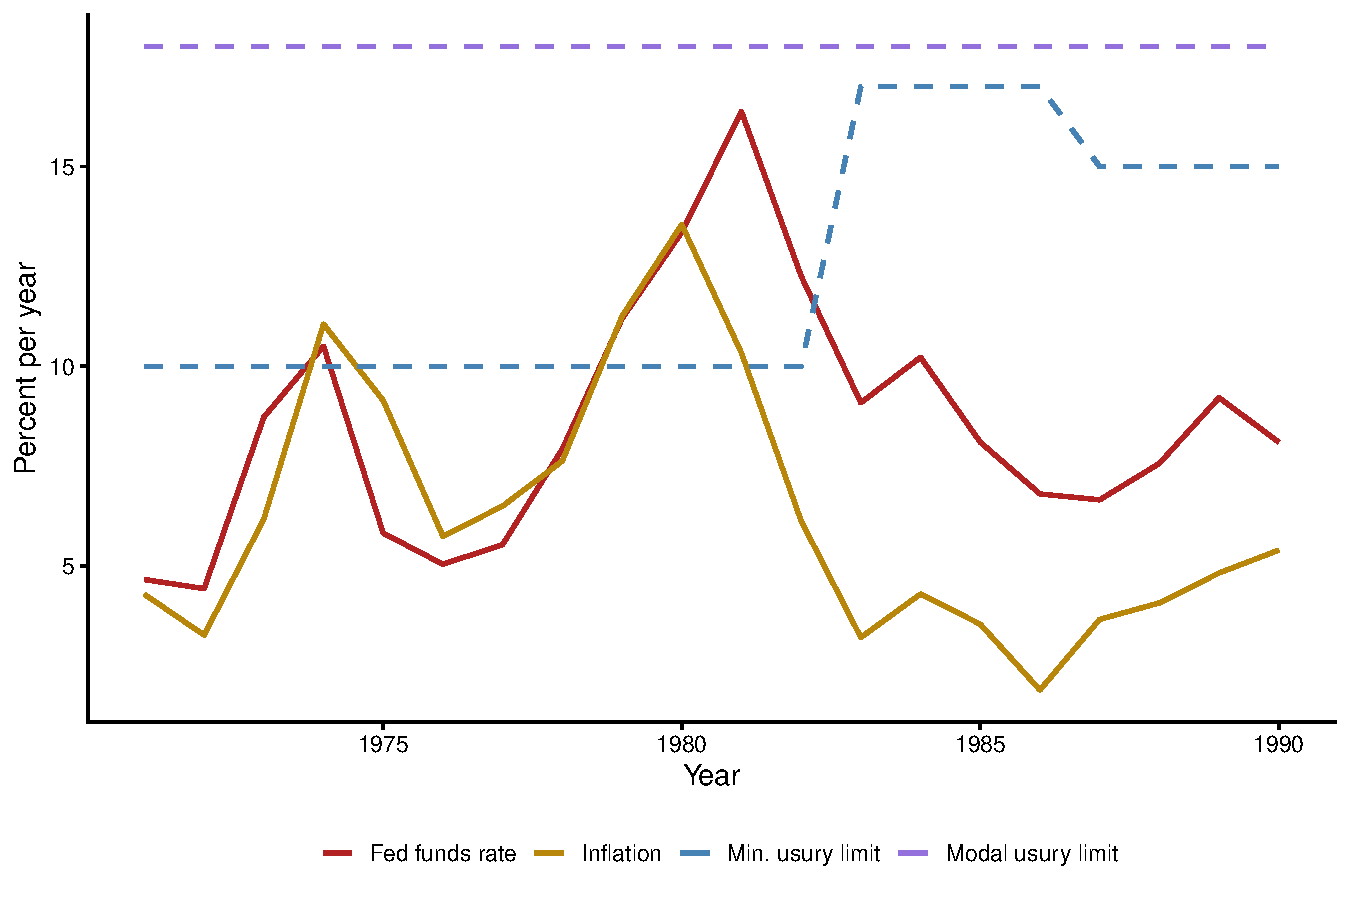
\includegraphics[width=.9\textwidth]{../Output/Figures/inflation_ts.pdf}
  \end{center}
  \noindent \small \uline{Notes:} The figure shows the timing of state-level usury deregulation in response to \emph{Marquette} in 1978, alongside the inflation and federal funds rates, a lower bound of banks' marginal cost of funds. 
\end{figure}

Figure \ref{fig:total_card_growth} shows the growth in total credit card lending in the United States scaled by nominal GDP, as well as the fraction of such lending originating in states without usury limits as of 1982. Credit card lending was barely \$50 billion in 1976, and grew to \$500 billion by 1990. Prior to 1982, less than 20\% of credit card lending originated in no-limit states -- by 1988 this fraction had grown to over 50\%. The growth of credit card lending also displays a notable kink after the deregulation of state-level usury limits, suggesting that usury deregulation played an important part in the rapid growth of credit card lending during the 1980s. In aggregate, the quantity of credit card lending scaled by nominal GDP more than tripled during this period, and almost all of the growth can be attributed to banks headquartered in deregulated states. 

\begin{figure}[!ht]
 \caption{Credit Card Growth}\label{fig:total_card_growth}
 \vspace{-0.25cm}
 \begin{center}
  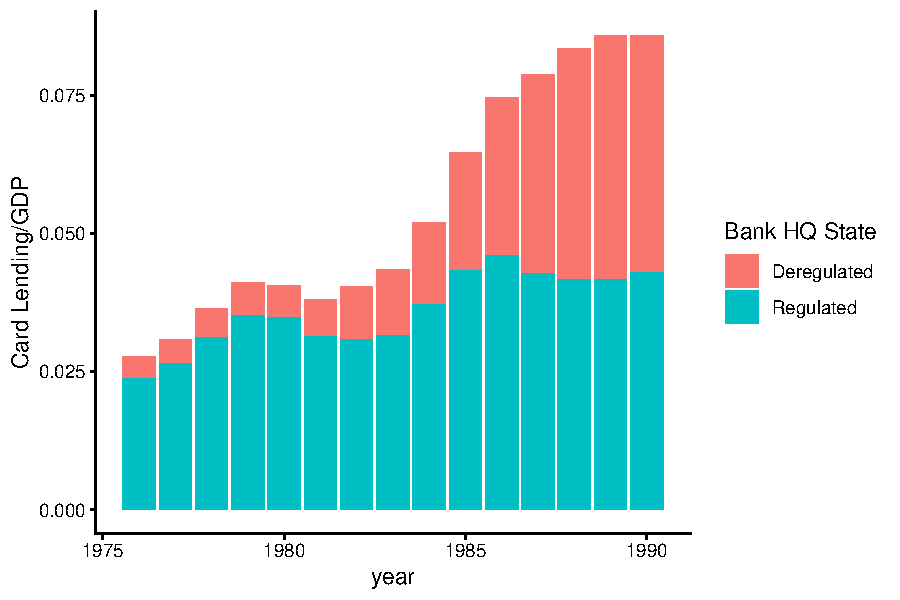
\includegraphics[width=.9\textwidth]{../Output/Figures/card_growth_stacked.pdf}
  \end{center}
  \noindent \small \uline{Notes:} The figure shows the aggregate growth in credit card lending by banks in the United States as recorded in the Call Reports. %The solid black line shows the aggregate credit card lending outstanding in billions of US Dollars (left axis). 
  Deregulated states are those who abolished usury limits by 1982: Arizona, Delaware, Illinois, Idaho, Montana, Nevada, New Hampshire, New Jersey, New Mexico, Oregon, South Dakota, Utah, and Wisconsin. Arizona removed its usury limit in 1981 and New Hampshire had no limit as of at least 1971; each other such state removed its usury limit in 1982. %Vertical lines mark 1978, the year of the \emph{Marquette} decision, and 1982, after several states deregulated to attract bank HQs. 
\end{figure}

Importantly, I do not argue that this particular evidence is itself informative about the causal effects of bank credit cards on retail firms. The reason is that Call Reports data is aggregated by the location of the lending bank, not the customer who borrows. These locations may not be the same, and indeed the content of the unexpected regulatory shock was to enable inter-state lending. Therefore I do not hypothesize that banks located in states with strict usury rates in 1977 would increase their credit card lending in response to \emph{Marquette}, but rather that banks located in high-limit or no-limit states would increase credit card lending across state borders to consumers in states in which tight usury limits still bind local banks. This particular evidence is important for establishing the relevance of the shock, but is not in itself useful for identifying its causal effect. This evidence is also useful to establish the time window in which the financial system re-optimized in response to \emph{Marquette}, justifying my decision to focus mainly on changes from 1977 to 1983. 

Another point which is crucial to the relevance of the instrument is that usury regulation disproportionately held back bank lending relative to store lending. This is because merchants have historically always been able to get around usury regulation by charging a different cash vs. credit price, as well as by using credit to drive sales even if lending itself is unprofitable. A bank which loses money on lending will not lend, whereas a merchant may choose to take losses on credit in order to sell a high-markup product. For this to be true it is critical that credit is a loss-leader for products in the store credit card market. To show this, I compare credit card interest rates by lender in Figure \ref{fig:card_rates}. I find that a large fraction---approximately 30\%---of store credit cards carry zero interest according to the SCF, compared to only 5\% of bank credit cards, suggesting that stores subsidize consumer credit, presumably in order to drive sales. This is not undone by differences in fees (which are similar between the two card types (\cite{consumer_financial_protection_bureau_credit_2022}), or compensation for greater bank card risk (store credit cards have \emph{higher} charge-off rates (\cite{consumer_financial_protection_bureau_consumer_2019}). The distributions of interest rates conditional on being positive are similar between the two types of lender. Existing studies of vertical integration between manufacturing, sales, and consumer finance have noted that captive lenders may charge higher or lower interest rates than standalone lenders. When external finance is scarce, captive lenders may offer cheap credit as a "competitive weapon" to increase their market share vis-a-vis smaller competitors (\cite{banner_competition_1958}). Indeed, General Motors has faced regulatory scrutiny for the anticompetitive effects caused by its ownership of General Motors Acceptance Corporation, which exclusively financed purchases of General Motors vehicles.\footnote{Emich Motors Corporation and U. S. Acceptance Corporation v. General Motors Corporation, 229 F.2d 714, 1956} Alternatively, captive finance lenders may offer higher rates as compensation for higher risk, if they find it optimal to target segments of the market where the parent manufacturer has larger market power (generally the low-credit-quality segment (\cite{benetton_credit_2022}). Captive finance companies may also have asymmetric information about credit quality and charge lower rates for that reason (\cite{stroebel_asymmetric_2016}). In the setting of U.S. credit card lending, the evidence from \cite{consumer_financial_protection_bureau_consumer_2019} that store cards have higher risk, and Figure \ref{fig:card_rates} that they charge lower rates, the competitive story is most consistent with the evidence: stores offer credit to consumers in order to close sales with customers who would choose not to purchase if only cash were accepted.

\subsection{Main Estimating Equations}

My key equations for identifying the causal effect of bank credit card access on economic outcomes are of the form: 

\begin{equation}\label{eq:dif_dif}
Y_{it}= \alpha_i + \gamma_t + \beta_{t\ne 1977} \cdot \mathbb{1} \left[ ru_{i,1977} < 18 \right] +  \varepsilon_{it}
\end{equation}

Where $Y_{it}$ are real outcome variables of interest, $\alpha_i$ are state fixed effects, $\gamma_t$ are year fixed effects, $\mathbb{1} \left[ ru_{i,1977} < 18 \right]$ is an indicator equal to one if the state had a usury limit lower than 18\% in 1977. $\varepsilon_{it}$ are error terms. $\beta_{t}$ are the outcomes of interest, which represent causal effects in year $t$, normalized to 0 in 1977. This design relies on the timing of the shock: as soon as the \emph{Marquette} decision was announced in 1978, the First National Bank of Omaha was immediately able to expand its credit card operations in neighboring Minnesota (a treated state), and others soon followed in other treated states. The sharpness of the timing of this deregulatory shock creates a natural placebo/falsification test of pre-trends, and allows me to naturally compare short-run and long-run effects. The fact that this estimation procedure produces a set of point estimates across time also creates a natural check of the reasonability of the estimates by whether they are relatively smooth over time, a further robustness check. 

In the firm-level analysis conducted in Section \ref{sec:substitution}, many firms have sales across multiple treated and untreated states. For such firms, I calculate the ``Treated'' variable as the sales-weighted average ``Treatment'' across sales locations. I also include firm fixed effects. 

To more narrowly test the hypothesis that any changes are due to bank credit cards displacing store credit cards, I focus on the clothing retail industry. As shown in Table \ref{tab:card_uses}, clothing was the predominant use of credit cards in the 1970s. I estimate the following triple-differences specification, where $j$ further disaggregates the data by sub-industry, focusing on $\beta_1,t$ as the series of outcomes of interest:

\begin{equation}\label{eq:triple_dif}
Y_{ijt}= \alpha_{ij} + \gamma_t + \beta_{1,t\ne 1977} \cdot \mathbb{1} \left[ ru_{i,1977} < 18, SIC2_j \in 56xx \right] + \beta_{0,t\ne 1977} \cdot \mathbb{1} \left[ ru_{i,1977} < 18 \right] +  \varepsilon_{ijt}
\end{equation}

This specification, by design, differences out any general equilibrium effects on either the supply side and demand side. Typically, financial economists believe that access to credit relieves entrepreneurial financial constraints and enables business formation. The assumption that I make in order to identify the effect of credit cards as instruments for transactions, separately from relieving entrepreneurs' budget constraints and changing customers' demand, is that these macroeconomic effects are not systematically different across sub-industries of retail in the same way that industries differ in usage of credit cards -- in particular, that the clothing retail industry relied on credit cards at this time uniquely more than other retail sub-industries. This empirical test is therefore more appropriate for testing whether the effect of credit cards depends on whether they are used to transact business, separate from whether they relieve credit constraints: a relief of budget constraints would induce higher consumption on all categories of goods, even on goods where the credit card is not used to transact business, because the overall budget constraint is relaxed. This triple difference is therefore preferable for evaluating the causal effect of interest when sufficient data is available, as it is in the case of net entry. 

\subsection{Validity of Parallel Trends Assumption}\label{subsec:validity}

I assume that all relevant outcome variables would have evolved in treated and untreated states in parallel in the absence of the 1978 \emph{Marquette} decision. This subsection provides evidences and arguments supporting this assumption. 

Firstly, there was no clear geographic pattern to usury regulation in 1977. Figure \ref{fig:rate_77} shows the usury rate in each state as of 1977. High- and low-usury limit states are roughly equally prevalent in coastal and inland regions, northern and southern regions, and eastern and western regions. 

\begin{figure}[H]
 \caption{State Usury Rates, 1977}\label{fig:rate_77}
 \vspace{-0.25cm}
 \begin{center}
  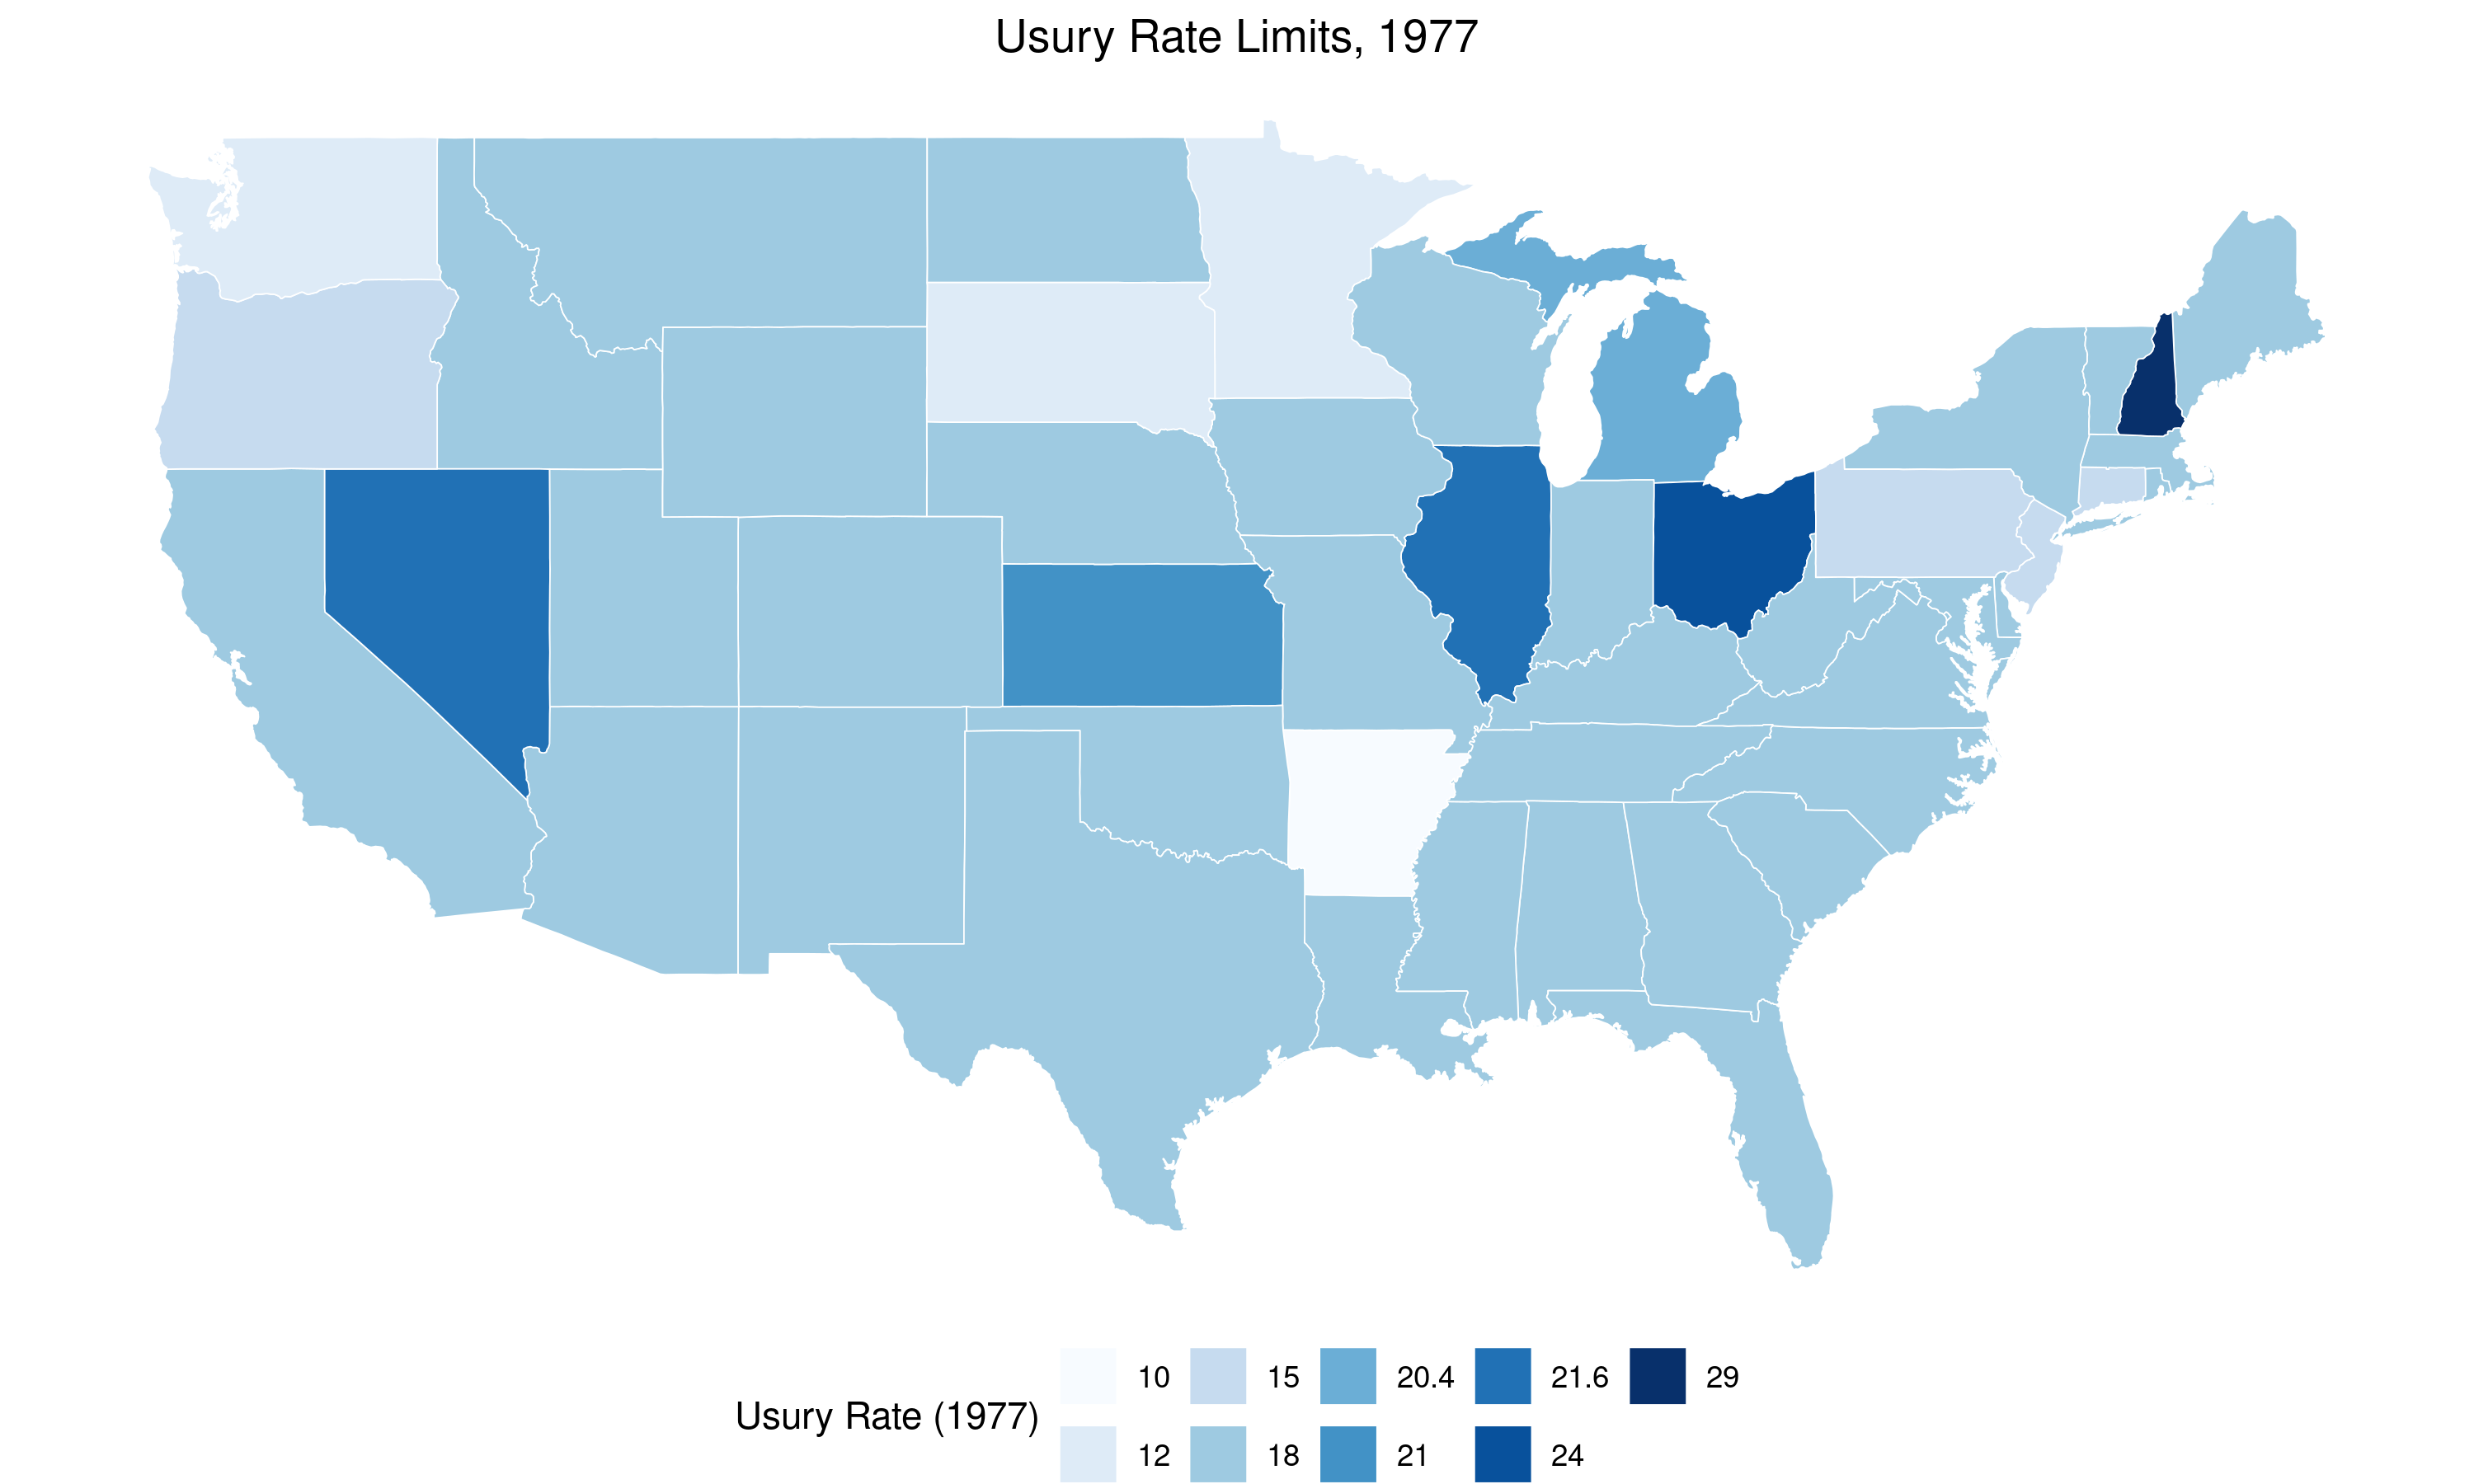
\includegraphics[width=.9\textwidth]{../Output/Figures/rate_77.png}
  \end{center}
  \noindent \small \uline{Notes:} The figure shows the usury rate (maximum legal interest rate) for consumer lending in each state as of 1977. \newline 
\end{figure}
\vspace{-0.5cm}

Secondly, the state of usury regulations in 1977 was uncorrelated with other measures of subsequent financial deregulation. \cite{mian_how_2020} calculate an aggregate index of deregulation from 1970-1990 and show that it predicts increases in credit growth generally. The correlation between my binary measure of treatment and the Mian-Sufi-Verner index of deregulation is -0.04, suggesting that any effect due to the effective interest rate deregulation of \emph{Marquette} was orthogonal to any subsequent deregulation decisions on the part of state legislatures. There is also no clear relationship between states which are \say{treated} from the perspective of household credit card access and states which chose to deregulate their own banks in 1982-1983: only New Jersey, Oregon, and South Dakota had both restrictive usury laws ex-ante in 1977 and also removed their usury limits in 1982-1983. 

Another concern one might have is that the Volcker disinflation of the early 1980s might have caused an increase in credit supply in states with lower usury rates, independent of \emph{Marquette} -- since usury rates are nominal, lower inflation would disproportionately affect states with low nominal rates. However, given the fact that states in which credit cardholding increases are orthogonal to states in which credit card issuance increases, I conclude that growth in inter-state lending is primarily responsible for this growth. If the cause were disinflation, I would expect to see banks in low-limit states expanding credit within that state; rather I see an increase in cardholding in affected states financed by  banks in other states, exporting their usury limits to affected states as became allowable by \emph{Marquette}. 

Furthermore, the historical origins of state usury limits suggest strong path dependence. Many usury limits trace their origins to colonial-era legislation, religious traditions prohibiting excessive interest, and 19th-century populist politics (\cite{glaeser_neither_1998}). These limits were typically set decades before the period of study and were not responsive to economic conditions in the 1970s. For example, Arkansas' strict 10\% constitutional usury cap dates to its 1874 constitution, while New Hampshire's absence of any cap reflects longstanding libertarian governance traditions. The persistence of these regulations across decades of economic change supports the interpretation that the 1977 cross-section of usury rates reflects historical path dependence rather than contemporaneous economic conditions, strengthening the plausibility of the parallel trends assumption. Table \ref{tab:treatment_balance} in the Appendix confirms that treated and control states are balanced on key economic characteristics as of 1977.

Finally, in my main difference-in-difference analyses I report the estimated coefficients on the treatment prior to the treatment time, which can be visually inspected for obvious violations of parallel trends. I extend the pre-treatment window back to 1970 where data are available, which encompasses the 1973-1975 recession and provides a more demanding test of the parallel trends assumption.

\section{Effect on Store Credit Supply}\label{sec:substitution}

To estimate the magnitude of the reduction in firm lending, I perform a difference-in-difference analysis using Compustat firms linked to sales locations in Dun \& Bradstreet. Firm and year fixed effects are included, so this analysis estimates the relative change in credit extended to customers based on where the firm's sales occur. 

\begin{figure}[H]
 \caption{Difference-in-Difference of Lending by Stores}\label{fig:dif-receivables}
 \vspace{-0.25cm}
 \begin{center}
  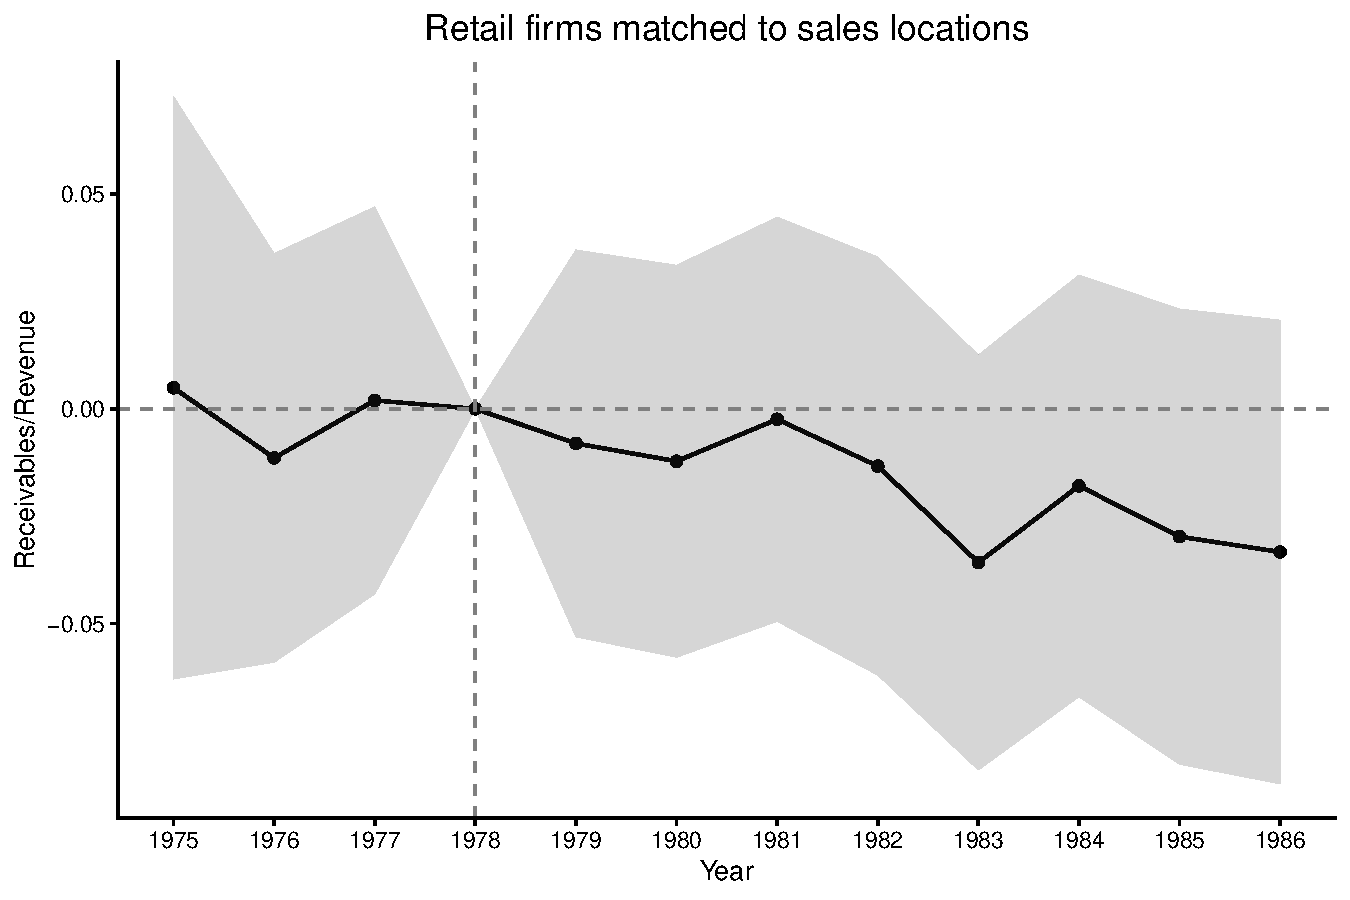
\includegraphics[width=.9\textwidth]{../Output/Figures/receivables_revenue.pdf}
  \end{center}
  \noindent \small \uline{Notes:} Sample of 179 retail firms based on accounting data from Compustat linked to sales locations in Dun \& Bradstreet, excluding firms with receivables-to-revenue ratios above 0.8. 95\% confidence intervals are shown in shaded bands. The year of \emph{Marquette}, when bank credit card lending increased more in ``Treated'' states, is denoted with a dashed vertical line. Default standard errors are shown, and robustness to state-level correlation is analyzed in Appendix \ref{sec:permutation}.
\end{figure}
\vspace{-0.5cm}

As can be seen, after the treatment there is a significant decrease in the amount of credit extended by stores to their customers from a base rate of 20\% by about 4\% by 1983. This is, if anything, likely to \emph{understate} the effect, because as the historical accounts discussed in Section \ref{sec:data} emphasize, smaller firms were more likely to benefit from accepting bank cards, and thus engage in this substitution, than were large firms. The bulk of the change is also observed after 1981 -- the average coefficient in the first 3 years after the treatment date is 68 basis points, whereas the average coefficient from 1982 through 1983 is 3.2\%. This is consistent with the fact that bank credit card lending accelerated most after 1981, as shown by Figure \ref{fig:total_card_growth}, when large banks including Bank of America and Citibank relocated their headquarters to no-limit states.

To estimate the crowd-out that bank credit imposes on store credit, I compare the estimates of the increase in bank credit to the decrease in store credit. As shown in Figure \ref{fig:bank_store}, the levels of spending in 1977 on bank and store cards were almost 1-to-1, meaning that comparisons of their percentages are equivalent to comparisons of their dollar values. The firm-side 1977 to 1983 estimate of a 4.4\% (Figure \ref{fig:dif-receivables}) decrease in store credit is directly comparable to the consumer-side 1977 to 1983 estimate of a 5.5\% (Table \ref{tab:zinman}), yielding a crowd-out estimate of 4.4/5.5 = 80\%.

I rely on estimates produced by \cite{zinman_impact_2003}\footnote{These estimates rely on nonpublic SCF state-of-residence data.} to calculate the increase in bank credit card supply from the consumer side, and complement them with original estimates from the firm side to estimate the extent to which bank credit crowded out store credit. 

%Selected Estimates from Zinman (2003) here 
\begin{table}[!ht]
\caption{Growth in Bank Credit Card Access}\label{tab:zinman}

\begin{center}
    \begin{tabular}{lccc}
   %\tabularnewline 
   \midrule 
   Dependent Variable: & Bank Card Rate & Has Bank Card & Has Any Credit Card\\  
%   Model:              & (1)\\  
   \midrule
  \emph{Variables}\\
   Treat x Post            & 1.39$^{***}$ &0.055$^{**}$ &0.011\\   
                       & (0.37) & (0.025) & (0.021)\\   
   \midrule
   \emph{Fixed-effects}\\
   State            & Yes  & Yes & Yes\\  
    Year            & Yes & Yes & Yes\\ 
   \midrule
   %\emph{Fit statistics}\\
   Observations        & 1,936 & 6,059 & 6,059\\  
   \midrule 
   \multicolumn{2}{l}{\emph{Standard errors in parentheses}}\\
   \multicolumn{2}{l}{\emph{Signif. Codes: ***: 0.01, **: 0.05, *: 0.1}}\\
\end{tabular}
\end{center}

\noindent \small \uline{Notes:} Selected estimates from \cite{zinman_impact_2003}. The estimates compare households by state in the 1977 vs. 1983 SCF. ``Treated'' states are those with usury limits below 18\% in 1977. 
\end{table}

As can be seen, bank credit card access increased substantially by 5.5 percentage points in the more-affected states from a mean of 38\%, an increase of 14\%. Bank card interest rates also increased significantly by 1.4 percentage points from a mean of 16.4\%, which is consistent with a binding price cap relieving a supply-side constraint. Interestingly, the fraction of consumers with access to any credit card, store or bank, stayed constant. This is consistent with bank cards substituting for store cards among consumers who had previously used store cards. 

%A potential concern is that errors are correlated between firms selling in the same state (e.g. demand shocks at the state-level). Because firms sell in multiple states, this is not easily overcome by clustering errors at the state-of-sales level as \cite{abadie_when_2017} would typically prescribe because the outcome variable (receivables/revenue) exists at the firm level. I address by using permutation testing at the state-of-sales level in the spirit of \cite{rosenbaum_design_2010} using the procedure described in Appendix \ref{sec:permutation}. 

\section{Effect on Firm Profits}\label{sec:profits}

A key takeaway from the model is that the effect of interoperable credit card systems on merchant profits is \emph{ex-ante} uncertain. I therefore estimate the effects of store-to-bank credit substitution using two measures of profitability: accounting profits and net entry. I measure accounting profits by calculating net income margins in firms for which these data are available (the Compustat sample), and measure net entry of firms using County Business Patterns. I also consider heterogeneous effects by industry according to the importance of credit card payments across industries. Both analyses confirm the result that the entry of bank cards, and reduction in store lending, are associated with higher profitability of retail firms. 

Each analysis has its strengths and weaknesses. Accounting data has the advantage of being interpretable directly in units of profit margins, tightly connecting the magnitude of estimates in this analysis to the model. The availability of data on receivables for these firms, and the analysis in Section \ref{sec:substitution}, also facilitates a natural comparison of the magnitude of the profitability change against the magnitude of the change in lending. Unfortunately, since accounting data is only available for 195 large retail firms in 1978, the power of the analysis of accounting profits has low power. Firm profits are extremely noisy, and driven by many factors much more important than credit card receivables and merchant discount fees. If administrative costs and credit chargeoffs were 10\% of receivables, and the fees charged to merchants by bank credit card networks were zero, I would expect the effect on the firm's aggregate profit margins to only be 36 basis points. Furthermore, there are many issues with interpreting accounting profits as economic profits, the most salient of which are (1) the inability to track marginal costs separately from total costs, (2) the importance of intangible assets and expectations of future profits. 

In order to overcome the difficulties in interpreting accounting profits as economic profits, I turn to another dataset which has much higher power, but where profits and receivables are not directly observable: the County Business Patterns, which is collected by the US Census Bureau and includes all formal establishments in the United States since 1947 (\cite{eckert_early_2022}). I rely on changes in net entry of firms as a sufficient statistic for increases in net profitability of pre-existing firms, as is the case in \cite{hopenhayn_entry_1992} and all models which inherit its structure such as \cite{melitz_impact_2003}. The CBP dataset is suited for this purpose as it includes counts of firms by narrow 4-digit SIC industry codes-cross-employment category. While this analysis is unable to speak to the quantitative relationship between net entry and profitability, it is more suited to making statistically powerful statements about whether the effect on net entry, which must have the same sign as the effect on profits, is negative or positive. This analysis has the added advantage of being able to control for any changes to entrepreneurial credit (supply-side) constraints by comparing the clothing retail industry, where cards are most used, to other retail industries which face the same supply-side shocks. These substantial advantages lead me to interpret this analysis as the most powerful and relevant test of whether bank credit cards made the retailer industry better off in general. 

In another analysis, I compare the attributes of firms which do and do not adopt bank credit cards, according to my novel Yellow pages data. The cost-reduction mechanism predicts that firms' incentive to adopt bank cards should increase when privately supplying credit is more expensive. Historically, large and geographically-diversified retailers like J.C. Penney were among the last to accept bank credit cards (\cite{hyman_borrow_2012}). I bring this prediction to my newly-collected data on merchant acceptance from the Yellow Pages and show that within narrowly-defined industry-by-city categories, firms with low geographic diversification were more likely to be early adopters of bank cards. Conversely, the competition mechanism predicts that the firms with the most incentive to adopt cards are those where competition between retailers is the tightest. I proxy for the competition between retailers by sales levels on the assumption that retailers with smaller market shares face tighter competition, an assumption which is true in most discrete-choice models of demand. Contrary to the predictions of this mechanism, I find that merchants with higher sales, and therefore less elastic demand, are more likely to adopt bank cards, ceteris paribus. 

I also compare the survival rates and sales growth of bank-card-adopting and non-adopting firms in treated and untreated states following the \emph{Marquette} shock. In contrast to the demand-steering story, I find that the relative sales of accepting firms in treated states \emph{decreased}. However, their length of survival increased. This is another piece of evidence inconsistent with demand-steering and consistent with cost-reduction. 

%The mechanism of intensified competition also makes direct predictions about the cross-elasticity of sales between firms, namely, that increases in bank card usage will increase that elasticity. I can test this by looking directly at whether bank credit cards intensify competition between retail firms. I approach this using a novel design based on the responses of sales of existing firms to new entrants and apply my difference-in-difference design to state-by-year estimates of these elasticities. 

Finally, I consider evidence for two specific channels by which bank cards may reduce cost, which are labor cost reductions and the ability for bank cards to effectively insure firms against credit risk in their customer base. I find that bookkeepers' and bill collectors' share of retail firms' aggregate wage bill decreased from 4\% to less than half a percent from 1940 to 2020, and that treated states had a 3\% higher relative rate of survival in the 1983 recession than firms in untreated states. 

\subsection{Net Entry}\label{subsec:net_entry}

To overcome the limitations of accounting data, namely (1) the discrepancy between accounting profits and economic profits and (2) the small universe of retail firms with 1970s-era accounting data available, I analyze net entry of firms as my preferred sufficient statistic for economic profits. This allows me to extend my sample to retail firms of all sizes which are accounted for in the Census County Business Patterns, and to do heterogeneity within narrowly-defined industries. Following the evidence in Table \ref{tab:card_uses}, I compare the clothing retail industry to all other industries using the triple-difference specification of Equation \ref{eq:triple_dif}. 

%Reiterate why this is a good test 

\begin{figure}[H]
 \caption{Triple-Difference Analysis of Establishment Counts by Size: Clothing Retail Industry}\label{fig:clothing_dif}
     
    \begin{center}

     \begin{subfigure}[b]{0.3\textwidth}
         \centering
         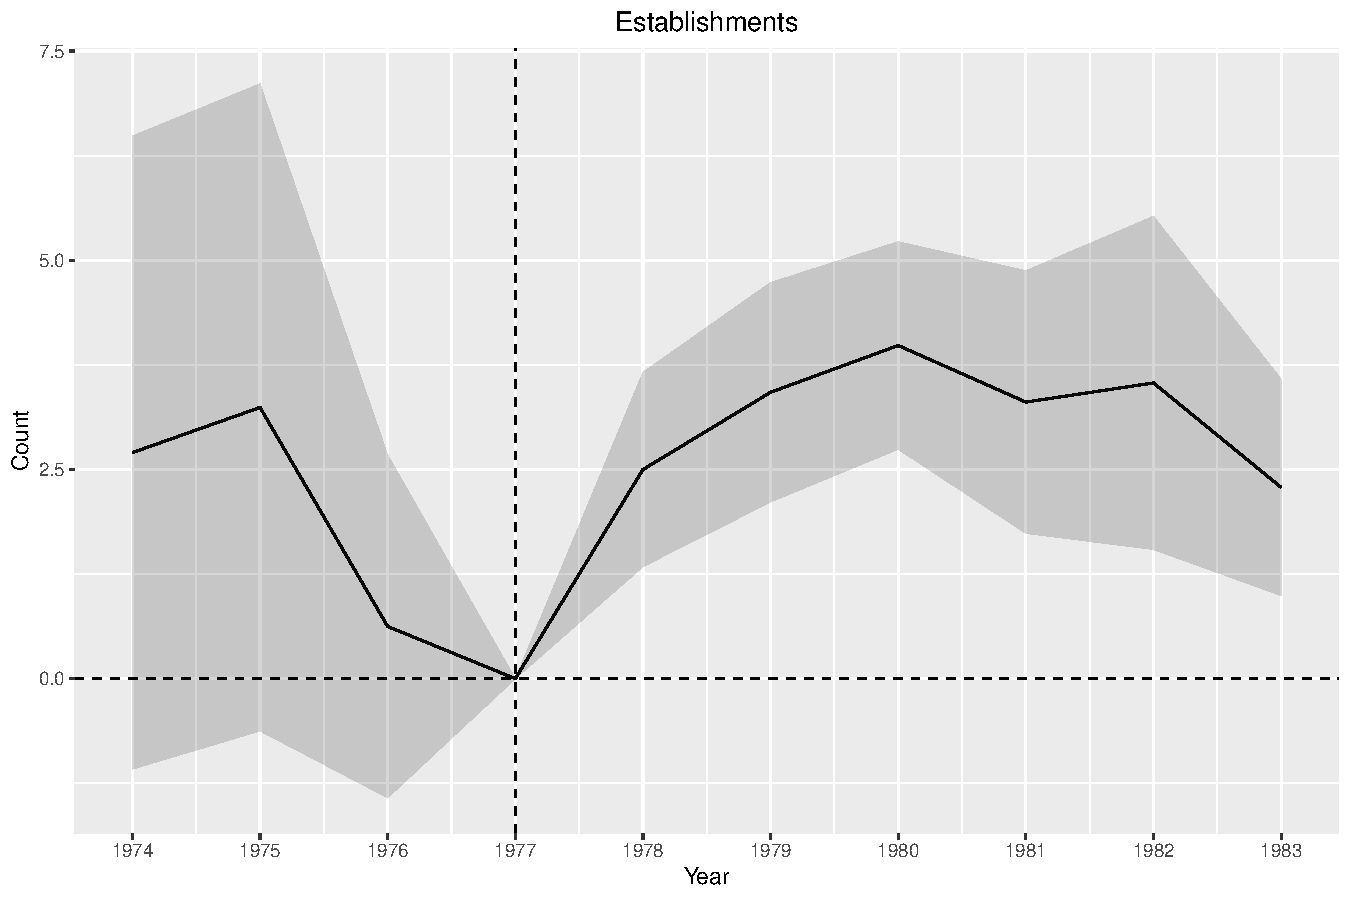
\includegraphics[width=\textwidth]{../Output/Figures/est.pdf}
         \caption{Establishments}
    \end{subfigure}
         %\hfill
         \hspace{0.65cm}
         \begin{subfigure}[b]{0.3\textwidth}
         \centering
         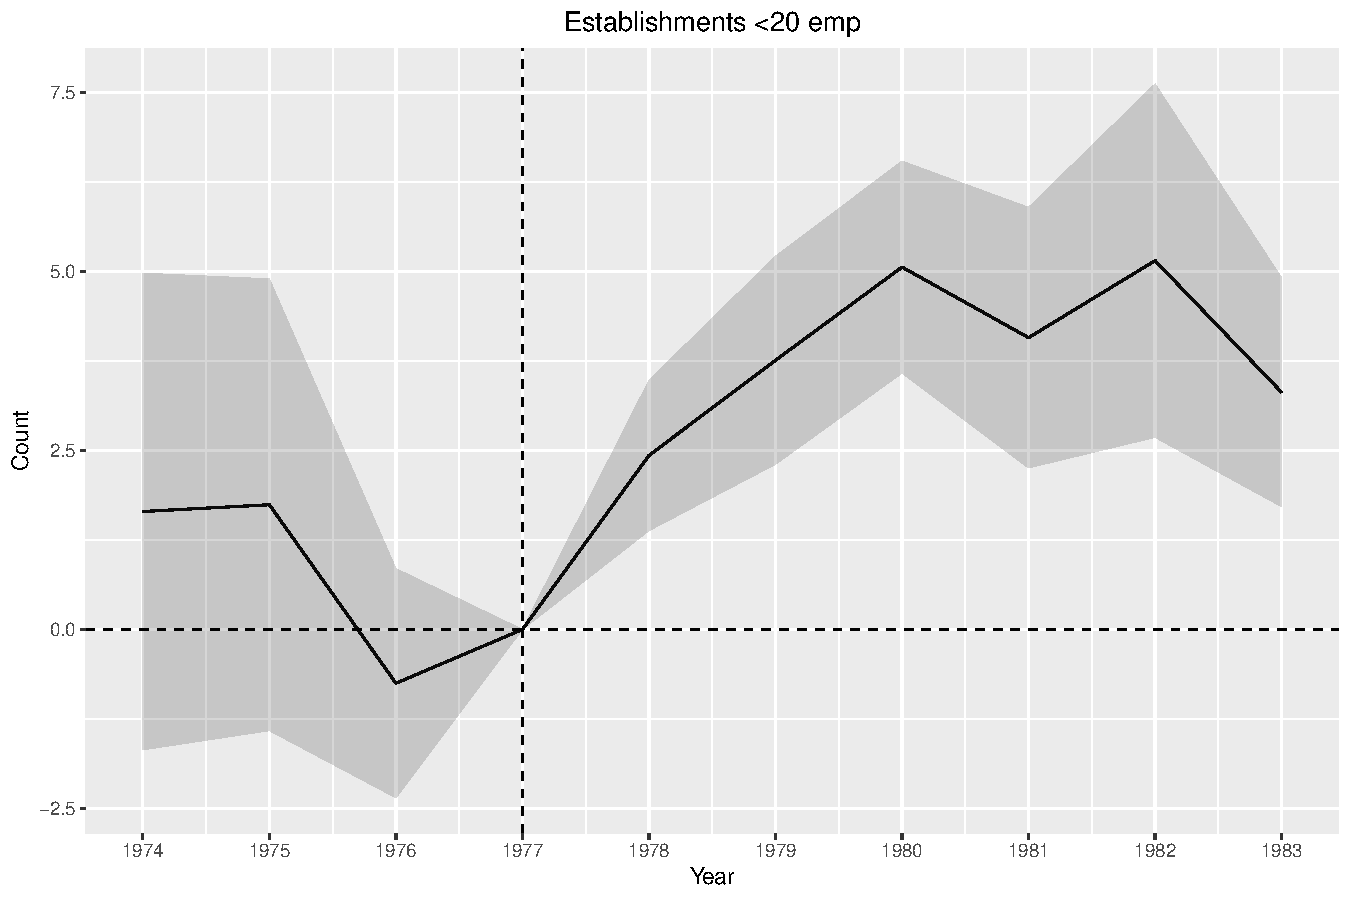
\includegraphics[width=\textwidth]{../Output/Figures/n1_19.pdf}
         \caption{Small Establishments (<20 emp)}
     \end{subfigure}
              \hspace{0.65cm}
         \begin{subfigure}[b]{0.3\textwidth}
         \centering
         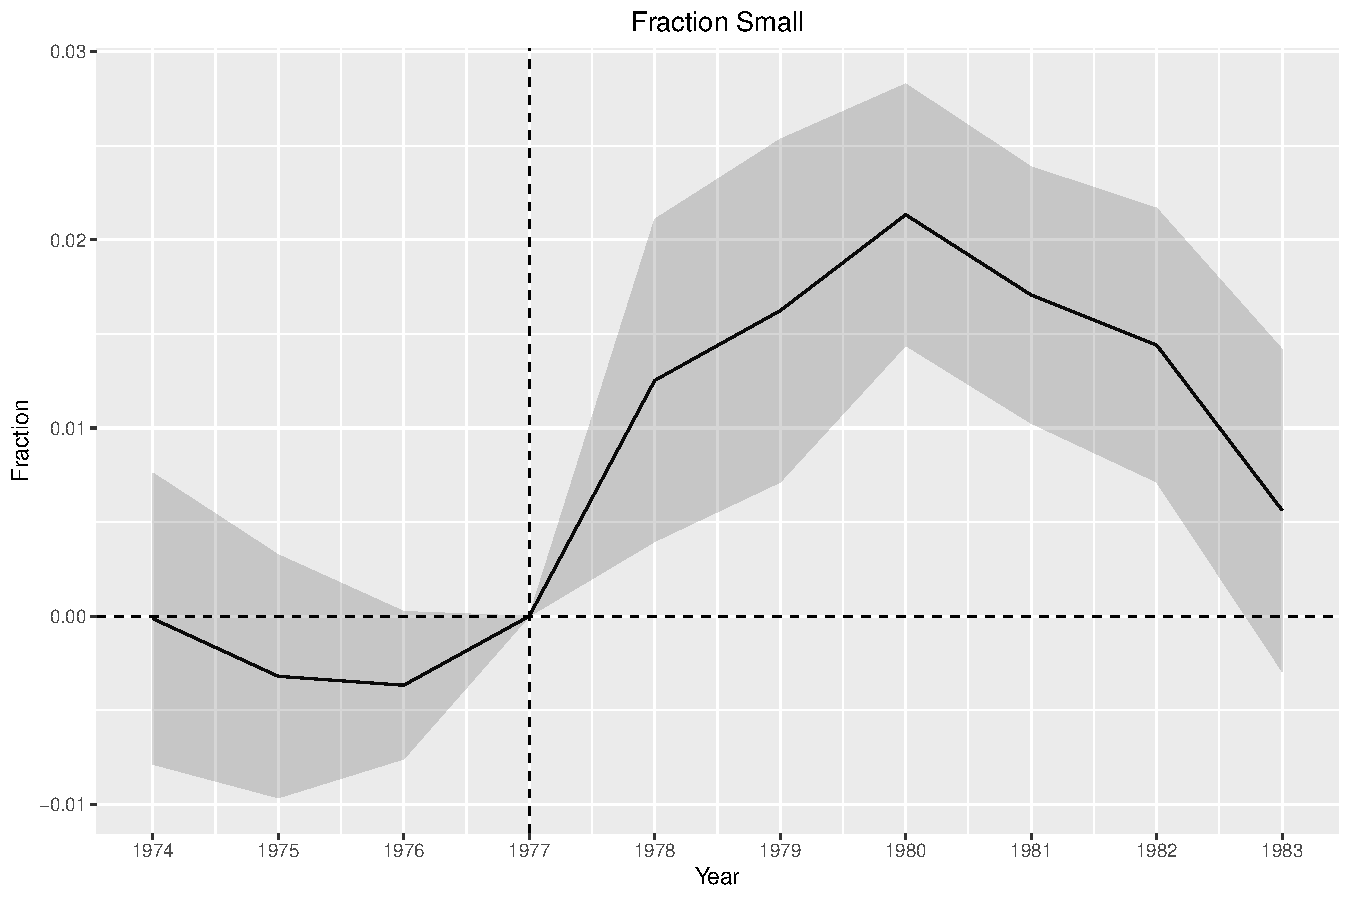
\includegraphics[width=\textwidth]{../Output/Figures/frac_small.pdf}
         \caption{Fraction small}
     \end{subfigure}
        \end{center}
\small \uline{Notes:} This graph shows the results of equation \ref{eq:triple_dif} for number of establishments by 2-digit SIC code-county. Standard errors are clustered by state. The omitted year is 1977, the year before \emph{Marquette}.
 
\end{figure}

As can be seen, there is an economically and statistically significant increase in the number of firms operating in the clothing retail industry in treated states after \emph{Marquette}. The average retail industry in the average county at this time had 91 establishments (see Appendix \ref{tab:summary_cbp}), so the entry of about 4 firms represents nearly a 4\% increase in the number of firms. Although the estimated cost reductions per firm are modest in magnitude (on the order of 2--3\% of marginal cost), the large entry response is consistent with the economics of competitive industries. Entry and exit are threshold decisions: in a competitive industry such as retail, where profit margins are thin, even a small reduction in marginal cost can push many marginal firms from below to above the zero-profit threshold. This is a standard feature of models of entry under competition, such as \cite{hopenhayn_entry_1992} and \cite{melitz_impact_2003}, where the entry margin amplifies small changes in underlying profitability. Furthermore, the firms entering are relatively small, and small firms do not appear to grow to keep the distribution of firm sizes the same -- there is an increase of 2\%, from a mean of 90\%, in the fraction of firms which have less than 20 employees. This is consistent with a channel of cost reduction being economies of scale, which predicts that firms of a smaller scale will benefit more from being able to outsource credit supply functions to large banks. 

\subsection{Accounting Profits}

I calculate the annualized growth in accounting Net Income ("NI") margin over revenue, which I call "Profit growth", as $\mathrm{Profit\,growth}_i = \left(\frac{NI_{i,1983} - NI_{i,1977}}{Revenue_{i,1977}}\right) ^ {1/(1983-1977)}$ to closely follow the decomposition in Equation \ref{eq:decomposition}. I include the 185 firms who have positive net income as of 1977. I use growth rates rather than levels for three reasons. First, differencing eliminates firm-level heterogeneity in baseline profitability, which is substantial across the size distribution of retail firms. Second, parallel trends in profit \emph{growth} is a more plausible identifying assumption than parallel trends in profit \emph{levels}, given the wide cross-sectional variation in firm profitability. Third, the use of growth rates is standard in the firm-level difference-in-differences literature (\cite{beck_finance_2008}). I then estimate the effect of bank credit cards using the cross-sectional analogue of Equation \ref{eq:dif_dif}, where the 2-digit SIC code of firm $i$ is denoted $j$: 

\begin{equation}\label{eq:profits}
\mathrm{Profit\,growth}_{i}= \alpha_{j} + \beta \times Treated_{i} +  \varepsilon_{i}
\end{equation}
 
\begin{table}[!ht]\label{tab:profits}
\caption{Difference-in-Difference of Accounting Profits}\label{tab:profits}


\begingroup
\centering
\begin{tabular}{lc}
   \tabularnewline \midrule \midrule
   Dependent Variable:    & Net Income / Revenue\\  
   Model:                 & (1)\\  
   \midrule
   \emph{Variables}\\
   Treated $\times$ Post  & 0.0091$^{*}$\\   
                          & (0.0054)\\   
   \midrule
   \emph{Fixed-effects}\\
   Year FE                & Yes\\  
   Firm FE                & Yes\\  
   \midrule
   \emph{Fit statistics}\\
   Observations           & 2,000\\  
   R$^2$                  & 0.21338\\  
   Within R$^2$           & 0.00058\\  
   \midrule \midrule
   \multicolumn{2}{l}{\emph{Clustered (Firm FE) standard-errors in parentheses}}\\
   \multicolumn{2}{l}{\emph{Signif. Codes: ***: 0.01, **: 0.05, *: 0.1}}\\
\end{tabular}
\par\endgroup



%Bootstrap these Std Errors
\end{table}

Table \ref{tab:profits} reports the results of estimating Equation \ref{eq:profits}. The point estimate is a 2.1\% increase in profit growth, with a p-value just below 0.1. This analysis suffers from lower power than that of all establishments due to the poor availability of accounting data in the 1970s, but is included for completeness. Nonetheless, these results are at least able to rule out at the 95\% level that the growth in bank credit cards hurt firms by more than 50 basis points of total profits. 

\subsection{Which Firms Adopt Bank Cards?}\label{sec:adoption_firms}

The pattern of which firms choose to adopt bank cards also contains information about the incentives for bank card usage by firms. Recall that there are two main competing explanations: increasing demand or reducing cost. What predictions do these two explanations make about the pattern of adopting firms? To answer this question, I argue (1) geographically concentrated firms have higher cost reduction from accepting cards, and (2) higher market share firms have lower incentive to increase demand. I argue that (1) is true because firms that are diversified across geography can bear the loss of writeoffs at one location more easily if they are diversified against economic shocks in any one specific location. I argue (2) is true because demand is more elastic when market share is lower -- indeed in the nested logit model, price elasticity is $-\alpha p_i \left(1 - s_i\right)$, where $s_i$ is market share.

Which holds true in the data? To answer this question I individually link firms from the Dun \& Bradstreet dataset to manually-collected Yellow Pages records of bank card acceptance using the methodology in Appendix \ref{sec:construction}. This gives me a panel of 2,956 firms in 283 phonebook regions from 1970 to 1985. For each firm, I observe (1) its sales in each year, (2) its 4-digit SIC code, (3) its address, (4) cross-ownership linkages between establishments of the same firm, and (5) whether or not it accepts bank credit cards. I then estimate the following equation using logit regression with fixed effects, reporting average marginal effects:\footnote{I use logit rather than OLS to properly account for the binary nature of the dependent variable. Average marginal effects are computed using the \texttt{marginaleffects} package.}

\begin{equation}\label{eq:adoption_firms}
    A_{ijct} = \alpha_{jct} + \beta_1 \log{\left(SLS_{ijct}\right)} + \beta_2 {Single}_{ijct} + \varepsilon_{ict}
\end{equation}

Where $A_{ict}$ is an indicator variable for whether firm $i$ in 2-digit SIC code $j$ in city $c$ in year $t$ accepts bank cards. $\alpha$ are fixed effects, $SLS$ are sales, and "Single" is an indicator for whether the establishment is the only establishment of the firm (as opposed to one branch of a multi-establishment firm). Errors $\varepsilon$ are assumed to be correlated within 2-digit SIC code $j$. Only firms with sales verified by Dun \& Bradstreet are included in the regression. 18\% of firms in the sample are single-establishment. 

Table \ref{tab:adoption_firms} reports the results of estimating Equation \ref{eq:adoption_firms}. Larger firms, not smaller firms, are more likely to accept bank cards, which is the opposite of what a demand-steering story would predict. Furthermore, single-establishment firms are 4\% more likely to accept cards relative to multi-establishment firms with the same per-establishment sales. Finally, controlling for age has no effect on these coefficients, and I observe that firms older by 1 year on average are about 1\% more likely to accept cards. The results support for the cost-reduction story vis-a-vis the competition story: firms with higher sales, but lower geographic diversity, are more likely to accept bank cards. 

\begin{table}[!ht]
\caption{Which Firms Adopt Bank Cards?}\label{tab:adoption_firms}

\begingroup
\centering
\begin{tabular}{lcc}
   \tabularnewline \midrule \midrule
   Dependent Variable: & \multicolumn{2}{c}{Card acceptance}\\
   Model:                     & (1)            & (2)\\  
   \midrule
   \emph{Variables}\\
   log(Sales)                 & 0.7112$^{***}$ & 0.7243$^{***}$\\   
                              & (0.1500)       & (0.1505)\\   
   Single-establishment       & 0.6874$^{***}$ & 0.7132$^{***}$\\   
                              & (0.2410)       & (0.2308)\\   
   Firm age                   &                & -0.0075\\   
                              &                & (0.0071)\\   
   \midrule
   \emph{Fixed-effects}\\
   Industry $\times$ City FE  & Yes            & Yes\\  
   \midrule
   \emph{Fit statistics}\\
   Observations               & 1,940          & 1,940\\  
   Squared Correlation        & 0.23179        & 0.23384\\  
   Pseudo R$^2$               & 0.24409        & 0.24501\\  
   BIC                        & 1,522.3        & 1,528.6\\  
   \midrule \midrule
   \multicolumn{3}{l}{\emph{Clustered (industry) standard-errors in parentheses}}\\
   \multicolumn{3}{l}{\emph{Signif. Codes: ***: 0.01, **: 0.05, *: 0.1}}\\
\end{tabular}
\par\endgroup

\end{table}


\begin{comment}
    \subsection{Do Bank Cards Change Price Elasticities?}

The prior evidence showing that profitability increases is not supportive of the idea that bank cards intensify competition between merchants. However, to test this more directly, I construct a novel measurement of the intensity of competition between retail firms. The test proceeds in two steps: first, I estimate a proxy for travel costs $t$ based on the differential in sales responses of nearby- vs faraway retail locations to the entry of a new establishment. I find that closer establishments exhibit a stronger decline in sales than further establishments when a new retail establishment in the same narrow (4-digit SIC) industry enters the same town, which is a proxy for $t$ in the Hotelling model. 

The key question is whether the bank card network reduces my proxy for the travel cost $t$. This will be the case, for example, if the travel cost includes a screening cost which only increases with distance for store credit, and not for bank credit -- a reasonable assumption because the bank's comparative advantage is in screening customers irrespective of their community or social ties. This is challenging in the absence of detailed microdata on individual consumers or prices charged by individual merchants. I therefore create a procedure to estimate whether the 1978 supply shock to bank credit card networks reduced a proxy for travel costs $t$, which relies only on data including (1) geographic locations of firms, (2) revenues, (3) competitors, and (4) credit card acceptance decisions of firms, all of which can be identified in the Dun \& Bradstreet database and the Yellow Pages. 

Results Coming Soon 
\end{comment}

\section{Structural Model: Do Cost Reduction or Differentiation Explain the Data?}\label{sec:structural}

The general theoretical framework presented in section \ref{sec:model} is extremely broad and does not make any assumption about the price-setting competitive game between firms, capturing it with a single parameter $\mu$ which summarizes the percentage markup. That model does not allow me to say whether cost changes or differentiation changes appear to be present in light of the data, nor to quantitatively estimate the change in cost that is attributable to a switch to bank credit card technology. In this section, I add structure to the model by building a structural model of price-setting competition between firms, where credit card networks represent a source of product differentiation that can be adjusted counterfactually.

\subsection{Assumptions of the Model}

I use the nested logit framework of \cite{miller_notes_2019} to define the decision problems of consumers and firms, with product differentiation at the group level determined by credit card networks. Specifically, there is a continuum of consumers of measure one indexed by $i$ in each market who observe possible utility from choosing among each discrete option $j$ available in the market. This utility takes the form: 

\begin{equation}\label{eq:utility}
    u_{ij}= \delta_j +\varsigma(g(j)) + \left(1-\sigma\right)\varepsilon_{ij}
\end{equation}

Where the mean utility $\delta_j$ is given by 

\begin{equation}\label{eq:delta}
    \delta_j = \alpha p_j + \xi_j
\end{equation}

Where $p_j$ is the price charged by firm $j$, $\xi_j$ are flexible fixed effects representing the mean quality of each firms' product, $\varsigma(g(j))$ is a product differentiation term indexed by $g(j)$ which is the credit card network used by the firm, and $\varepsilon_{ij}$ is a random shock distributed type-1 extreme value at the individual level. Following \cite{miller_notes_2019}, I further assume that $\varsigma(g(j))$ takes the unique distribution, conditional on $\sigma$, such that $\varsigma(g(j)) + \left(1-\sigma\right)\varepsilon_{ij}$ is also distributed type-1 extreme value. 
I choose this nesting structure because it parsimoniously captures the notion that firms who both accept the same bank credit card must compete more fiercely over the same group of customers. When two firms $j$ and $-j$ are on the same credit card network they share $g(j) = g(-j)$. The consumers that highly value each of their purchase experiences therefore will be the same group of consumers, requiring them to compete more fiercely with each other, but not more fiercely with firms that do not accept the card. $\sigma$ is a free parameter which I estimate subject to $0 < \sigma < 1$ and can flexibly control the degree to which credit card networks actually are a degree of product differentiation between firms. If credit card networks do not actually change the product differentiation between firms, I would recover $\sigma = 0$, if consumers were perfectly segmented by their cardholding choices and never shopped at a store other than one which accepts their preferred card I would recover $\sigma \approx 1$. 
On the supply side, firms optimally set prices to maximize their profits while facing a demand curve which slopes downward due to $\alpha < 0$. Given the model of demand, market shares of each firm are given by 

$$s_j = \frac{exp\left(\frac{\delta_j}{1-\sigma}\right)}{D_g^\sigma \sum_g D_g^{1-\sigma} }$$

Where the $D_g$ for each credit product $g$ is equal to 

$$D_g = \sum_{k \in g} \exp \frac{\delta_k}{1-\sigma}$$

Firm $j$'s first order condition is therefore

$$\left(p_j - c_j\right)^{-1} = \frac{\partial s_j}{\partial p_j} = \frac{\alpha}{1-\sigma}s_j\left(1-\sigma \overline{s}_{j|g}-\left(1-\sigma\right)s_j\right)$$

I close the model with an assumption about cost and quality. In this model, cost and quality are not separately identified -- an increase in product quality of $x$ is equivalent to a cost reduction of $\alpha x$. Therefore I assume that product quality $\xi$ is held constant across counterfactuals, but that cost $c_j$ may change. In particular, the cost $c_j$ is normalised to 1, but changes if the firm accepts the bank credit card. A fraction $f(g)$ of consumers use credit card network $g$. The firms' cost is $1+\zeta f(g(j))$. Therefore the base cost of the industry with all $g$ being singleton networks (single store card networks) is the numeraire of the model.

The notion of consumer ``capture'' in the context of store credit refers to the switching costs created when a consumer opens a store-specific credit account. Once a customer has been screened, approved, and established a credit history with a particular retailer, they face costs of switching to a competitor: the inconvenience of applying for new credit, the potential loss of accumulated credit history, and the familiarity of an established billing relationship. This mechanism is analogous to switching costs in banking relationships (\cite{klemperer_markets_1987}). In the model, this capture effect is embodied in the nesting parameter $\sigma$: when firms share a common payment network (the bank card), the switching cost component of product differentiation is reduced, as consumers can use the same card at any participating merchant.

\subsection{Identifying the Model using Causal Sales Responses}\label{sec:adoption_effects}

\begin{comment}
In this section I estimate the causal effect of bank credit card supply on the sales and survival of retail firms who do and do not accept bank credit cards. These two outcome variables are chosen because they are readily calculable in the Dun \& Bradstreet dataset, and because they are informative about the mechanisms of interest. If firm bank card acceptance is driven by a desire to increase sales among customers who carry bank cards, then an increase in bank card holding among consumers should produce a relative increase in the sales of firms which accept cards. This is the most basic possible prediction of the mechanism. On the other hand, if accepting bank cards is a play to reduce costs, then sales need not change at all -- in fact, the model predicts that their prices will fall, and dollar sales (price times quantity) may even decrease. The lower costs for bank-card-accepting firms will instead show up in higher profitability, which I argue is best approximated by firm survival.     
\end{comment}

To estimate these model, I first construct a sample of establishments which appear in the Yellow Pages as accepting or not accepting bank credit cards (as described in Appendix \ref{sec:construction}) and which appear in 1977 with verified revenue values and survive at least 2 years. For each establishment, I calculate the annual average sales growth $Salesgrowth_i = \left(\log(SLS_{tmax}) - \log(SLS_{1977})\right)/\left(tmax - 1977\right)$.\footnote{$tmax$ is the last year the establishment is observed. I winsorize the growth rate at +100\% per year.} Then, I estimate the effect of the \emph{Marquette} shock in 1978 on these establishments using the estimating equation: 

\begin{equation}\label{eq:adoption_effects}
Salesgrowth_{isj} = \beta_0 Treated_s + \beta_1 Accept_i + \beta_2 Accept_i \times Treated_s + \gamma \log(SLS_{1977}) + \alpha_j + \varepsilon_{isj}
\end{equation}

For outcome variable $Y$ of establishment $i$ in state $s$ and 4-digit SIC-code $j$. State and industry fixed effects are included. $\varepsilon_{isj}$ are errors, clustered at the state level in accordance with the treatment (\cite{abadie_when_2017}). $\beta_0$ represents the treatment effect of bank card growth on establishment' sales who do not initially accept the bank card, and $\beta_2$ is the degree to which this chance in sales is different for accepting establishments.  $\beta_1$ represents the extent to which bank-card-accepting establishments outperform non-bank-card-accepting establishments overall. It is important to stress that the coefficient $\beta_1$ does not have a causal interpretation: as shown in Table \ref{tab:adoption_firms}, there is endogeneity in which establishments choose to accept bank credit cards -- higher-sales establishments are more like to accept. $\beta_1$ is therefore uninformative for estimation of the model. 

\begin{table}[!ht]
\caption{Effects of Bank Card Expansion on Adopting Establishments}\label{tab:adoption_effects}

\begin{tabular}[t]{llrr}
\toprule
industry & acceptance & n & firms\_accepting\\
\midrule
Clothing & 1.5\% & 4513 & 67\\
Furnishing & 0.7\% & 4686 & 34\\
Misc. & 0.6\% & 11982 & 68\\
Auto & 0.5\% & 10154 & 46\\
Department Stores & 0.3\% & 2332 & 7\\
\addlinespace
Hardware & 0.3\% & 3112 & 9\\
Restaurants & 0.1\% & 12794 & 17\\
Food & 0.0\% & 8247 & 2\\
\bottomrule
\end{tabular}

\end{table}

Table \ref{tab:adoption_effects} reports the results of Equation \ref{eq:adoption_effects} estimated at the establishment-level. The most useful of these results for identifying the model is $\beta_2$, the heterogeneity in sales responses to the growth of bank credit cards, which will be crucial for separately identifying the effect of markups from the effect of costs. The intuition behind this is that if bank credit cards reduce markups by easing substitution between firms on the bank credit card network, those already on the network have to lose sales and compress their markups simultaneously. A quantitative model is needed to interpret this evidence because a competing firm reducing their cost (by switching to the bank card network) will already imply some amount of reduction in a firm's sales. The model is therefore needed to quantitatively disentangle how much of the sales response would already be expected by the reduction in cost; any sales reduction beyond that is then explained by the model as tighter competition. 

To build the model, I use data from 252 markets where Yellow Pages data can be merged to Dun \& Bradstreet. I match the median market structure in terms of number of competing firms, realistic heterogeneity in market shares, bank card acceptance, and consumer bank card usage. I then calibrate $\sigma$ and $\zeta$ to match two moments estimated directly from the firm-level sales data around the \emph{Marquette} shock: (i) the average sales response of treated firms, the $Treated\times Post$ coefficient, and (ii) the differential sales response of card-accepting versus non-accepting firms, the $Treated\times Post\times Accept$ coefficient. Both moments, together with their state-clustered sampling covariance, are estimated in a single firm-level regression so that uncertainty propagates jointly through to the structural parameters. %I estimate outside option as time-series average of sales/max sales in each market; then match median market (outside option = 0.08).
I note that, importantly, I modify the standard procedure (\cite{miller_notes_2019}) to correctly match data on sales (Price x Quantity) instead of market shares (Quantity) which the standard method assumes are observed.

\begin{comment}
The estimated causal effect of bank card growth on card-accepting firms is +0.8 years on survival, but -0.02 log points on sales growth. This is consistent with cost-reduction but inconsistent with markup reduction. Indeed, one implication of the model is that if revenue decreases but economic profitability (proxied by survival) increases, this must represent a cost decrease and a markup decrease.      
\end{comment}

\subsection{Calibration Results}

Table \ref{tab:estimation_results} reports the results of calibrating the model by matching moments from the reduced-form causal estimates of the \emph{Marquette} shock on the median retail market in 1978. The price coefficient $\alpha$ is calibrated from the literature rather than estimated; $\sigma$ and $\zeta$ are then identified by matching two moments: the average sales response of treated firms (the $Treated\times Post$ coefficient) and the differential sales response of card-accepting versus non-accepting firms (the $Treated\times Post\times Accept$ coefficient). This is a calibration exercise rather than a full structural estimation in the spirit of BLP, as I match a small number of moments to identify a small number of parameters.\footnote{This distinction is important: the model is used to decompose the observed causal effects into cost and competition components, not to estimate demand primitives from market-level variation. The approach is closer in spirit to Marshall's ``Second Law of Demand,'' as discussed by \cite{melitz_impact_2003}, where elasticities of substitution between firms determine how cost shocks propagate through the industry.} Because the model is exactly identified, it matches both moments exactly, and the mapping from moments to parameters is invertible; I therefore obtain standard errors on $(\sigma,\zeta)$ by the delta method, propagating the (clustered) sampling covariance of the two reduced-form moments through this mapping. My point estimate of $\sigma = 0.017$ (s.e.\ $0.025$) implies that roughly 2\% of the dispersion in consumer tastes across retailers is attributable to their shared acceptance of payment methods, rather than to the products and services the stores themselves offer. To my knowledge this is the first attempt to decompose consumer preferences over retailers into a product-taste component and a payment-method component, and even this seemingly small figure is economically meaningful: it implies that payment networks are a genuine, if secondary, dimension along which consumers choose where to shop. I do not interpret this estimate as ruling out that credit cards shape consumer preferences---rather, the contribution of the structural exercise is to \emph{bound} that channel. Because this is a calibration exercise rather than a strict hypothesis test, I emphasize the point estimate together with its bound: the 95\% confidence interval for $\sigma$ is roughly $[-0.03,\,0.07]$, so the data admit payment methods accounting for as little as essentially none and at most about 7\% of taste dispersion, placing a firm ceiling on the competition-intensifying role of card networks. My point estimate of $\zeta = -0.105$ (s.e.\ $0.055$) implies that, with 37\% bank credit card usage among consumers, the total cost reduction among firms who switch is 3.9\% of marginal cost (s.e.\ $2.0\%$). Because this is a calibration exercise rather than a strict hypothesis test, I emphasize the point estimates and the sign and bound of the effect rather than rejection of a null: the 95\% confidence interval for the cost reduction is roughly $[0.0\%,\,7.8\%]$, so the data bound any cost \emph{increase} from card adoption to essentially zero while admitting cost savings as large as nearly 8\% of marginal cost. Table \ref{tab:sensitivity_alpha} in the Appendix reports the sensitivity of these estimates to the calibrated value of $\alpha$.

\begin{table}[!htp]
\caption{Calibration Results}\label{tab:estimation_results}
    \centering
    \begin{tabular}{lrc}
\multicolumn{3}{c}{\textbf{Parameters}} \\
Parameter & Value & Method \\
\hline
$\alpha$ & $-4$ & Literature \\
$\sigma$ & $0.017$ (0.025) & Matched \\
$\zeta$ & $-0.105$ (0.055) & Matched \\
N Firms & 7 & Observed\\
N Bank Networks & 1 & Observed\\
Top Firm Share & 47\% & Observed\\
Firm Store Card Share & 83\% & Observed\\
Consumer Bank Card Share & 37\% & Observed
\\ \multicolumn{3}{c}{\textbf{Target Moments}} \\
Moment & Model & Data \\
\hline
$\Delta$ Store Card Share & $-20\%$ & $-20\%$ \\
$\Delta$ Bank Card Share & $+5.5\%$ & $+5.5\%$ \\
Avg $\Delta$ Sales ($Treated\times Post$) & $+2\%$ & $+2\%$ (1.8\%) \\
Accept Differential ($\times Accept$) & $-2.2\%$ & $-2.2\%$ (1.1\%)
\end{tabular}

    \\[0.4em] \footnotesize Standard errors in parentheses. For $\sigma$ and $\zeta$ these are delta-method standard errors, propagated from the clustered sampling covariance of the two reduced-form sales moments through the (invertible) moment map.
\end{table}

Is this quantitative value of 3.9\% cost savings reasonable? Consider that the average firm did about 20\% of their sales on store credit in 1980 (Figure \ref{fig:receivables}), so this represents savings of about 20\% of this bill. With merchant discount fees (swipe fees charged to merchants by the card issuer) of about 4\% at time period, that implies that between labor and writeoffs, merchants were losing nearly 25\% of the price of an additional sale by extending credit. While perhaps striking, this number is not obviously too high. Labor costs spent on bookkeepers on bill collectors were 2.5\% in 1980 (Figure \ref{fig:backoffice_retail}), if half of that was actually used on the 20\% of sales that were on credit then that already accounts for over 6\%, implying stores were writing off about 18\% of their receivables. According to the CFPB,\footnote{\cite{consumer_financial_protection_bureau_credit_2022}} private label credit card charge-off rates reached 18\% in 2010. 

Another way to put these estimates into perspective is to use the model to decompose the simulated effect of \emph{Marquette} into price effects due to competition (the network structure of credit card acceptance) vs. costs (the estimated effect of that network structure on costs). To do this, I calculate prices and cost levels for four factual and counter-factual equilibria in Table \ref{tab:counterfactuals} using the structural model. Column (1) is the ``factual'' equilibrium of the un-treated states, and column (2) is the ``factual'' equilibrium of the treated states, the difference being that the usage of bank cards among consumers, and the acceptance of bank cards among retailers, exogenously increased. The markup is the difference between the cost change and the price change. As can be seen from columns (1) and (2), I estimate that the combination of higher bank card use and lower store card use reduced the average cost basis of the retail industry by about 80bp, and further reduced markups by 5bp, creating a total price reduction of 85bp.

Another way to see this effect is to use the model to estimate two new equilibria where only cost changes, or only competition changes, to predict the counterfactual effects of these two changes in isolation. Column (3) calculates the counterfactual equilibrium where the network structure of demand changes by moving the newly-accepting firm into the bank-card nest, so that it must now compete more fiercely with other firms who also accept the bank card, while holding the broad cost structure fixed. In this equilibrium, markups drop by about 6bp through tighter competition. Column (4) calculates the counterfactual equilibrium where costs change, but the network structure of demand is held constant. Average costs decrease by 80bp, while average markups are essentially flat (about $+1$bp), as the cost reduction accumulates at firms with relatively higher market shares and more differentiated products. Overall, this exercise confirms that, quantitatively, cost reduction (80bp) was the dominant force relative to competition intensification (a 6bp markup compression) in this historical episode of bank credit card technology adoption.

\begin{table}[!htp]
\caption{Decomposing the Effect of Bank Cards}\label{tab:counterfactuals}
    \centering
    \begin{tabular}{c|cccc}
Variable & Baseline & Treated & No Cost & Only Cost \\
 & & (Marquette) & Changes & Changes \\
\hline
 & (1) & (2) & (3) & (4) \\
Price Index & 1.24 & -85bp & -23bp & -79bp \\
Cost Index & 0.99 & -80bp & -16bp & -80bp \\
Markup & 0.25 & -5bp & -6bp & +1bp \\
\end{tabular}

    \\[0.4em] \footnotesize Columns report basis-point changes in the average price, cost, and markup index relative to the untreated baseline (1). Column (2) is the full \emph{Marquette} shock; (3) changes only the nesting (competition) structure; (4) changes only costs.
\end{table}

\section{Risk Sharing as a Mechanism for Lower Cost}\label{sec:cost_reduction}

Why might banks have a lower cost to extend credit than firms? In this section I investigate two specific sources of cost reduction in the model: labor efficiency and risk sharing. The most obvious source of cost reduction is that banks administer one account per customer, screening and collecting from them once, rather than ten stores screening and collecting from each customer ten times. Figure \ref{fig:backoffice_retail} reports evidence for labor costs: the share of the retail wage bill paid to bookkeepers and bill collectors has steadily declined from over 4\% in 1940 to less than half a percent in 2020, representing substantial labor savings for retail businesses. But besides the standard explanations of economies of scale and specialization, one interesting and distinctly \emph{financial} reason for cost reduction is that banks are able to diversify credit losses across space and time, unlike small merchants. Since negative demand shocks are strongly correlated with negative household balance sheet shocks, a risk-averse firm will have a high demand for insurance against credit losses specifically in the states of the world where they expect lower demand from their customer base. A national bank, however, has ample opportunities to diversify, and is a natural seller of insurance against shocks. By accepting a bank card, a merchant therefore effectively buys insurance from the bank against credit defaults. 

To test this mechanism, I look at establishment exits, which are a measure of firms' exposure to risk. The cases of the 1975 and 1983 recessions, which occurred before and after \emph{Marquette}, present a good environment to test this mechanism. 1983 in particular was the second-largest recession of the 20th century, with unemployment rates reaching nearly 11\%, as Figure \ref{fig:recessions} shows. I run my difference-in-difference analysis in each year, not just the recession, for completeness, but I am primarily interested in the coefficients on treatment in the year of the recession, 1983. My measure of risk is the exit rate of retail establishments in the Dun and Bradstreet database. I choose this measure rather than change in sales because I am interested in the impact of the combination of lower sales and higher writeoffs at the same time on a measure of firm's real profits and economic decisionmaking, and establishment exit rate is an ideal measure of the real impact of recession risk on firms. 

%Secondly, I look at the rate at which households access the formal bankruptcy system as a measure of household balance sheet distress. The median bankruptcy filer discharges more than \$43,000 in bank credit card debt (\cite{foohey_portraits_2021}). 

\begin{figure}[htp!]
    \caption{Unemployment Rate and Recessions since 1948}\label{fig:recessions}
    \begin{center}
    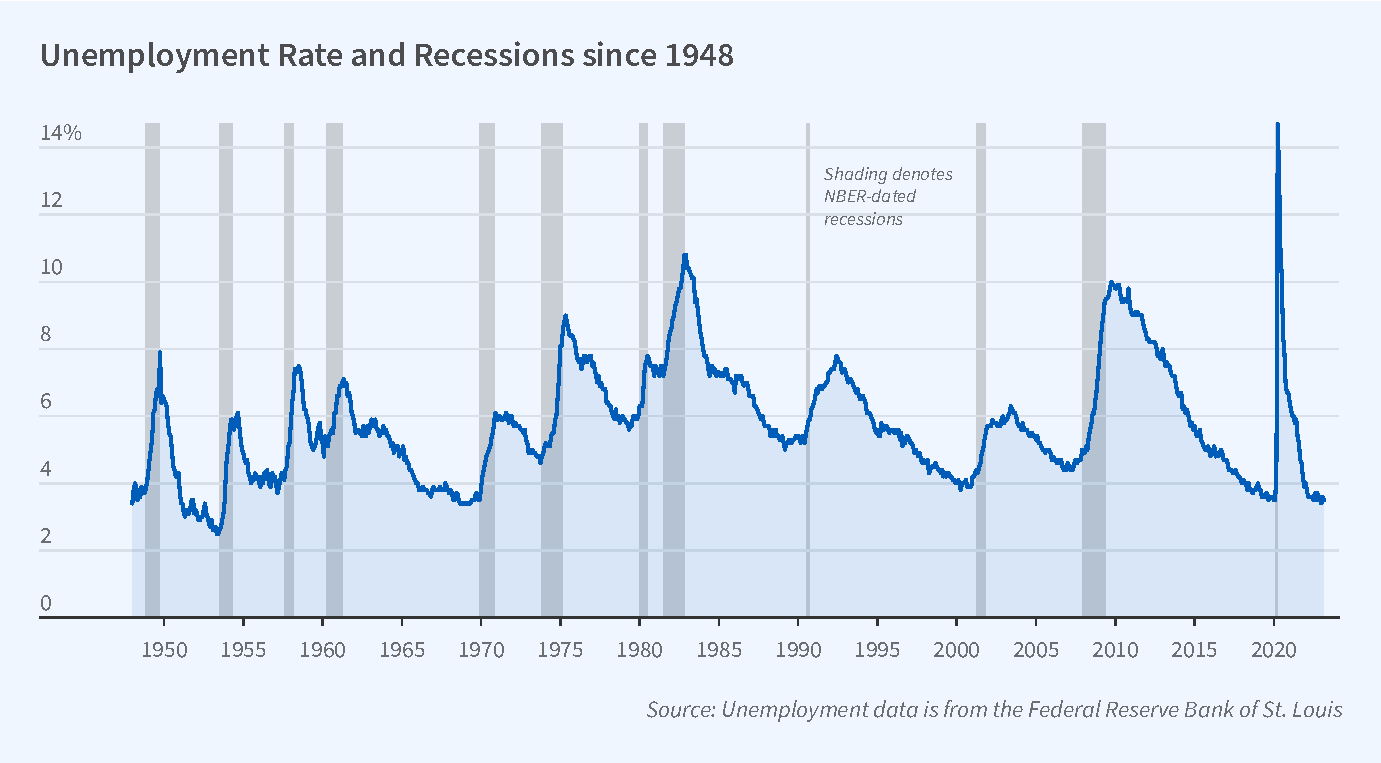
\includegraphics[width = .9\textwidth]{Static/unemployment-rate-and-recessions-since-1948.pdf}
    \end{center}
    \noindent \small \uline{Source:} NBER
\end{figure}

I  use the following analogue of Equation \ref{eq:dif_dif}, with heterogeneity by firm size (single-establishment or multi-establishment. 19\% of establishments are part of a multi-establishment firm). 

\begin{equation}\label{eq:dif-dif-recession}
    P\left[ Exit \right]_{it} = \alpha_{sjt} + \gamma \times \log \left( SLS \right)_{it} + \beta \times Treat_s \times Recession_{t} \times Single_{i} + ...  + \varepsilon_{it}
\end{equation}

Where establishment $i$ is in state $s$ and industry $j$ at time $t$. $Treat_i$ is 1 if the state had a usury limit below 18\% in 1978. $Recession_{t}$ indicator for either 1983 or 1975 depending on the specification, and $Single_i$ is an indicator for single-establishment. ``...'' denote the lower-order interactions, and Std. errors are clustered by state (\cite{abadie_when_2017}). Estimation is with OLS\footnote{Logit performs no better for marginal effects which are the object of interest here, \cite{angrist_mostly_2008}}. The regression is estimated separately on all industries, and on high-adoption industries, defined as 2-digit SIC code 56, clothing retail.  

Table \ref{tab:dif-dif-recession} reports the results of Equation \ref{eq:dif-dif-recession}. Overall, higher-sales establishments are more likely to survive, confirming intuition. During the recession, single-establishments fail at a much higher rate than branches, which also confirms intuition. This holds true regardless of whether the states saw an increase in bank card usage (treatment), and pre- and post-Marquette. The difference appears with the 1983 recession, post-Marquette, when single-establishment firms survived at a 2.3\% higher rate in treated states relative to untreated states. In high adoption industries, this is even higher at 3.2\%. 


\begin{table}[!ht]
\caption{Effect on Retail Establishment Exit Rates in Recessions}\label{tab:dif-dif-recession}

\begingroup
\centering
\begin{tabular}{lcccc}
   \tabularnewline \midrule \midrule
   Dependent Variable: & \multicolumn{4}{c}{Exit rate}\\
   Model:                                              & (1)             & (2)             & (3)             & (4)\\  
   \midrule
   \emph{Variables}\\
   Mean log(Sales)                                     & -0.0092$^{***}$ & -0.0127$^{***}$ & -0.0107$^{***}$ & -0.0155$^{***}$\\   
                                                       & (0.0004)        & (0.0008)        & (0.0005)        & (0.0008)\\   
   Treated $\times$ Single-estab.                      & -0.0006         & -0.0016         & -0.0020         & -0.0041$^{**}$\\   
                                                       & (0.0027)        & (0.0026)        & (0.0015)        & (0.0019)\\   
   Single-estab. $\times$ Recession                    & 0.0459$^{***}$  & 0.0514$^{***}$  & 0.0305$^{***}$  & 0.0159$^{***}$\\   
                                                       & (0.0039)        & (0.0046)        & (0.0033)        & (0.0022)\\   
   Treated $\times$ Recession $\times$ Single-estab.   & -0.0159$^{*}$   & -0.0204$^{**}$  & 0.0003          & 0.0072\\   
                                                       & (0.0081)        & (0.0099)        & (0.0113)        & (0.0084)\\   
   \midrule
   \emph{Fixed-effects}\\
   State $\times$ Industry $\times$ Year FE            & Yes             & Yes             & Yes             & Yes\\  
   \midrule
   \emph{Fit statistics}\\
   Observations                                        & 73,036          & 27,252          & 73,036          & 27,252\\  
   R$^2$                                               & 0.99726         & 0.99720         & 0.99718         & 0.99704\\  
   Within R$^2$                                        & 0.11503         & 0.17114         & 0.08924         & 0.12386\\  
   \midrule \midrule
   \multicolumn{5}{l}{\emph{Clustered (STATE) standard-errors in parentheses}}\\
   \multicolumn{5}{l}{\emph{Signif. Codes: ***: 0.01, **: 0.05, *: 0.1}}\\
\end{tabular}
\par\endgroup


\end{table}

The 1975 recession was also historically significant as seen in Figure \ref{fig:recessions}, but occurred before \emph{Marquette}, making it a good placebo test of the hypothesis that these differences were caused by the growth in bank credit and decline in store credit induced by \emph{Marquette}. No differential response in establishment exit rates are observed in this pre-treatment recession.%\footnote{This analysis suggests another test, which is to examine whether the risk reduction which evidently accrued to firms shows up in the defaults on banks' balance sheets instead using Call Report data. Unfortunately, this analysis is not possible using data which are available to me for reasons discussed in Section \ref{subsec:validity}: Call Report data is organized at the lending institution level, not at the borrower level. It is therefore not possible with public Call Reports to break out bank lending into lending to borrowers in treatment vs. lending to borrowers in control states.} Overall, this evidence is consistent with bank credit cards underwriting a costly source of economic risk to firms. 

\begin{comment}
    \begin{figure}[htp!]
     \centering
     \caption{Difference-in-Difference Estimates of Firm Survival and Household Bankruptcy}\label{fig:dif-dif-recession}
     \begin{subfigure}[b]{0.45\textwidth}\label{fig:exit}
         \centering
         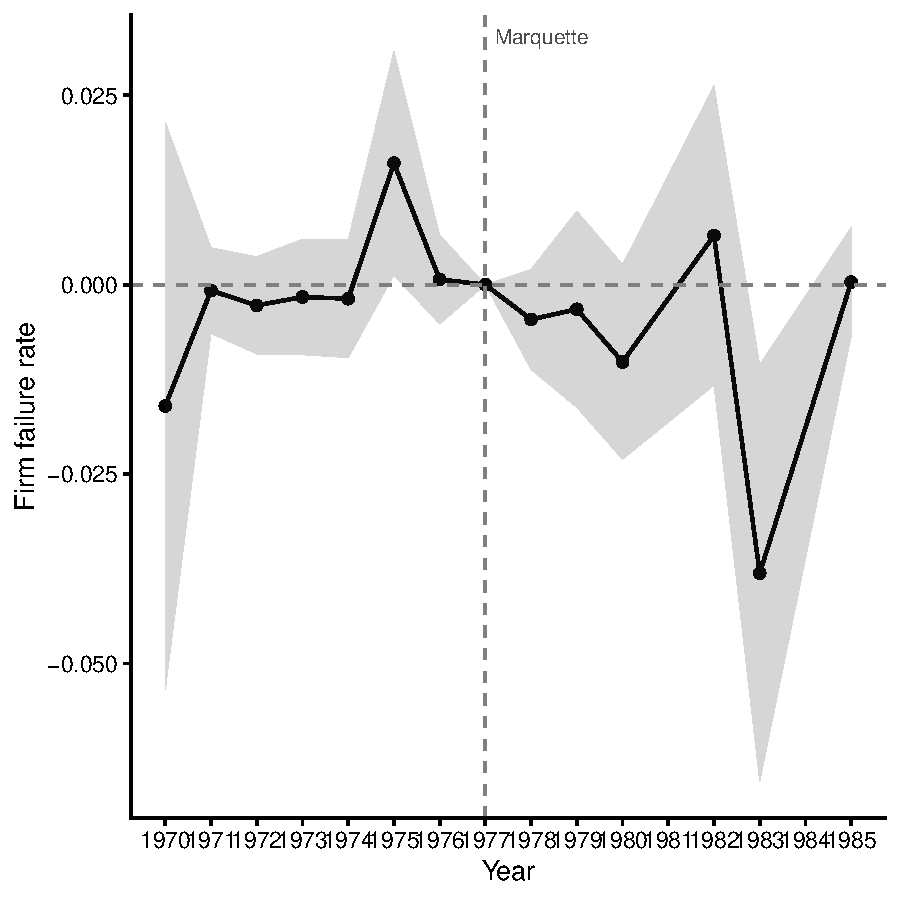
\includegraphics[width=\textwidth]{../Output/Figures/difdif_exit_all.pdf}
         \caption{Firm Exit Rate}
     \end{subfigure}
     \hfill
     \begin{subfigure}[b]{0.45\textwidth}\label{fig:bankruptcy}
         \centering
         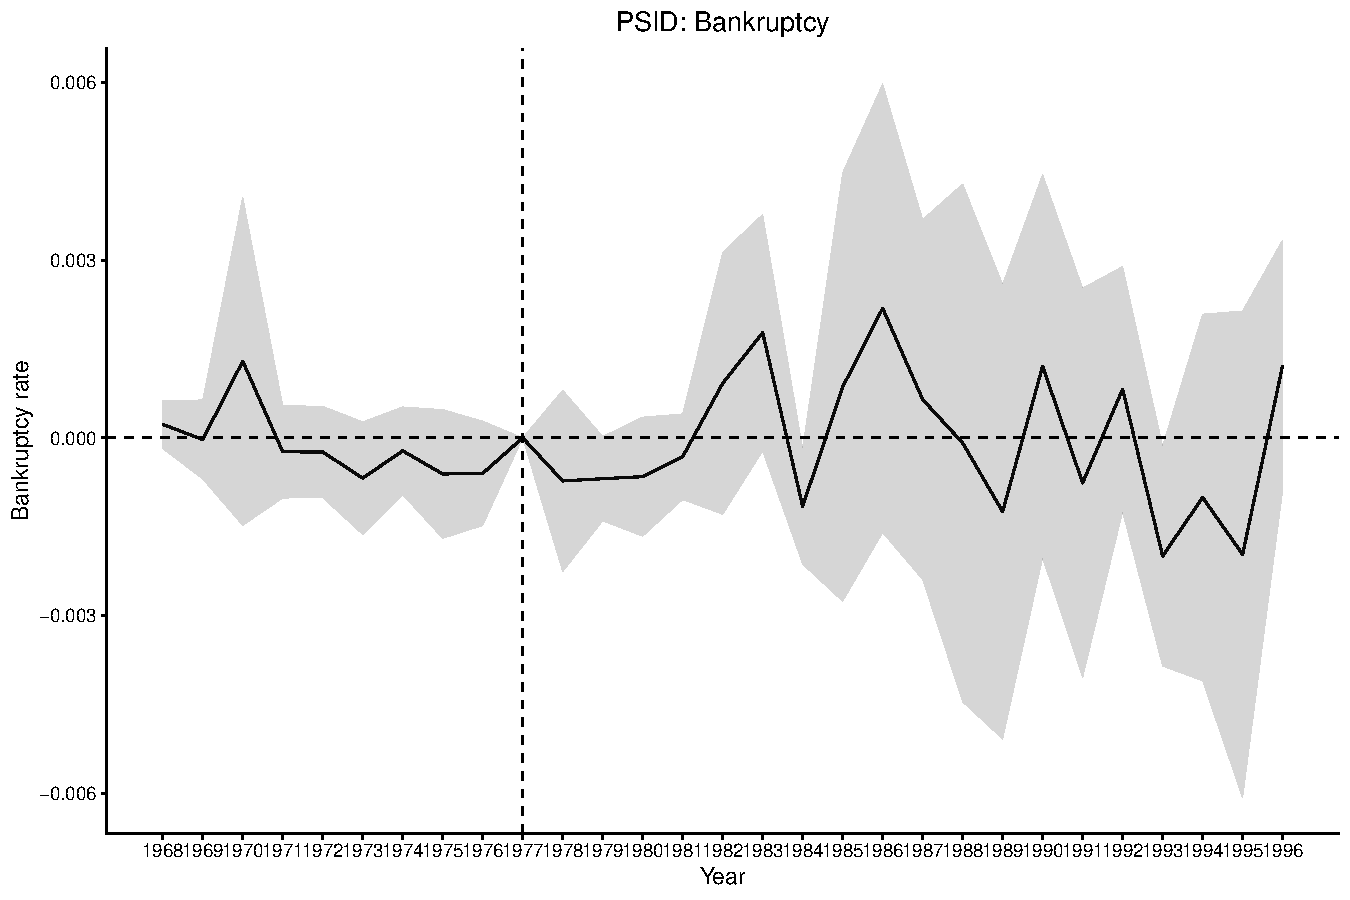
\includegraphics[width=\textwidth]{../Output/Figures/bankruptcy.pdf}
        \caption{Personal Bankruptcy Rate}
     \end{subfigure}
\end{figure}
\end{comment}


\section{Conclusion}\label{sec:conclusion}

Debates over how much lending should occur in an economy, and on what terms, are some of the oldest economic debates in history (\cite{glaeser_neither_1998}). I draw attention to the fact that the technologies used to supply credit matter greatly when answering this question. In particular, specialized credit suppliers such as banks may be superior at such activities for reasons such as economies of scale and the diversification of risk. While merchants complain about paying high fees for something that they view as a simple risk-free transaction, the equivalent of cash, the seeming simplicity of a credit card to the consumer and the merchant belie the complexity and risk of month-to-month lending in a modern global economy with frequent transactions between counterparties without trust. The evidence presented here suggests that merchant discount fees are far less than the cost to perform screening and collection activities in-house, and that small merchants are those who benefit most.

These findings have direct implications for contemporary policy debates over the regulation of interchange fees. The historical evidence suggests that credit card networks created genuine cost savings for merchants, particularly small ones, rather than merely redistributing surplus from merchants to banks. Policymakers evaluating proposals to cap interchange fees should weigh these cost savings against any rents extracted by networks, recognizing that the net effect of credit card infrastructure on merchants has historically been positive (\cite{wang_regulating_2023}). Developing countries should not discount the high labor and risk costs borne by small businesses nor ignore such credit, however difficult to measure, when evaluating costs and benefits of enabling greater consumer financialization in their economies.

\newpage
\singlespace
\bibliography{references}
\newpage


\appendix
\setcounter{table}{0}
\renewcommand{\thetable}{A\arabic{table}}
\setcounter{figure}{0}
\renewcommand{\thefigure}{A\arabic{figure}}

\begin{centering}

\noindent {\Large \bf Appendices}

\end{centering}

\section{Description of Data Sources}\label{sec:data}

\subsection{Survey of Consumer Finance}

To evaluate long-run trends in household revolving credit use, I rely on the Survey of Consumer Finances ("SCF"). One of the most widely-used series' in household finance research, the SCF has been administered continuously since 1947, surveying approximately 3,000-6,000 households per wave in a repeated cross-section. The survey was conducted annually from 1947-1965, 1969-1971, in 1977, and every three years from 1983-2019. I construct detailed series of credit card spending and balances by type of lender from the public SCF files available on the Federal Reserve website and ICPSR.\footnote{The key credit card variables are named x411-x427, x7132, and x7575 in modern releases} 

Table \ref{tab:summary_scf} shows key summary statistics of the SCF data from 1970-2019. The key variables I choose to report are pre-tax income, bank and store credit card spending and balances, store credit balances, primary card interest rate\footnote{The SCF only inquires about the interest rate on the card on which the respondent has the largest balance.}, and auto and mortgage debt balances. Newer SCF releases cover larger samples, so the aggregate statistics are mainly representative of recent years -- accordingly, I separately calculate summary statistics for the pre-1990 period, which is the main period of interest for this study. Overall, monthly bank credit card spending and balances dominate those of store credit cards and store balances, and neither are particularly large compared to auto and mortgage debt balances in the aggregate. Prior to 1990, however, store credit cards and store credit accounts were much closer to those of bank cards. For households in the bottom quartile of income, credit card balances are also a much larger share of their overall borrowing, averaging nearly as much as auto loans. 

\subsection{Public Use Microdata: US Census and PSID}\label{subsec:ipums}

I gather data on key household outcomes from Integrated Public Use Microdata Samples (``IPUMS'') including the US Census and the Panel Study of Income Dynamics, the longest-running representative longitudinal study of U.S. households. I use the US Census to calculate aggregate trends in employment and wages in the retail sector to support the argument that firms choose to adopt bank credit cards in order to reduce marginal costs, particularly labor costs. I show in Appendix Figure \ref{fig:backoffice_retail} that in 1940, over 4\% of the wage bill of the retail industry was paid to bookkeepers and bill collectors, while this fraction has declined smoothly to less than 50 basis points by 2020. These cost-savings are a key ingredient of the model in Section \ref{sec:model}. 

I use the PSID to analyse the prevalence of consumer bankruptcy in Section \ref{sec:substitution}. I restrict attention to household-year observations between 1970 and 1995 which yields 20,823 unique households. The average annual hazard rate of bankruptcy in this time period is 0.18\%, which compares reasonably to the 0.44\% bankruptcy rate in 2020\footnote{544,463 cases among 123.6 million households. Source: UScourts.gov.} given the steady increase in credit card usage since. 

I also rely on the US Census for the Quarterly Financial Reports\footnote{\url{https://www.census.gov/econ/qfr/mmws/current/qfr_pub.pdf}}, which are surveys of firms with over \$50 million which have been collected quarterly since 1947. These data, crucially, include aggregate receivables and revenues by industry. From these data, Figure \ref{fig:receivables} shows the decline in receivables for retail companies which is not mirrored by changes in wholesale companies. 

\subsection{World Bank Global Findex}

To put the United States experience of credit cards in international context, I compare the United States to other countries in the World Bank Global Findex (\cite{global_findex_2021}). This dataset is based on representative samples of over 125,000 households per year in a 123-country panel. The latest public release includes two key variables of interest, store credit usage and credit card ownership, for 329 country-years. 

\subsection{Cost of Personal Borrowing in the United States}

The key independent variable for my main causal analysis is the state of usury regulation in each state in 1977, the year before the Supreme Court \emph{Marquette} decision, which effectively allowed unlimited interest rates on credit cards nation-wide. These data are recorded in the annual volumes Cost of Personal Borrowing in the United States, and have been digitized and generously shared by Rob Seamans (see \cite{chatterji_entrepreneurial_2012}). \cite{chatterji_entrepreneurial_2012} find that state-level usury rates predict transitions to self-employment using the Current Population Survey, particularly so for black men, and specifically in areas with greater historic racial barriers to borrowing and business entry. They conclude that access to credit cards relieved financial constraints and allowed black men to borrow on credit cards and become entrepreneurs. This does not violate my exclusion restriction, because using Equation \ref{eq:triple_dif} I can isolate the effect of credit cards as a transaction mechanism from that of credit cards as a relief to entrepreneurial budget constraints. The most common usury rate in 1977 was 18\%, and all states but New Hampshire had some usury cap. 

\subsection{FRED}

I obtain the rates of inflation and federal funds from the series FPCPITOTLZGUSA and FEDFUNDS from the Federal Reserve Bank of St. Louis Economic Data (``FRED'') at annual frequency. These are used to make a relatively simple point that a usury cap of 18\% was extremely strict in the context of 15\% inflation, and that usury rates below that were below bank marginal cost. 

\subsection{Call Reports}

I obtain Call Reports data from the Federal Reserve Bank of Chicago in order to document trends in credit card lending by origin bank. Using these data, I aggregate total credit card lending by origin bank state and show in section \ref{subsec:validity} that nationwide credit card growth did indeed accelerate after the 1978 \emph{Marquette} decision, and that this boom in consumer lending was indeed driven by banks headquartered in states without usury limits. 

\subsection{Compustat}\label{subsec:compustat}

In order to measure the substitution of bank credit for store credit, I use quarterly data from 1970-1990 on the universe of retail firms (SIC codes 5200-5999) which fit Compustat's inclusion criteria. The key variables are accounts receivable (RECTRQ), total revenue (REVTQ), total assets (ATQ), and net income (NIQ). For each firm, I calculate its ratio of receivables to revenue in each period to measure the amount of credit extended to its customers. Then, I manually match Compustat firms to sales locations in Dun \& Bradstreet with the help of research assistant Sarah Anderson. I then calculate a measure of treatment for each firm as the sales-weighted average treatment intensity across its operating states. I then apply this treatment variable to the difference-in-differences analysis in Section \ref{sec:profits}. There are a total of 195 firms which fit the inclusion criteria for this analysis. The average receivables-to-revenue ratio in the panel is 21.8\%. Table \ref{tab:compustat_summary} in the Appendix reports detailed summary statistics for this sample, including the distribution of geographic treatment exposure. A limitation of the Compustat data is that it covers only large, publicly traded firms and therefore may not be representative of the modal retail establishment, motivating the complementary analysis using County Business Patterns and Dun \& Bradstreet.

\subsection{Dun and Bradstreet}

I obtain data on sales by business establishment from the Dun and Bradstreet establishment-level database, accessed via the Stanford Graduate School of Business library. These data cover retail establishments (SIC codes 5200-5999) across all 50 states from 1970 to 1985, comprising approximately 17 million firm-year observations. For each establishment, the data include annual sales (both verified and estimated), 4-digit SIC industry code, geographic location, year of founding, and linkages to parent firms via the Ultimate DUNS Number. These data are used to identify entry, exit, sales, industry, and location of retail establishments across the United States, and are used in the construction of the data set described in Appendix \ref{sec:construction}. Dun \& Bradstreet, formerly R.G. Dunn \& Company and even earlier as the Mercantile Agency, has been in the business of collecting information and compiling reports assessing the creditworthiness of individuals and businesses in the United States since 1841, making it one of the oldest and deepest registries of information on business establishments that exists (\cite{brennecke_information_2016}). A strength of these data is their comprehensive coverage of small, privately-held establishments that are absent from Compustat. A limitation is that sales figures are sometimes estimated rather than verified, and coverage in the earliest years (1969-1972) may be less complete. The csv data files available via the Stanford Graduate School of Business extend back to 1969.

\subsection{U.S. Telephone Directories}

I collect novel data on firms' credit card acceptance decision using the US Telephone Directory collection from the US Library of Congress.\footnote{Available at https://www.loc.gov/collections/united-states-telephone-directory-collection/}. Appendix \ref{sec:construction} describes the collection of this data, which involves a combination of manual and automated techniques. Banks and firms have a strong incentive to convince customers that their cards are useful and will be accepted at many businesses, and therefore are motivated to make these data as comprehensive as possible.

\begin{figure}[!ht]
     \centering
     \begin{subfigure}[b]{0.45\textwidth}
         \centering
         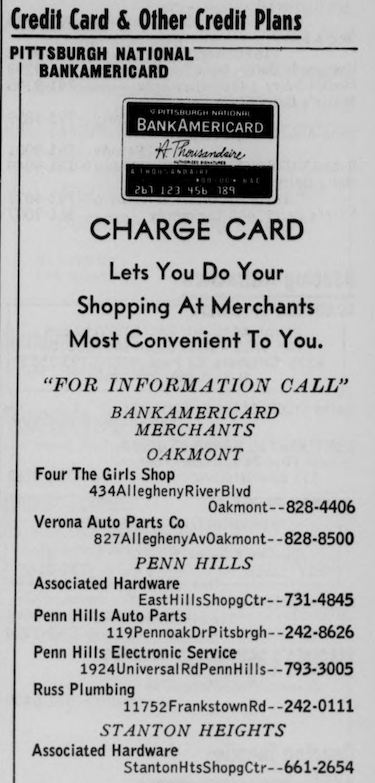
\includegraphics[width=\textwidth]{Static/yellowpages_visa.png}
     \end{subfigure}
     \hfill
     \begin{subfigure}[b]{0.45\textwidth}
         \centering
         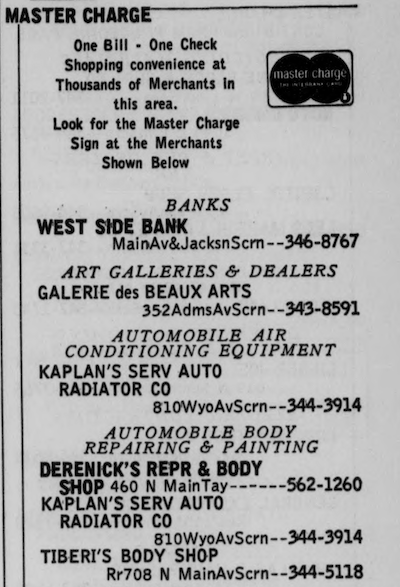
\includegraphics[width=\textwidth]{Static/yellowpages_mc.png}
     \end{subfigure}
        \caption{Examples of USTD Data}
        \label{fig:ustd}
\end{figure}

From these data, I identify the firms most likely to be early adopters of bank cards and their characteristics, which are informative about the mechanisms which incentivize firms to accept bank cards. Table \ref{tab:card_uses} shows the fraction of firms by industry which adopt bank cards in the 1970s, and compares to the primary uses of store and bank cards reported by households in the 1970 SCF. These results motivate the heterogeneity analyses by industry in Section \ref{sec:profits}. These data are also the basis of empirical tests in Sections \ref{sec:adoption_effects} and \ref{sec:adoption_effects} which seek to distinguish between the two major mechanisms of cost-reduction and payment friction reduction. 

\subsection{County Business Patterns}

I collect data on establishment counts across the size distribution of businesses from the US Census' County Business Patterns. These data available are available at an annual frequency since 1946 (\cite{eckert_early_2022}). These data are suitable for examining heterogeneous effects across the size distribution of firms, and aggregate net entry of firms which I argue is a sufficient statistic for economic profits. I aggregate data by year, county, and 2-digit SIC code. Of particular interest is the clothing retail industry, where I hypothesize that the effect of bank credit cards should be apparent, if it exists. As Table \ref{tab:card_uses} shows, clothing was the predominant use of both store and bank credit cards as of 1970. The clothing retail industry is characterised by a larger number of establishments, but fewer total employees, than other similarly-defined industries, indicating a larger fraction of smaller businesses. The second panel of Table \ref{tab:card_uses} is compiled from the Survey of Consumer Finance. For each customer, I sort them into primary bank card or primary store card users based on which card (if either is present) they report spending a higher dollar value on, and then categorize them by their reported primary use of the card. 

\begin{table}[!ht] 
\newcolumntype{C}{>{\centering\arraybackslash}X}
%\begin{center}
\caption{Usage of Bank Cards Across Industries, 1970-1977}\label{tab:card_uses}
%\vspace*{-0.5cm}
\resizebox{.55\textwidth}{!}{\begin{tabular}[t]{llrr}
\toprule
industry & acceptance & n & firms\_accepting\\
\midrule
Clothing & 1.5\% & 4513 & 67\\
Furnishing & 0.7\% & 4686 & 34\\
Misc. & 0.6\% & 11982 & 68\\
Auto & 0.5\% & 10154 & 46\\
Department Stores & 0.3\% & 2332 & 7\\
\addlinespace
Hardware & 0.3\% & 3112 & 9\\
Restaurants & 0.1\% & 12794 & 17\\
Food & 0.0\% & 8247 & 2\\
\bottomrule
\end{tabular}
}
\quad
\resizebox{.45\textwidth}{!}{\begin{tabular}[t]{lll}
\toprule
Card use & Store cards & Bank cards\\
\midrule
Clothing & 84\% & 54\%\\
Appliances & 15\% & 9\%\\
Misc. & 15\% & 38\%\\
Household goods & 14\% & 5\%\\
Recreation items & 8\% & 5\%\\
\addlinespace
Hardware & 5\% & 5\%\\
Furniture & 4\% & 10\%\\
Travel & 0\% & 27\%\\
\bottomrule
\end{tabular}
}
%\end{center}
\uline{Notes:} The first panel describes the fraction of firms across (2-digit SIC code) industries which accept bank credit cards in the US Telephone Directories data. Construction of these data using Dun \& Bradstreet and the US Telephone Directories is described in Appendix \ref{sec:construction}. The second panel describes the fraction of consumers in the Survey of Consumer Finance who identify each given use as their ``primary use'' of store credit cards and bank credit cards. 
\end{table}

\newpage 

\section{US Telephone Directory Data Collection}\label{sec:construction}

\textbf{Phonebook coverage:}
The Dun and Bradstreet (D\&B) database was filtered for the states and years covered by the selected phonebooks, resulting in a dataset of 1,974,721 company-years which could conceivably have appeared in phonebooks. The index sections of each phonebook was manually inspected to generate a list of municipalities covered by each phonebook; the list of municipalities for each phonebook area was not found to vary across years. A merge was performed between the list of localities and the D\&B dataset, using a concatenated city-state merge index. This generated a binary indicator for each D\&B company-year, representing whether or not the company-year is geographically and temporally covered by any of the selected phonebooks. 141,119 (7.2\%) company-years were found to be covered by at least one phonebook. Of the 418 municipalities covered by the phonebooks, 281 (67.6\%) were not represented by any company-years in the D\&B dataset. This is justified by the fact that the phonebook municipality listings contain sub-municipality-level locations, including bodies of water and airports. These locations are all within municipalities listed in both the phonebooks and D\&B, such that they are redundant. Furthermore, some municipalities listed in the phonebooks are very small settlements (population <1,000) that are unlikely to have any commercial establishments.

\textbf{Company matching:}
Individual companies listed under the “Credit Card” portion of each phonebook’s Yellow Pages were manually transcribed to create a dataset of 510 company-years. Each of these company-years represent a merchant that accepted interoperable credit cards in that given year. Other listings pertaining to credit (credit unions, credit reporting agencies, branches of the credit-offering bank, credit card supply or technology companies) were excluded. The phonebook listings are assumed to be a nearly exhaustive list of merchants who accepted credit cards, as both credit card companies and merchants have strong economic incentives to publicize their offerings. Only one credit card plan, Cap Charge Account Plan, noted that the phonebook listing was a partial member list; this plan only appeared in one phonebook. Information represented in the dataset of merchants includes the company’s name, phone number, whether the listing was in bold or large font (presumed to represent paid marketing), the industry / sector the company was listed under, and the credit card plan in which it participated. 
This list of credit-card-accepting merchants was then merged with D\&B dataset to identify which D\&B-listed company-years accepted credit cards. The initial merge used a concatenated year-phone number merge index, where the phone number used was the last seven digits of the phone number provided. This was done to remove noise from area codes or other phone dialing prefixes that sometimes appeared in the D\&B dataset. From this merge, 366 (72\%) company-years from the phonebook data were matched with a record in the D\&B dataset. Manual comparisons of company names confirmed that the records were all correctly matched. The remaining 142 merchant-years were manually matched with D\&B records based on company names, street addresses, and industries, yielding another 47 confident matches. Ultimately, 81.3\% of the merchant-year observations in phonebooks were matched with a D\&B record. The remainder likely did not have a match because the merchant-year predated D\&B’s database (starting in 1970), or D\&B did not record the business as operational in the corresponding year. Finally, the matching phonebook records were merged back into the D\&B database. A total of 410 firms were found to have a matching phonebook listing under a card-accepting merchant. Finally, the D\&B dataset was filtered to only include cities, 4-digit SIC codes, and years in which at least one firm was found that is confirmed to accept the bank credit card, resulting in a population of 2,956 firms from 1970 through 1977. 1,177 of these firms exist as of 1977, i.e. at the time of the \emph{Marquette} shock, of which 525 have verified sales data. 

Company matching was performed by research assistant Sarah Anderson. I (Joseph Hall) specified the procedure, audited a random subsample of results, and accept responsibility for any remaining errors.

\begin{figure}[H]
 \caption{USTD Coverage Over Time}\label{fig:books_by_year}
 \vspace{-0.25cm}
 \begin{center}
  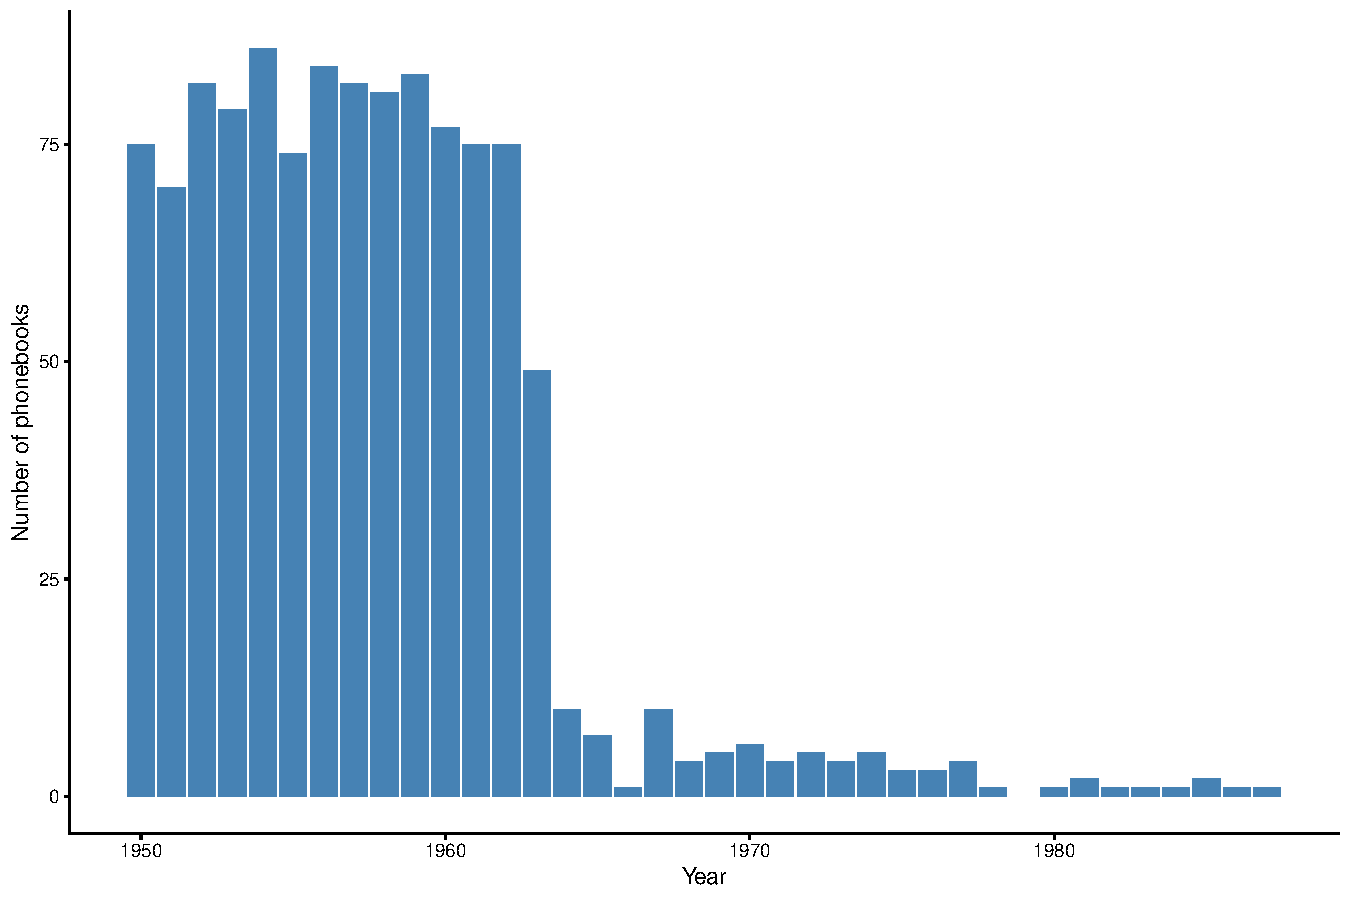
\includegraphics[width=.9\textwidth]{../Output/Figures/books_by_year.pdf}
  \end{center}
\end{figure}
\vspace{-0.5cm}
\noindent \small \uline{Notes:} This figure shows the number of phone books available from the U.S. Telephone Directories collection of the Library of Congress by year since 1950, categorized by state. 

\begin{figure}[H]
 \caption{USTD Coverage and Bank Card Introduction Dates Across US Counties}\label{fig:books_by_county}
 \vspace{-0.25cm}
 \begin{center}
  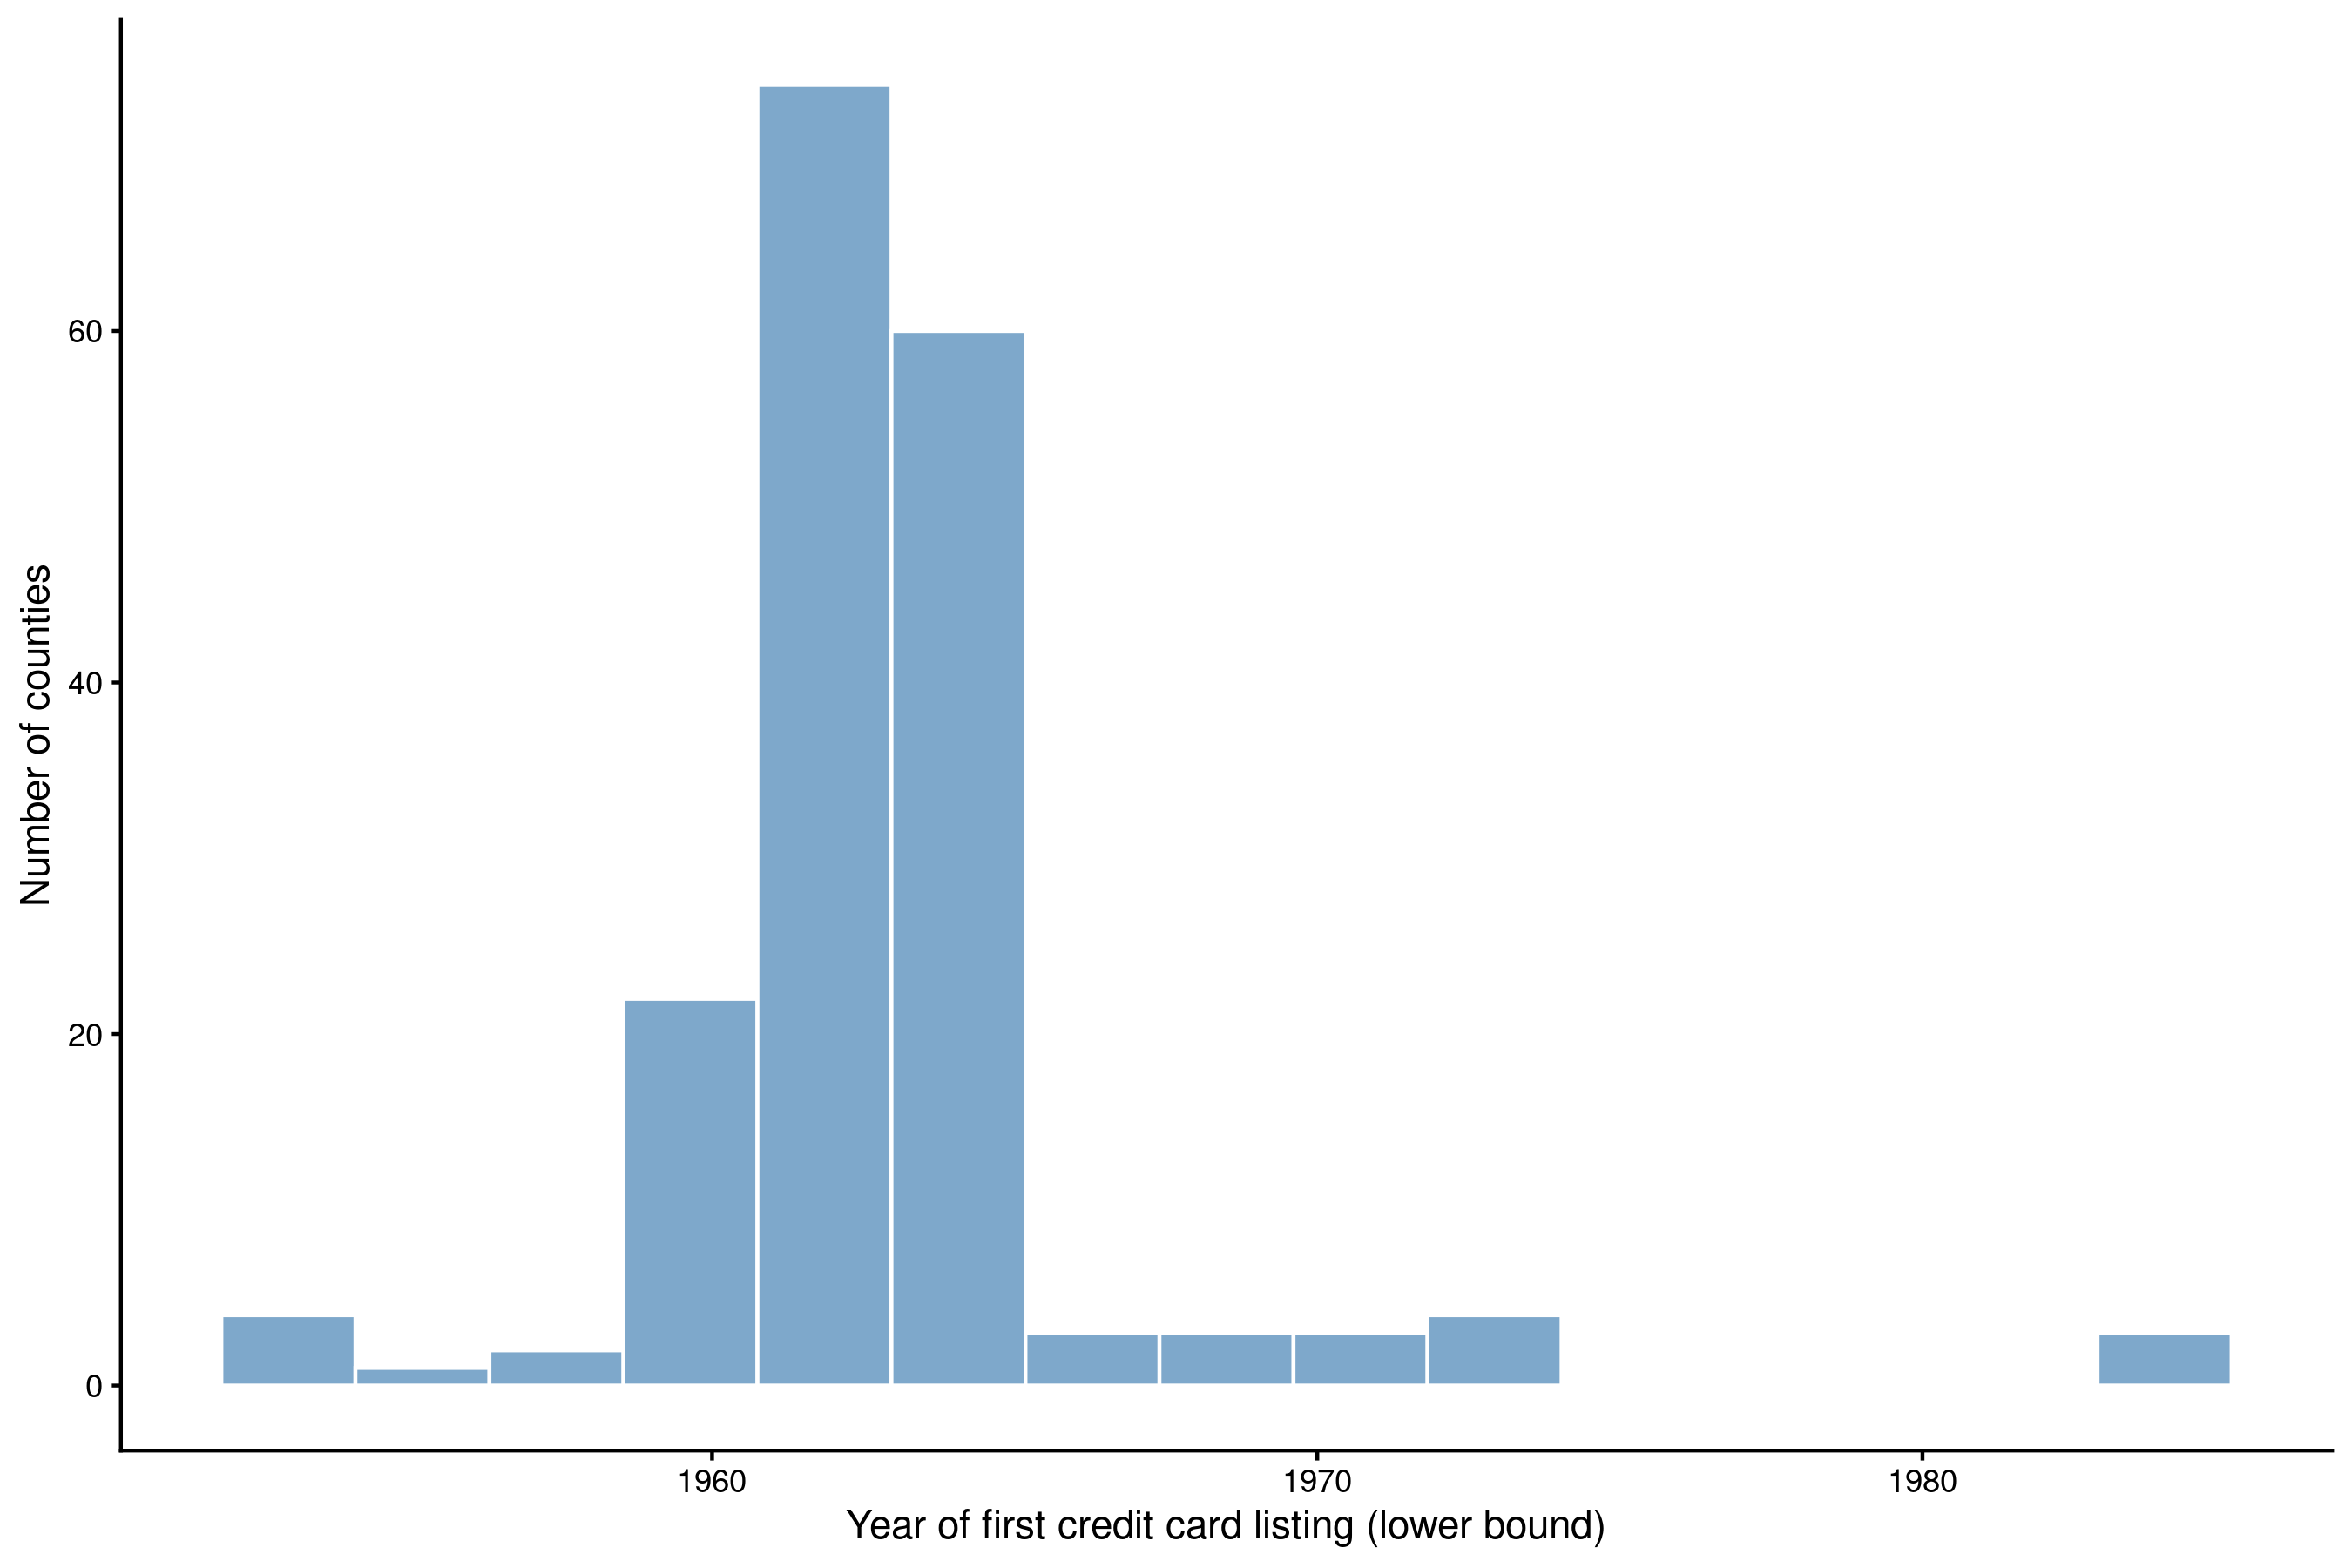
\includegraphics[width=.9\textwidth]{../Output/Figures/intro_lb.png}
  \end{center}
  \noindent \small \uline{Notes:} Counties included in the USTD Collection are marked in shades of blue according to the lower bound of possible introduction dates of bank credit cards. 
\end{figure}
\vspace{-0.5cm}

\begin{table}
\textbf{Representativeness of Yellow Pages Sample}
\centering
\begin{tabular}[t]{lrr}
\toprule
Variable & In Sample & Not In Sample\\
\midrule
Avg Employment ('000) & 407 & 17 \\
Avg Establishments & 26,076 & 1,285 \\
Avg Retail Establishments & 5,897 & 416 \\
Total Employment (M) & 33 & 49 \\
Total Establishments ('000) & 2,112 & 3,598 \\
Counties & 81 & 2,800 \\
\bottomrule
\end{tabular}

\newline
\noindent \small \uline{Notes:} The table compares counties included vs. excluded from the US Telephone Directories Yellow Pages collection. Sampled counties are identified by matching the USTD collection to County Business Patterns geography via the location crosswalk keyed to the 1970 CBP vintage; figures are therefore reported as of 1970. The source of employment and establishment statistics is the County Business Patterns dataset.
\end{table}

\begin{table}[H]
\caption{Firm Characteristics by Phonebook Coverage and Card Acceptance}\label{tab:yp_representativeness}
\centering
\begin{tabular}[t]{lrrr}
\toprule
Group & Mean log(Sales) & Frac. single-estab. & N\\
\midrule
In phonebook area & 11.35 & 0.901 & 109005\\
Not in phonebook area & 11.60 & 0.900 & 1318974\\
Does not accept & 11.35 & 0.901 & 108684\\
Accepts cards & 12.11 & 0.835 & 321\\
\bottomrule
\end{tabular}

\newline
\noindent \small \uline{Notes:} This table compares firm characteristics across phonebook coverage status and card acceptance. ``In phonebook area'' restricts to firm-years in municipalities covered by the USTD collection. ``Accepts cards'' and ``Does not accept'' further restrict to competitive markets (at least one card-accepting firm per SIC-city-year cell).
\end{table}

\subsection*{The US Telephone Directory Corpus as a Research Resource}

The credit card listings used above are the visible output of a much larger digitization effort that I make publicly available as a stand-alone research resource. The phonebook scans in the Library of Congress US Telephone Directories collection are in the public domain; I had them processed by optical character recognition (OCR) and assembled the output into a machine-readable corpus, organized in two layers. The richer layer comprises 110 merged, book-level files in which each word carries a page assignment, a bounding box, and an automated ``category header'' flag; these books contain roughly 3.7 million OCR'd words and 17,995 distinct Yellow Pages category headings. Adding a second, page-level layer yields a combined corpus of 168 phonebooks covering five states, 44 cities, and the years 1950--1978, with approximately 2.1 million business listings (text entries carrying a telephone number) and 49{,}447 unique category headings. Table \ref{tab:ocr_corpus} summarizes the corpus, and Figure \ref{fig:ocr_corpus} shows its coverage by year alongside the diffusion of dedicated ``Credit Card'' directory sections across cities.

\begin{table}[H]
\caption{The US Telephone Directory OCR Corpus}\label{tab:ocr_corpus}
\centering
\begin{tabular}[t]{ll}
\toprule
 & \\
\midrule
Phonebooks in OCR corpus & 168\\
--- from merged book-level files & 63\\
--- from page-level files (new) & 105\\
Total pages scanned & 41,619\\
Business listings (with phone numbers) & 2,074,980\\
\addlinespace
Unique business categories & 49,447\\
Books with credit card sections & 13\\
States covered & 5\\
Cities covered & 44\\
Year range & 1950-1978\\
\bottomrule
\end{tabular}

\newline
\noindent \small \uline{Notes:} Summary of the machine-readable phonebook corpus constructed from the Library of Congress US Telephone Directories collection. ``Business listings'' are OCR text entries containing a telephone number. ``Books with credit card sections'' counts phonebooks in which the automated detector identifies a dedicated ``Credit Card \& Other Credit Plans'' category. The merged book-level files additionally carry word-level bounding boxes and category-header flags; the page-level files provide raw OCR text only.
\end{table}

\begin{figure}[H]
\caption{Phonebook Corpus: Coverage and Credit-Section Diffusion}\label{fig:ocr_corpus}
\centering
\begin{subfigure}[b]{0.49\textwidth}\centering
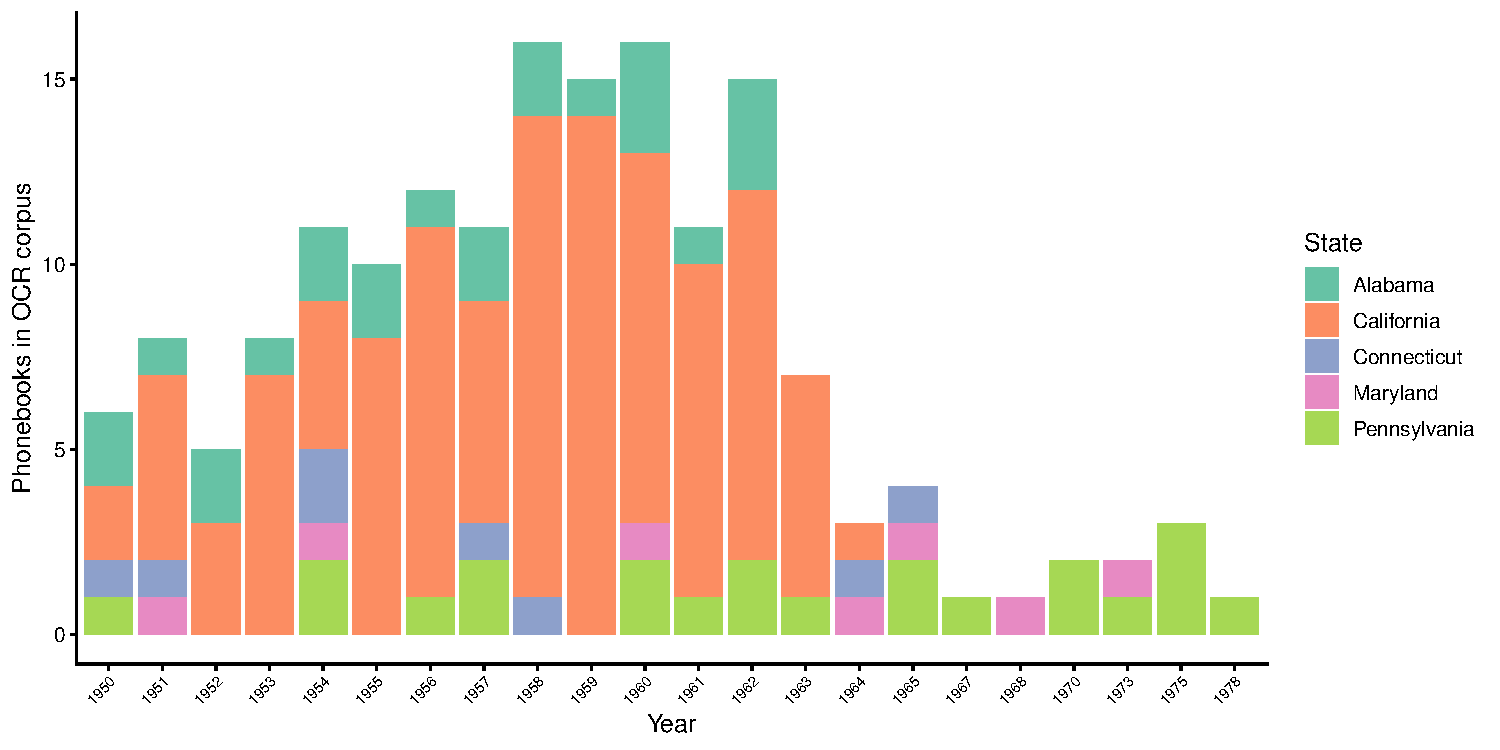
\includegraphics[width=\textwidth]{../Output/Figures/yp_review/A_full_corpus_by_year.pdf}
\caption{Phonebooks by state and year}
\end{subfigure}\hfill
\begin{subfigure}[b]{0.49\textwidth}\centering
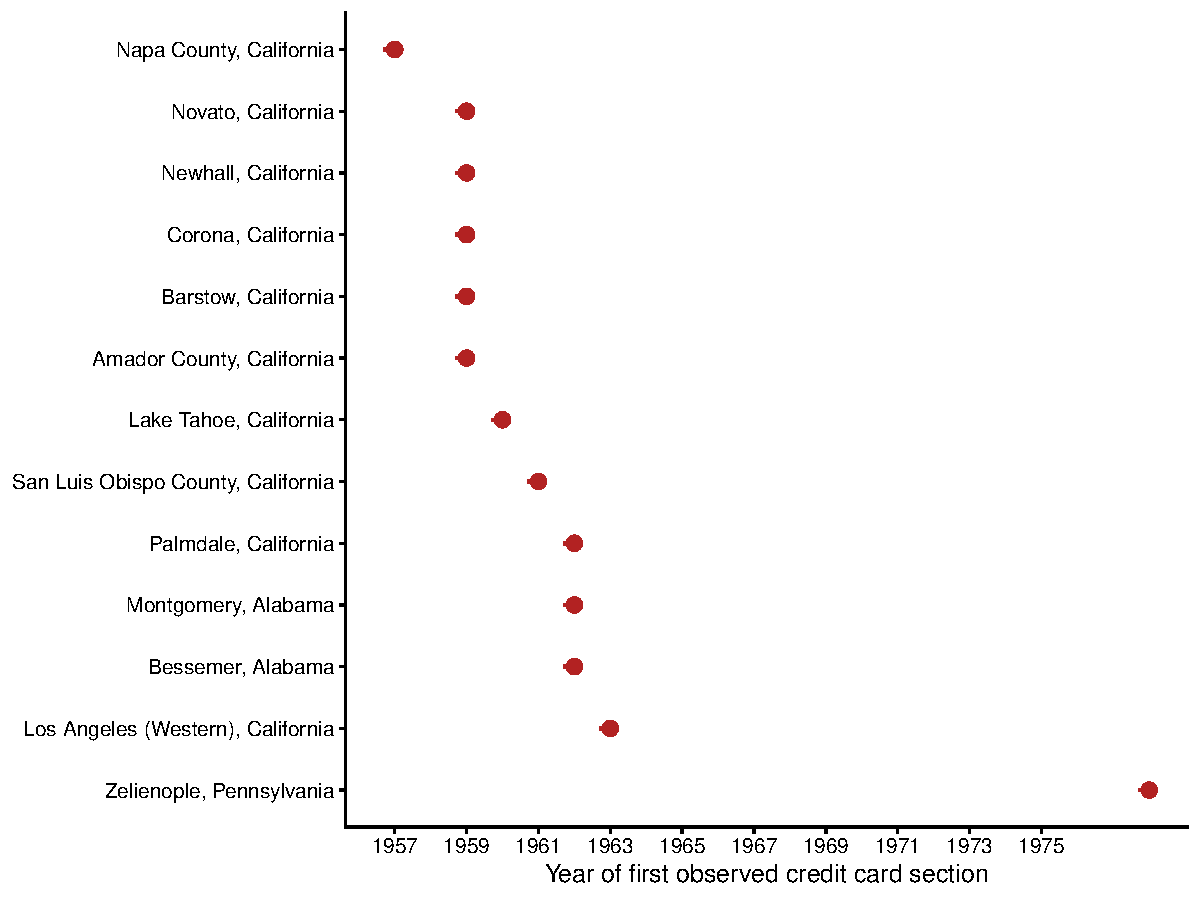
\includegraphics[width=\textwidth]{../Output/Figures/yp_review/D_credit_section_intro.pdf}
\caption{First appearance of a ``Credit Card'' section}
\end{subfigure}
\end{figure}
\vspace{-0.25cm}

\noindent The full corpus, the hand-transcribed credit card acceptance records, a data dictionary, and the code that produces every figure and table in this section are archived on Zenodo at \href{https://doi.org/10.5281/zenodo.20513427}{\texttt{doi.org/10.5281/zenodo.20513427}} and mirrored in the paper's public replication repository. Because the corpus derives from public-domain materials, it may be freely reused; the proprietary Dun \& Bradstreet records used to attach establishment sales are not redistributed and must be licensed separately.

\newpage

\section{Summary Statistics}\label{sec:summary-stats}

\begin{table}
\centering
\caption{Summary Statistics: Survey of Consumer Finances}
\centering
\begin{tabular}[t]{lrrr}
\toprule
Variable & Mean & SD & N\\
\midrule
income & 620093.68 & 5259192.50 & 281982\\
has\_card & 0.77 & 0.42 & 282652\\
has\_bank\_card & 0.72 & 0.45 & 279823\\
has\_store\_card & 0.50 & 0.50 & 279823\\
card\_spend & 3012.49 & 18244.66 & 275548\\
\addlinespace
card\_bal & 1952.76 & 7058.71 & 280873\\
\bottomrule
\end{tabular}
\end{table}

\label{tab:summary_scf}
\noindent \small \uline{Notes:} This table reports summary statistics for the Survey of Consumer Finance data from 1970-2019. Means are weighted by SCF sample weights. For surveys with multiple imputation, only the first implicate is used. Counts reflect non-missing data, which change between variables due to either invalid responses or changes in the composition of questions in the survey over time. Panel 3, ``Bottom Quartile by Income'' includes respondents in the bottom quartile of income for their respective survey year. Dollar amounts are nominal, i.e. not inflation-adjusted.

\begin{figure}[H]
 \caption{Credit Card Interest Rates}\label{fig:card_rates}
 \vspace{-0.25cm}
 \begin{center}
  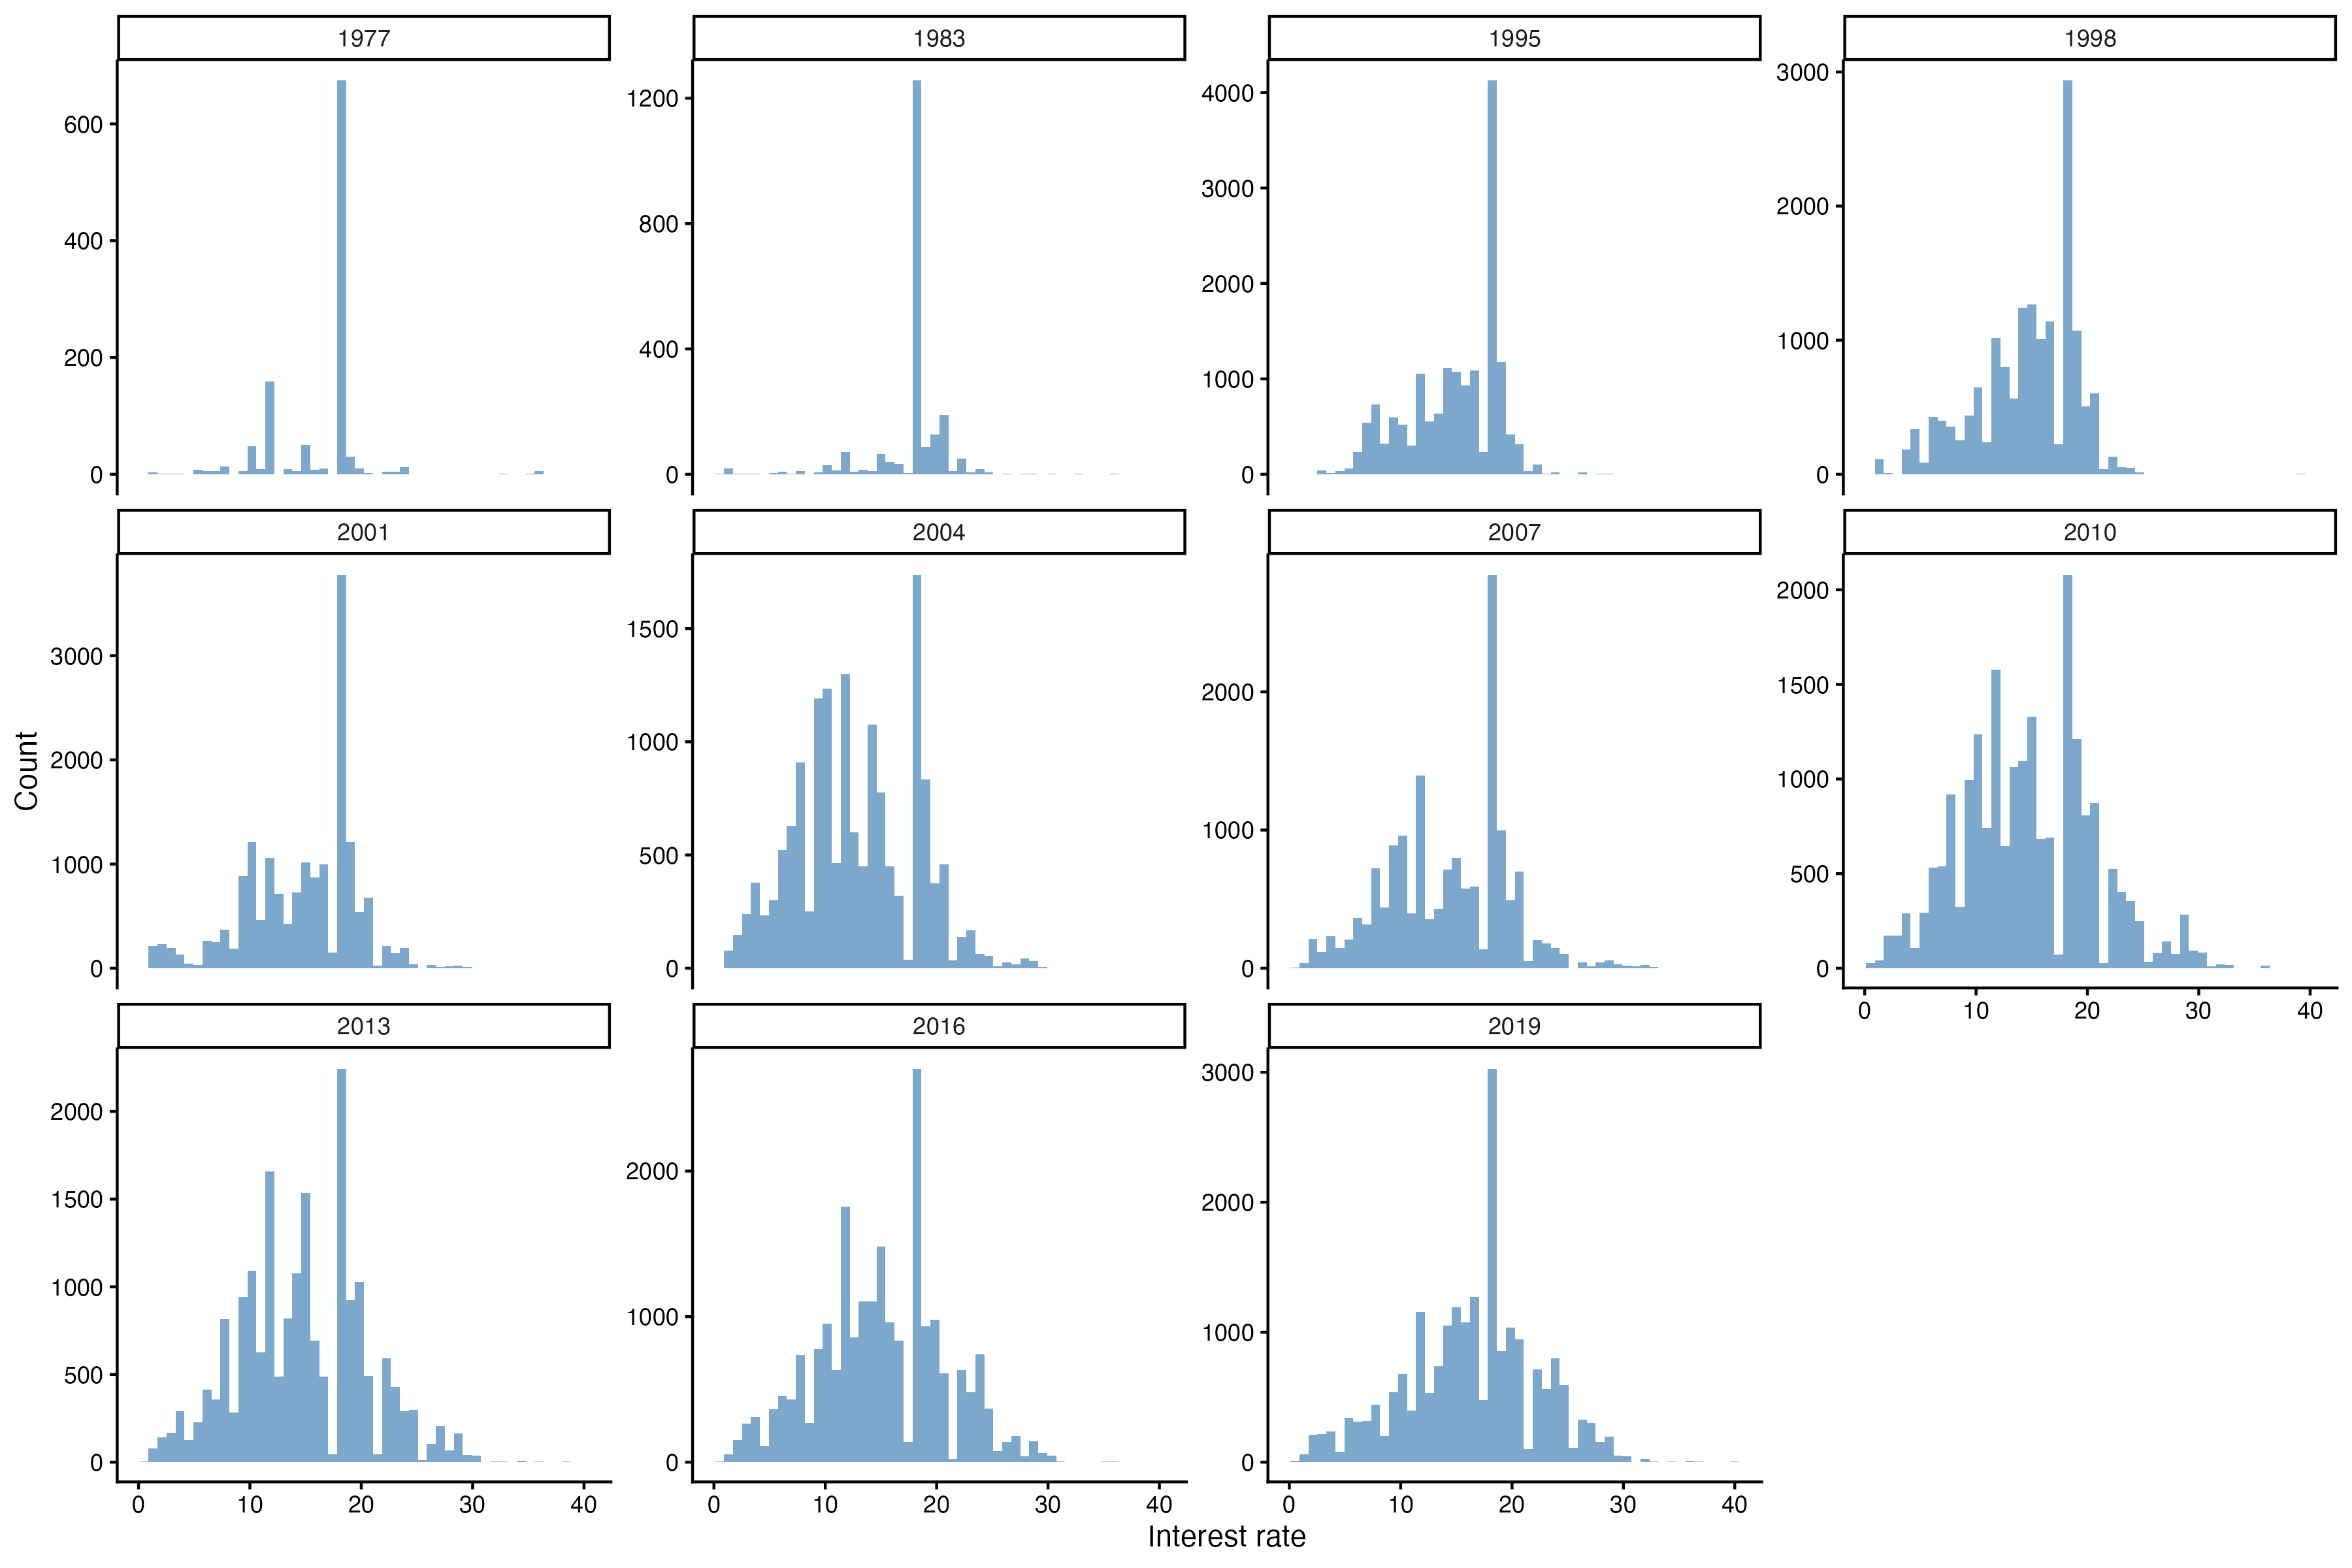
\includegraphics[width=.8\textwidth]{../Output/Figures/rates_all.png}
  \end{center}
  \noindent \small \uline{Notes:} The figure shows the distribution of credit card rates reported in the SCF. Respondents are grouped by whether their largest balance is held on a store or bank credit card; they report the interest rate on that credit card. 
\end{figure}
\vspace{-0.5cm}





\begin{table}
\centering
\caption{Summary Statistics: County Business Patterns}
\centering
\begin{tabular}[t]{lrrr}
\toprule
Variable & Mean & SD & N\\
\midrule
year & 1984.60 & 7.65 & 3541007\\
sic2 & 50.85 & 22.26 & 3494243\\
emp & 1065.70 & 7340.38 & 3541007\\
est & 80.05 & 398.83 & 3541007\\
n1\_4 & 38.43 & 212.43 & 3541007\\
\addlinespace
n1\_19 & 70.32 & 359.85 & 3541007\\
\bottomrule
\end{tabular}
\end{table}

\label{tab:summary_cbp}
\noindent \small \uline{Notes:} This table reports summary statistics for County Business Patterns, 1967-1997. An observation is a 2-digit SIC code in a county in a year. Clothing Retail is defined as 2-digit SIC code 56.

\newpage 

\section{Additional Tables and Figures}\label{sec:additional}

\begin{table}[H]
\caption{Treatment Balance: State Characteristics in 1977}\label{tab:treatment_balance}
\centering
\begin{tabular}[t]{llrrrr}
\toprule
  & Variable & Treated Mean & Control Mean & Difference & p-value\\
\midrule
wage\_rate & Wage rate & 24.12 & 23.46 & 0.67 & 0.558\\
emp\_total & Employment & 8235799.44 & 9091613.00 & -855813.56 & 0.772\\
gdp\_total & GDP & 187531.06 & 213535.58 & -26004.51 & 0.709\\
retail\_share & Retail emp. share & 0.25 & 0.29 & -0.03 & 0.081\\
\bottomrule
\end{tabular}

\newline
\noindent \small \uline{Notes:} This table compares pre-treatment state characteristics between treated (1977 usury rate $<$ 18\%) and control states. p-values are from two-sample t-tests.
\end{table}

\begin{table}[H]
\caption{Summary Statistics: Compustat Retail Sample}\label{tab:compustat_summary}
\centering
\begin{tabular}[t]{lr}
\toprule
Variable & Value\\
\midrule
N firm-quarters & 2001.000\\
N firms & 195.000\\
Mean assets (ATQ) & 530.580\\
SD assets & 1004.690\\
Mean revenue (REVTQ) & 299.650\\
\addlinespace
SD revenue & 581.930\\
Mean receivables/revenue & 0.218\\
SD receivables/revenue & 0.240\\
Mean treatment exposure & 0.198\\
SD treatment exposure & 0.387\\
\addlinespace
Predominantly treated (>0.5) & 39.000\\
Predominantly control (<0.5) & 156.000\\
\bottomrule
\end{tabular}

\newline
\noindent \small \uline{Notes:} This table reports summary statistics for the Compustat retail sample (SIC 5200-5999) used in the difference-in-differences analysis. Treatment exposure is the sales-weighted fraction of a firm's revenue in treated states.
\end{table}

\begin{table}[H]
\caption{Summary Statistics: Yellow Pages Data}\label{tab:yp_summary}
\centering
\begin{tabular}[t]{lr}
\toprule
Variable & Value\\
\midrule
Total firm-year observations & 1974721.000\\
Firms in phonebook coverage & 141119.000\\
Match rate & 0.071\\
Bank card acceptance rate & 0.002\\
N unique cities & 4343.000\\
\addlinespace
N unique years & 10.000\\
\bottomrule
\end{tabular}

\newline
\noindent \small \uline{Notes:} This table reports summary statistics for the Yellow Pages phonebook data matched to Dun \& Bradstreet establishment records.
\end{table}

\begin{table}[H]
\caption{Sensitivity of Estimates to Price Coefficient $\alpha$}\label{tab:sensitivity_alpha}
\centering
\begin{tabular}[t]{rrrr}
\toprule
$\alpha$ & $\sigma$ & $\zeta$ & Cost reduction\\
\midrule
-2.000 & 0.0669 & -0.1882 & -0.0697\\
-3.000 & 0.0696 & -0.1075 & -0.0398\\
-4.000 & 0.0711 & -0.0740 & -0.0274\\
-5.000 & 0.0722 & -0.0561 & -0.0207\\
-6.000 & 0.0725 & -0.0276 & -0.0102\\
\addlinespace
-0.258 & 0.0526 & -2.3224 & -0.8593\\
\bottomrule
\end{tabular}

\newline
\noindent \small \uline{Notes:} This table reports the estimated structural parameters ($\sigma$, $\zeta$) and implied cost reduction for alternative calibrated values of the price coefficient $\alpha$. The baseline specification uses $\alpha = -4$. The value $\alpha = -0.258$ is from \cite{nelson_private_2017}.
\end{table}

\begin{figure}[H]
 \caption{Bank vs. Store Card Interest Rates}\label{fig:card_rates_raw}
 \vspace{-0.25cm}
 \begin{center}
  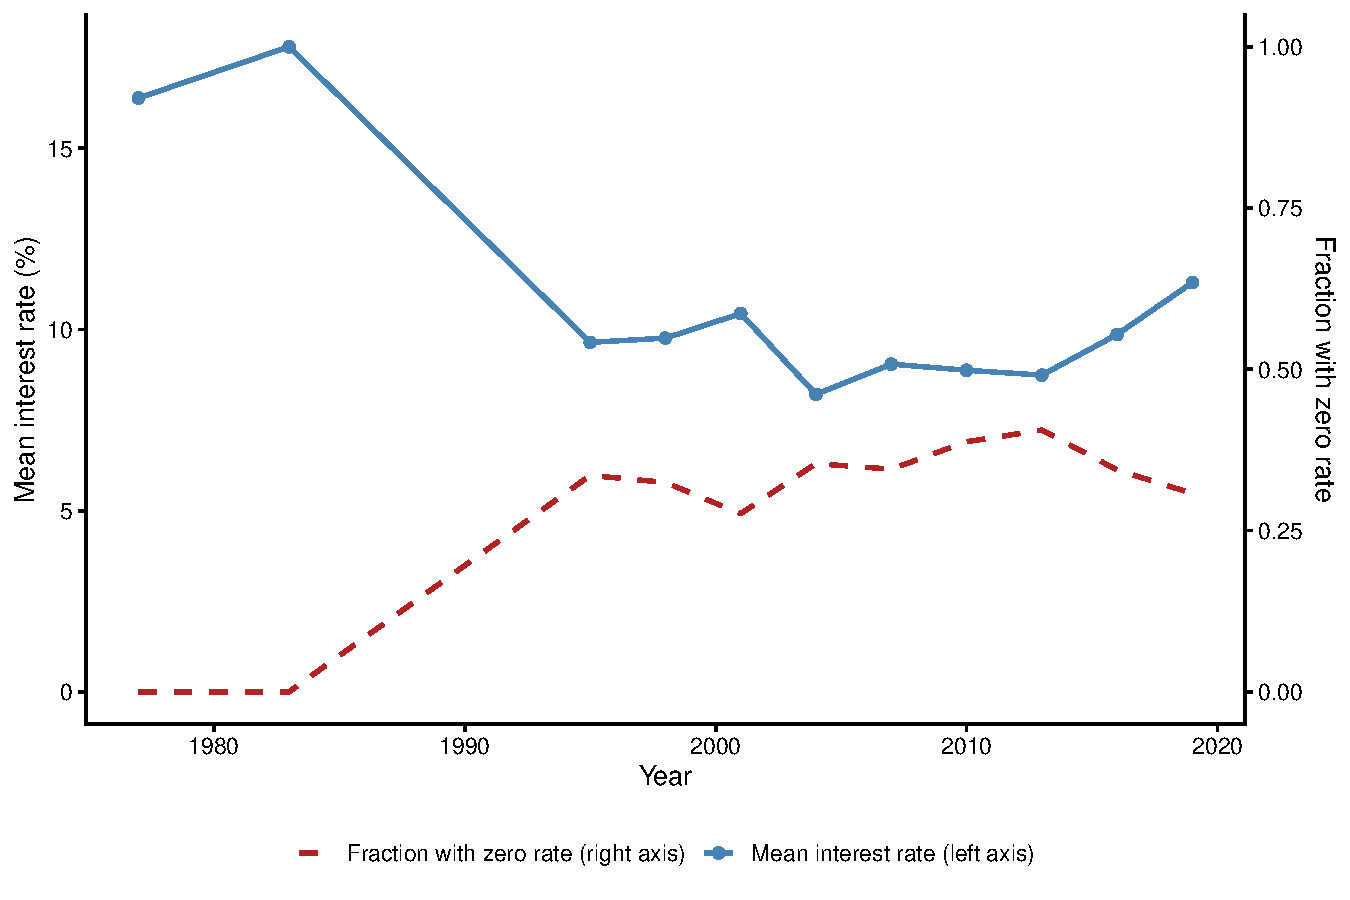
\includegraphics[width=.9\textwidth]{../Output/Figures/card_rates_raw.pdf}
  \end{center}
  \noindent \small \uline{Notes:} This figure shows the mean interest rate on credit cards over time from the Survey of Consumer Finances, with the fraction of cards carrying zero interest rates overlaid.
\end{figure}

\begin{figure}[H]
 \caption{Usury Treatment and Banking Deregulation (MSW Index)}\label{fig:msw}
 \vspace{-0.25cm}
 \begin{center}
  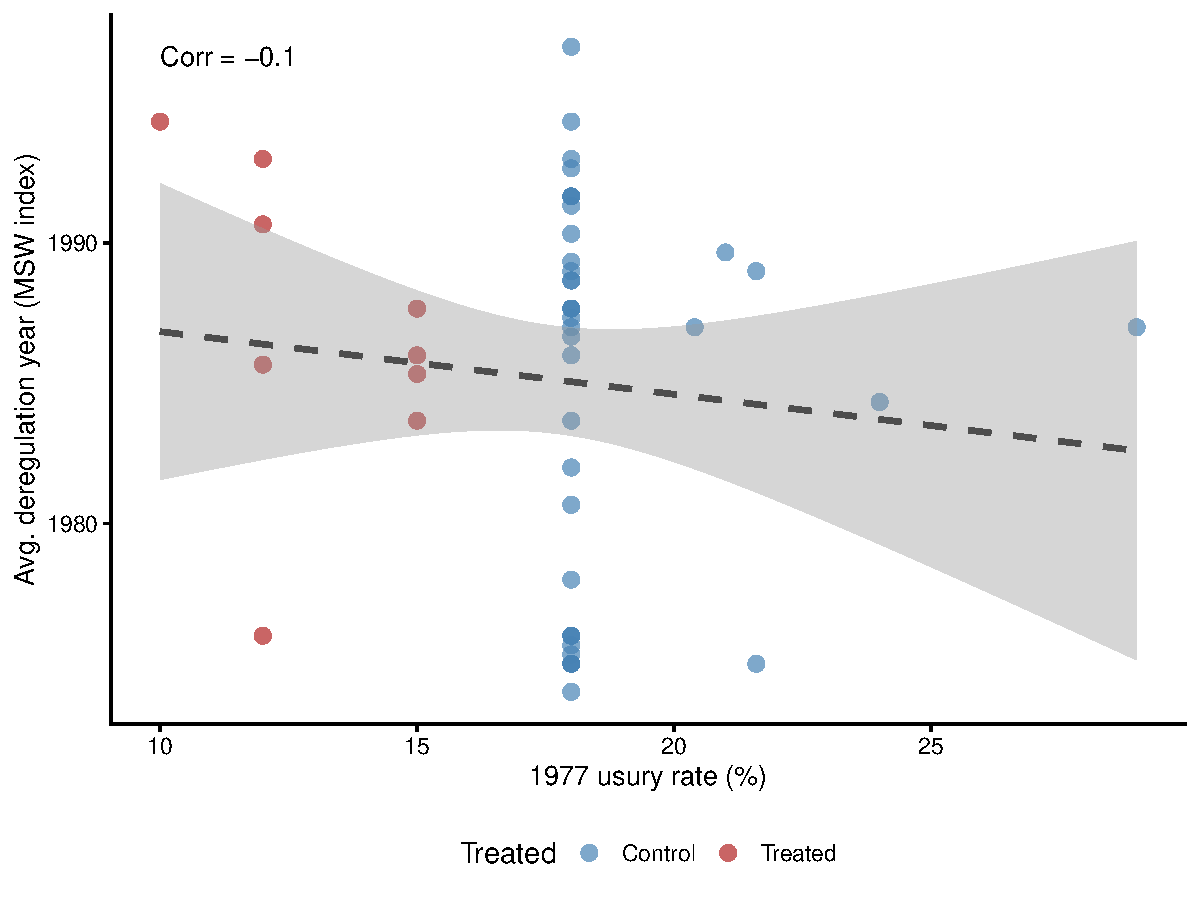
\includegraphics[width=.7\textwidth]{../Output/Figures/msw_correlation.pdf}
  \end{center}
  \noindent \small \uline{Notes:} The figure shows the correlation between states' 1977 usury rates and the average year of banking deregulation (computed from branch banking, full banking, and interstate banking deregulation dates from \cite{kroszner_regulation_2014}). The near-zero correlation supports the identifying assumption that usury treatment is orthogonal to other forms of financial deregulation.
\end{figure}

\newpage

\section{Robustness Checks}\label{sec:permutation}

A potential concern is that errors are correlated between firms selling in the same state (e.g. demand shocks at the state-level). Because firms sell in multiple states, this is not easily overcome by clustering errors at the state-of-sales level as \cite{abadie_when_2017} would typically prescribe because the outcome variable (receivables/revenue) exists at the firm level. I address by using permutation testing at the state-of-sales level (\cite{rosenbaum_design_2010}). I estimate the distribution of $\beta_{1983}$ under the null hypothesis that usury rates were randomly assigned across states in 1977 and had no effect on receivables-to-revenue ratio. To do this, I randomly sample 1,000\footnote{I would obtain Fisher-exact P-values using this procedure if I were to iterate across all 50-choose-9 = 2,505,433,700 counterfactual treatment permutations.} random possible treatment vectors, considering 1,000 alternative ways that usury rates could have been assigned in 1977. Then, I re-calculate the treatment at the firm level as described in Section 
\ref{subsec:compustat} and estimate Equation \ref{eq:dif_dif} on the counterfactual data, which is calculated on the counterfactual vector of treatments but keeping the true vector of outcomes. Figure \ref{fig:permutation} shows the results of this exercise and shows where the empirical coefficient falls in the null distribution. 

\begin{figure}[H]
 \caption{Permutation Test of $\beta_{1983}$}\label{fig:permutation}
 \vspace{-0.25cm}
 \begin{center}
  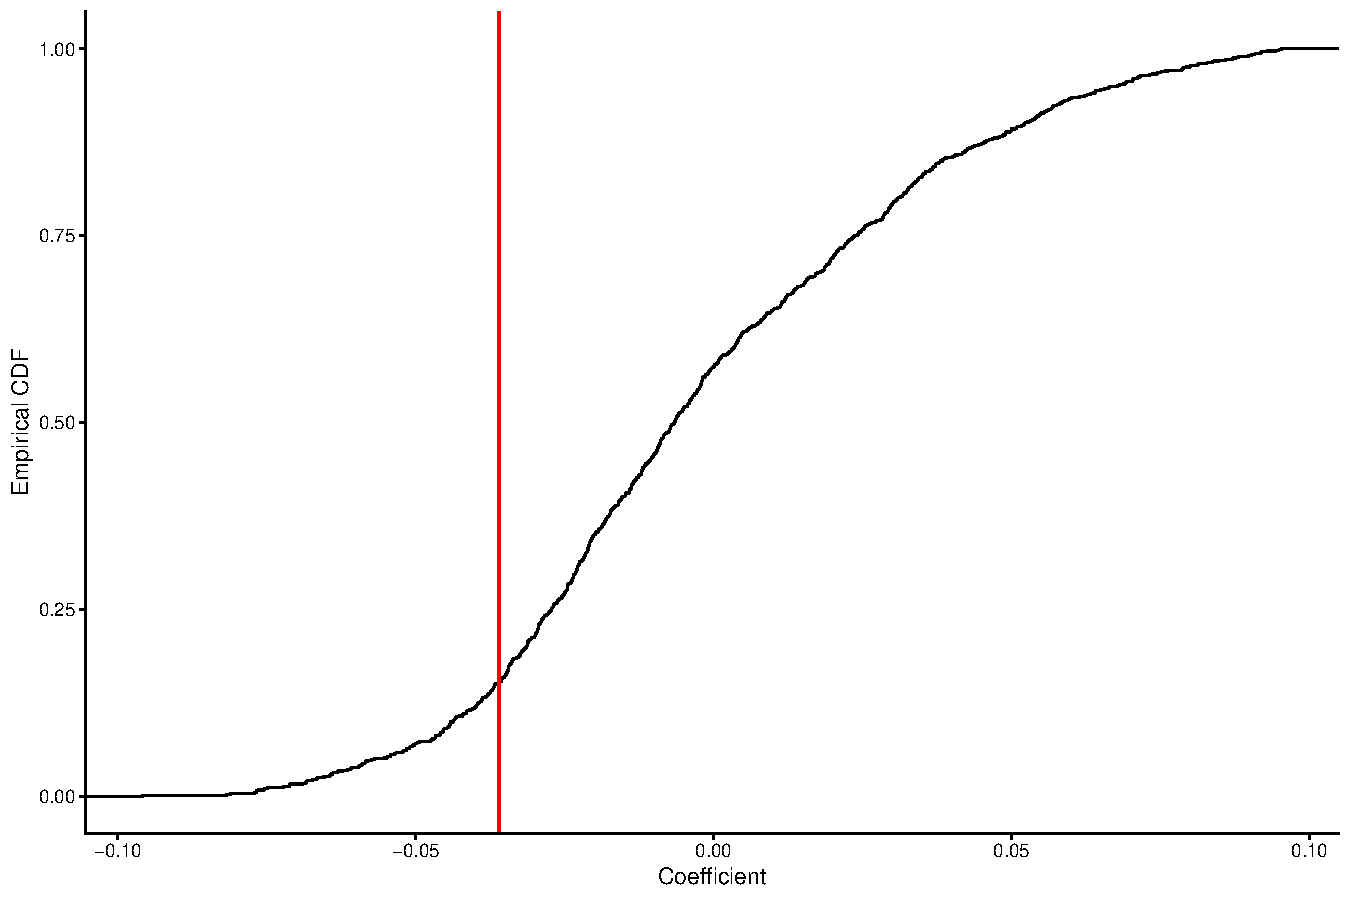
\includegraphics[width=.7\textwidth]{../Output/Figures/permutation_test.pdf}
  \end{center}
  \noindent \small \uline{Notes:} The black CDF represents the distribution of $\beta_{1983}$ under the null hypothesis that usury rates are unrelated to the receivables-to-revenue ratio. The red line represents the empirical point estimate of $\beta_{1983}$. The one-sided permutation $p$-value is 0.07.
\end{figure}
\vspace{-0.5cm}

\newpage
\section{Additional Historical Sources}\label{sec:newspapers}


\begin{figure}[!ht]
     \centering
     \begin{subfigure}[b]{0.3\textwidth}
         \centering
         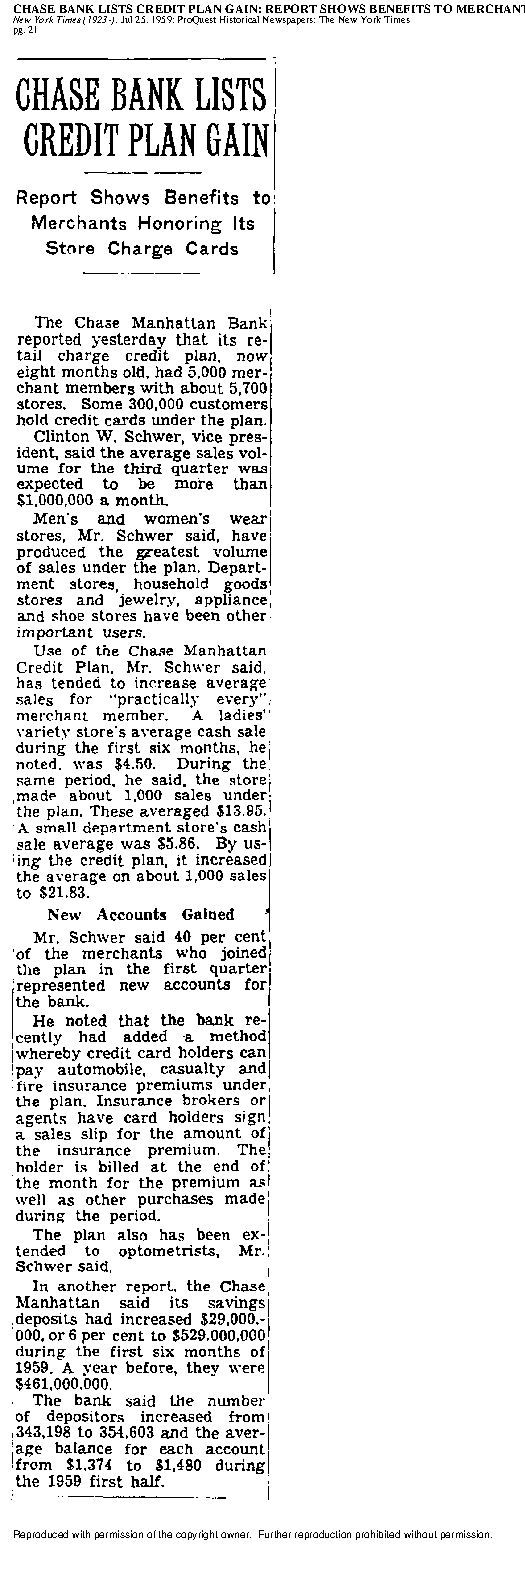
\includegraphics[width=\textwidth]{Static/CHASE_BANK_LISTS_CREDIT_PLAN_G.pdf}
     \end{subfigure}
     \hfill
     \begin{subfigure}[b]{0.5\textwidth}
         \centering
         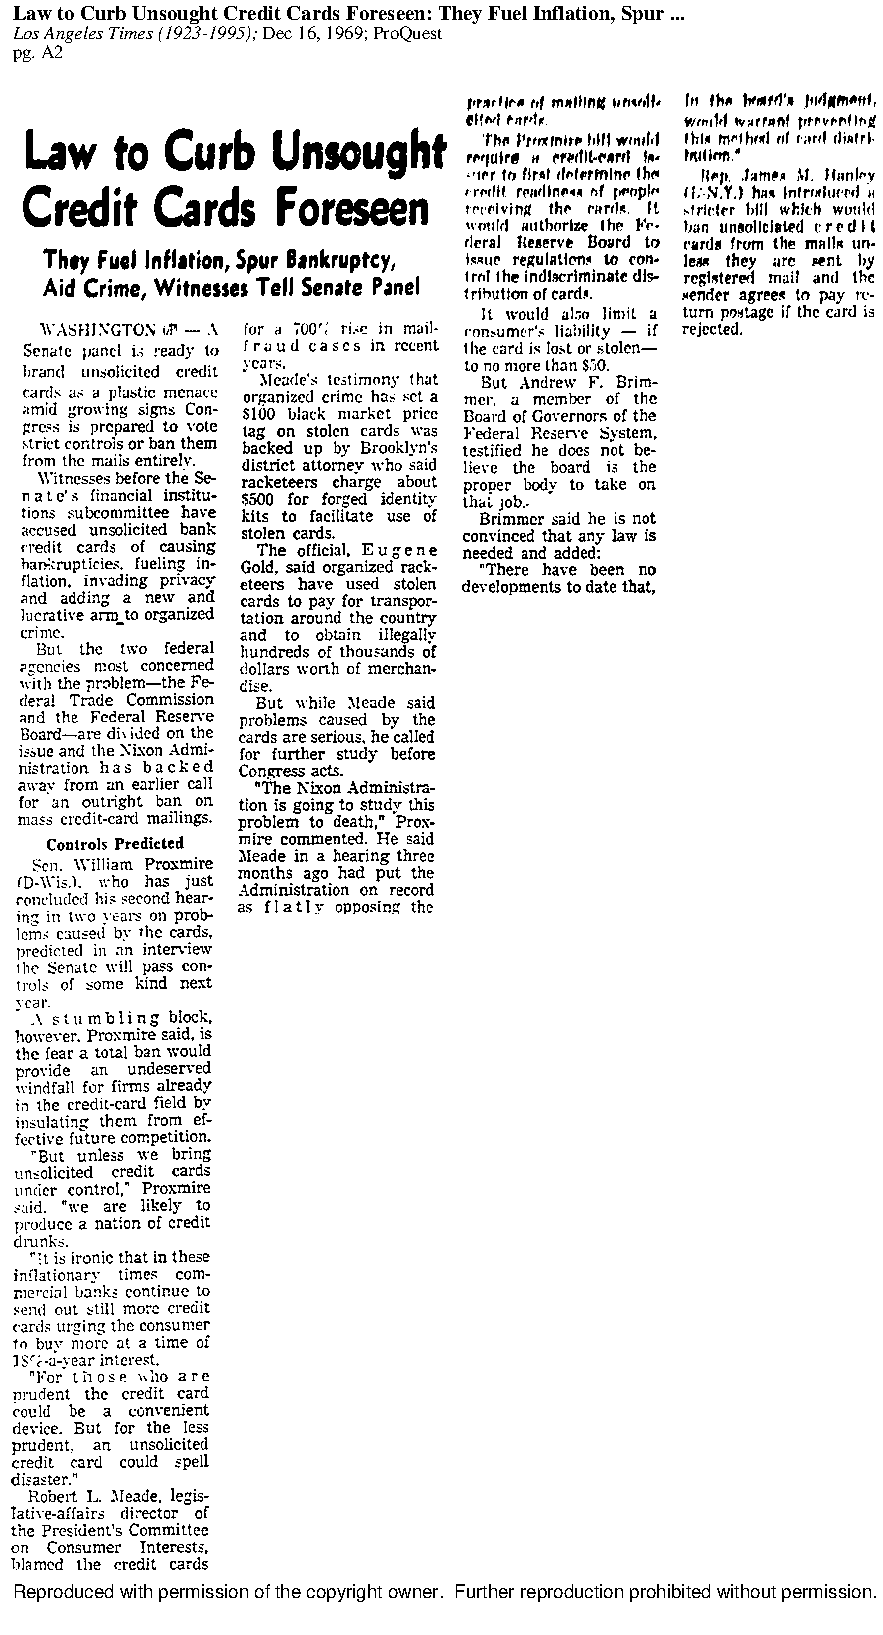
\includegraphics[width=\textwidth]{Static/Law_to_Curb_Unsought_Credit_Ca.pdf}
     \end{subfigure}
        \caption{Selected Newspaper Articles, 1959-1969}
        \label{fig:newspapers}
\end{figure}


\end{document}
